%!TEX program = xelatex
\documentclass[master,oldfontcfg,euler,twoside,openany]{cugthesis}
% 默认twoside 双面打印
% 将master修改为bachelor, doctor or master (暂时只支持硕士毕业论文模版)
% 要使用adobe字体,添加adobefonts选项
% 使用euler数学字体,如不愿使用,去掉euler
% 使用外文写作,请添加notchinese
% oldfontcfg,使用老板的字体设置,建议初学者开启

% 设置图形文件的搜索路径
\graphicspath{{pic/}}
\newcommand{\tabincell}[2]{\begin{tabular}{@{}#1@{}}#2\end{tabular}}
%仅用于本示例文档中显示特殊字符串
\usepackage{xltxtra, endnotes,hyperref, booktabs, multirow, listings, xcolor, paralist}
%仅用于子图,
%\usepackage{graphicx}
%\usepackage{subfigure}
% 文献
\renewcommand{\theendnote}{[\arabic{endnote}]}
%\setcounter{endnote}{0}
\renewcommand{\notesname}{参考文献}
%\renewcommand{\makeenmark}{\hbox{$^{[\theenmark]}$}}
\makeatletter
\def\enoteformat{
  \rightskip\z@ \leftskip\z@ \parindent=1.8em
  \leavevmode{\setbox\z@=\lastbox}\llap{\theenmark}
}
\def\enoteheading{
\noindent\chapter*{\notesname}
}
\makeatother
\renewcommand{\enotesize}{\large}

% List紧缩
\let\itemize\compactitem 
\let\enditemize\endcompactitem 
\let\enumerate\compactenum 
\let\endenumerate\endcompactenum 
\let\description\compactdesc 
\let\enddescription\endcompactdesc

%%%%%%%%%%%%%%%%%%%%%%%%%%%%%%
%% 封面部分
%%%%%%%%%%%%%%%%%%%%%%%%%%%%%%

  % 中文封面内容
  \title{基于全景漫游技术的可视化交互设计理论与实践研究}%一般情况下扉页和封皮、书脊共用一个标题文本,可以不用定义\spinetitle(仅硕博有用), \covertitle(本硕博均有用)和\encovertitle(仅本科有用)。特殊情况见下。
  \spinetitle{基于全景漫游技术的可视化交互设计理论与实践研究}
  %特殊情况1:本例中\title命令里含有换行控制字符,这会导致制作书脊的时候出现错误,例如如果你注释掉\spinetitle{...}这一行就会报错。这时需要定义一个不含换行等命令的\spinetitle,这并不表示\spinetitle里不能有任何命令——只能使用有限的命令。
  %特殊情况2:本例中标题过长,所以需要缩小书脊标题的字号。
  %特殊情况3:本例中中英文混排,由于tex竖排的原理限制,中英文基线不重合,所以需要人工调整英文的基线。具体调整量根据不同字体有所不同。
  \covertitle{基于全景漫游技术的可视化\\交互设计理论与实践研究}
  %\covertitle{中文题目第一行\\中文题目第二行}
  %不要在此调整封皮字体大小! Do not set Cover Page font size here!
  %特殊情况4:本例中\title中含有多个换行,导致标题超过了两行。根据制本厂规定,封皮标题不能超过两行。因此需要定义封皮使用的标题\covertitle. 如果你注释掉这一行,就会发现封皮不符合规定。
  \encovertitle{Research of Visual Interaction Design Theories and Applyments Based on Panorama Roaming Technology}
  %\encovertitle{English Title Line 1\\English Title Line 2\\English Title Line 3}
  %不要在此调整封皮字体大小! Do not set Cover Page font size here!
  %特殊情况5:仅本科生有用。本科封皮中有英文标题,不超过三行。与上类似。

  \author{马\ 申\ 彦}
  \depart{机械与电子信息学院}%系别,硕博请用系代号,本科请用全称如
  %\depart{数理化和信息工程系}
  \major{设计学}%专业,硕博请用全称,本科不需要
  \advisor{周晔\ 副教授}
  %\coadvisor{姚宏\ 教授}%第二导师,没有请注释掉
  \studentid{1201410655}%
  \submitdate{二〇一七年五月}
  %\numsubmitdate{2015.04}
  % 英文封面内容
  \entitle{Research of Visual Interaction Design Theories\\and Applyments Based on Panorama Roaming Technology}
  \enauthor{Shenyan Ma}
  \enmajor{Design Specialist}
  \enadvisor{Prof. Ye Zhou}
  %\encoadvisor{Prof. Hong Yao}%另外一个导师
  \ensubmitdate{2017.05}
  
%%%%%%%%%%%%%%%%%%%%%%%%%%%%%%%%%%%%%%%%%%%%%%%%%%%%%%%%%%%%%%%%%%%%%
% If you use another language instead of chinese and english, then you
% should define some strings and provide information in your language.
%%%%%%%%%%%%%%%%%%%%%%%%%%%%%%%%%%%%%%%%%%%%%%%%%%%%%%%%%%%%%%%%%%%%%
%  \otherustcstr{zhong guo ke xue ji shu da xue}%A translation of `University of Science and Technology of China' in your language
%  \otherthesisstr{shuo shi xue wei lun wen}%A translation of `A dissertation for doctor(master/bachelor)'s degree' in your language
%  \otherauthorstr{xing ming}%A translation of `Author' in your language
%  \otherdepartmentstr{yuan xi}%A translation of `Department' in your language
%  \otherstudentidstr{xue hao}%A translation of `Student ID' in your language
%  \othersupervisorstr{dao shi}%A translation of `Supervisor' in your language
%  \otherfinishedtimestr{ri qi}%A translation of `Finished Time' in your language
%  \otherspecialitystr{zhuan ye}%A translation of `Speciality' in your language
%  \othertitle{zhong guo ke xue ji shu da xue tong yong xue wen lun wen shi li wen dang}
%  \otherauthor{zhao qian sun}
%  \otheradvisor{zhou wu zheng}
%  \othercoadvisor{feng chen zhu}
%  \othersubmitdate{hou nian ma yue}
%  \othermajor{mou zhuan ye}
%  \otherdepart{mou xi}

\begin{document}

%代码
\lstset{numbers=left, 
numberstyle= \tiny, 
keywordstyle= \color{ blue!70},commentstyle=\color{red!50!green!50!blue!50}, 
frame=shadowbox, 
rulesepcolor= \color{ red!20!green!20!blue!20} 
} 

%表格换行
\renewcommand{\tabincell}[2]{\begin{tabular}{@{}#1@{}}#2\end{tabular}}

  % 封面
  \maketitle

%特别注意,以下述顺序为准,在对应部分添加文档部件,切勿颠倒顺序:
%本科论文的文档部件顺序是:
%    frontmatter:致谢、目录、中文摘要、英文摘要、
%    mainmatter: 正文章节
%    backmatter: 参考文献或资料注释、附录
%硕博论文的文档部件顺序是:
%    frontmatter:中文摘要、英文摘要、目录、符号说明
%    mainmatter: 正文章节
%    backmatter: 参考文献、附录、致谢、发表论文
%%%%%%%%%%%%%%%%%%%%%%%%%%%%%%
%% 前言部分
%%%%%%%%%%%%%%%%%%%%%%%%%%%%%%
\frontmatter
%\pagenumbering{}
\makeatletter
\ifustc@bachelor
	%%%%%%%%%%%%%%%%%
	%本科论文修改这里
	%%%%%%%%%%%%%%%%%
	% 致谢
	% !TEX root = ../main.tex
\begin{thanks}

作者研究生就读期间得到了各位老师同学的悉心帮助与指导,谢谢你们让我成为一个更好的人!

首先,感谢我的导师周晔老师,周老师从本科起就担任我们专业相关课程的授课老师,课堂上对学子淳淳教诲、言传身教,在科研上精益求精、指导我们向学术领域高峰奋进。在毕业论文开题至写作完成期间,周老师均给予了我莫大的帮助,对论文中存在的问题详细解答,使我受益匪浅。

然后,要感谢本专业其他各位老师。蔡建平老师于本科时指导我参加某全国比赛并收获佳绩,知遇之恩没齿难忘;陈晓鹂老师与我成为了科研学习方面良好的合作伙伴,一起完成了一个又一个科研实践项目;顾湘老师对我严格认真,我于研一时参与顾老师的助教工作感到十分荣幸。还有李理老师、肖畅老师、杨展老师等在我学习期间给予的帮助与支持,谢谢你们!

最后,感谢同寝室的兄弟、专业内其他同学以及我的家人,你们是我生活上最好的伙伴和后盾。

\vskip 18pt

\begin{flushright}

~~~~马申彥~~~~

\today

\end{flushright}

\end{thanks}

	
	%目录部分
	%目录
	\tableofcontents
	%默认表格、插图、算法索引名称分别为“表格索引”、“插图索引”和“算法索引”
	%如果需要自行修改lot,lof,loa的名称,请定义
	%\ustclotname{...}
	%\ustclofname{...}
	%\ustcloaname{...}

	% 表格索引
	\ustclot
	% 插图索引
	\ustclof
	%算法索引 
	%如果需要使用算法环境并列出算法索引,请加入补充宏包。
	\ustcloa
	
	% 摘要
	\begin{abstract}

全景漫游是虚拟现实技术的核心,通过模拟真实场景的全景图或视频以及不同于传统平面媒介的多通道交互手段,用户可以通过全景漫游设备或是手机屏幕等体验到身临其境般的使用体验。通过研究全景漫游相关技术,可以增强交互设计在计算机视觉及工业可视化方向上的应用价值,也帮助提升了包括旅游、通讯、建筑、资源勘探等应用领域的信息可视化程度。

本文从全景漫游发展的现状出发,列举并阐述了现有全景漫游技术的特点及需求,通过比较全景漫游多种应用的操作方式及交互流程发现其有待加强的地方。从人体生理与心理的相关特征特性出发,结合人机工程学和心理学观点深入剖析了全景漫游与人结合的难点和问题,力图以人为设计中心,加强人在全景漫游体验中的参与作用。

从图形化人机界面到信息架构再到功能模块,将全景漫游与真实世界中的游乐场场景进行类比,以交互研究的方式结合相关实例说明信息架构在人机界面的重要作用,论述了信息架构组件化和可视化的必要性。通过建立以漫游功能、导航功能、搜索功能和记忆功能为主的功能模型,列举了部分功能模块的实现要点。

在交互模型方面,以设备交互、导航交互和场景交互为切入点,以信息流的处理过程为例分析了交互操作形式的可反馈性的重要性,提出了用户在交互过程中需要进行信息修正的观点;详细阐述了信息架构的三种组织方式的应用场景,列举了自顶向下、自底向上和不可见的信息架构在模型中的具体体现:上下文感知用以建立导航间的上下文关系、增强信息用以减少用户变换注意的负担、多任务切换的合理形式以在用户记忆中留存相关信息利于语境的切换等。通过建立多层上下文语境增强语境间的联系,促进小语境间切换的适应性以及语境内部信息的流通。以场景中各种漫游路径的实现形式为基础,论述了场景中直观提供场景特殊标识存在的合理性与必要性,并给出了分层级特殊化的指示图标标识。

以实例分析的方式解释并总结了某一例全景漫游系统的交互设计及程序实现的过程,从需求分析到功能架构,以交互模型为指导原则进行可视化设计,主要从导航界面设计、漫游界面设计和功能界面设计三个方向举例交互原型设计,完成漫游系统的设计开发。同时,以 A-Frame 框架为基础,进行了简单的功能程序开发以供设计评价应用。在设计完成后,以收集用户体验数据的形式得到了用户交互操作行为的第一手资料,分析并论证了该交互设计中应用相关设计理论的可行性与成效。

本文提出了以人为中心、可视化交互为主导的全景漫游交互设计思路,从人与全景漫游的关系至全景漫游中信息架构和交互模型的分析论证中分析了全景漫游交互设计中重点功能的实现与细节的处理,为全景漫游相关设计提供了相关分析思路和实践经验。

\textbf{关键词:} 全景漫游、上下文感知、信息流、交互模型

\end{abstract}


\renewcommand{\abstractname}{Abstract}

\begin{abstract}
Panorama roaming is the basement of virtual reality technology. Users can immerse themselves in virtual environment by using panorama roaming device or mobile screen which is based on panorama image or video simulating real environment and multi-channel interaction methods excluding traditional interface media. Through reserach on panorama roaming, the implement value of interaction design in computer graphics and industrial visualization will be enhanced, as well as visualization of information in applyment fields including tourism, communication, architecture and resources exploration.

The thesis firstly lists and demonstrates characters and demands of its technology as current development of panorama roaming technology. The enhanceable details could be found by comparing serveral operative methods and interaction flow of ranorama roaming. The difficulties and problems between panorama roaming and human beings are explained according to ergonomics and psycology, with study on related human physical and psycologic characters. Interaction design will treate human as the middle part of roaming and enhance participation of human in roaming experience.

Methods of interaction researches connected to related applyment practice which are taken in flow of graphic interface, information architecture and functional module, comparison between panorama roaming and amusement park in orderto demonstrate fundemental function 
of information architecture in human-computer interface and its necessity of modularism and visualization of information architecture. The applyment details of specific functional modules are listed through making functional model based on roaming function, navigation function, search function and memory function.

In the part of interaction model, the importance of feedback in interactive operations is analyzed for examplex of information flow process at the point of device interaction, navigation interaction and environment interaction. The view point of user information revision is raised in interaction progress. The applyment fields of three types of interactive operation organization, as known as top-to-bottom, bottom-to-top and invisible forms, are demonstrated with their detailed implement: Context perception carries out context relationship between navigation layers, which enhances information to avoid rapid switching concern of user and keep memories in mind to benefit switch of context by making multi-task switch more reasonable. Multi-layer context is set up to enhance relationship between contexts which benefits both adaption of switch in minor context and context inner information transition. The reasonablity and necessity of existence of direct scene specific mark are demonstrated on base of implement of roaming routes, and layer-specialed guide icon marks are raised for example.

One case of panorama roaming system is detailed and concluded by practice analysis in interaction design and program implement. The work flows from requirement analysis to function architecture, visually developped in guide of interaction model. Interaction prototype design takes examples of navigation interface, roaming interface and function interface design contributing to development of roaming system. A-Frame which known as a web Javascript framework is applied in functional programme development with its extra components to meet the evaluation of design. User experience data is collected immediately after user interaction operation as the original profile which is used for analyzing feasibility and efficiency of related theories in interaction design.


The thesis raised one kind of human-oriented panorama roaming interaction design strategy leading by visualization interaction. Analysis on relationship between human and roaming, demostration of information architecture and interaction model draws the picture of panorama roaming interaction design function implement and detailed process. All above could be fundamental analysis strategy and practical experience for related designs.

\textbf{Keywords: } panorama roaming, context perception, information flow, interaction model

\end{abstract}




%此文件中含有中英文摘要
\else
	%%%%%%%%%%%%%%%%%
	%硕博论文修改这里
	%%%%%%%%%%%%%%%%%
  % 个人简介
  % !TEX root = ../main.tex
\chapter*{作者简介}
 %\thispagestyle{empty}
\begin{spacing}{1.3}

马申彥,男,江苏无锡人,1992 年 4 月出生,
中国地质大学(武汉)机械与电子信息学院在读研究生。本科于中国地质大学(武汉)机械与电子信息学院就读工业设计系。硕士研究生在读期间,致力于产品数字化设计与 Web 技术的研究,曾参与若干校级科研项目,并进行了多次社会实践活动,在产品设计的可视化、设计成果多媒体展示和网页交互设计与程序实现等领域有所研究。

% \input{chapter/pub}
\end{spacing}

\subsection*{参与的科研项目}
\begin{description}
	\item[面向产品设计的 VDP 人机功效模块实验技术研究] 实验数据整理与分析
	\item[基于VDP虚拟仿真软件的机电产品三维可视化设计研究] 学校开放实验室项目,负责人
\end{description}

\vskip 12pt

\subsection*{发表的专利}
\begin{description}
	\item[羽毛球发球器](专利号:ZL.2016305833384)
	\item[折叠式台灯](专利号:ZL.2016305833613)
\end{description}

\vskip 12pt

\subsection*{参与的社会实践}
\begin{description}
	\item[2015.7 - 2015.11] 广东顺德工业设计研究院(设计类实习生)
	\item[2016.3 - 2016.7] 苏州蜗牛数字科技有限公司(前端开发工程师实习)
	\item[2016.10 - 2017.1] 豆瓣阅读(前端开发工程师实习)
\end{description}
  % 摘要
  % !TEX root = ../main.tex
\begin{cnabstract}
\begin{spacing}{1.0}
%\thispagestyle{empty}
全景漫游是虚拟现实技术的核心,通过模拟真实场景的全景图或视频以及不同于传统平面媒介的多通道交互手段,用户可以通过全景漫游设备或是手机屏幕等体验到身临其境般的使用体验。通过研究全景漫游相关技术,可以增强交互设计在计算机视觉及工业可视化方向上的应用价值,也帮助提升了包括旅游、通讯、建筑、资源勘探等应用领域的信息可视化程度。

本文从全景漫游发展的现状出发,列举并阐述了现有全景漫游技术的特点及需求,通过比较全景漫游多种应用的操作方式及交互流程发现其有待加强的地方。从人体生理与心理的相关特征特性出发,结合人机工程学和心理学观点深入剖析了全景漫游与人结合的难点和问题,力图以人为设计中心,加强人在全景漫游体验中的参与作用。

从图形化人机界面到信息架构再到功能模块,将全景漫游与真实世界中的游乐场场景进行类比,以交互研究的方式结合相关实例说明信息架构在人机界面的重要作用,论述了信息架构组件化和可视化的必要性。通过建立以漫游功能、导航功能、搜索功能和记忆功能为主的功能模型,列举了部分功能模块的实现要点。

在交互模型方面,以设备交互、导航交互和场景交互为切入点,以信息流的处理过程为例分析了交互操作形式的可反馈性的重要性,提出了用户在交互过程中需要进行信息修正的观点;详细阐述了信息架构的三种组织方式的应用场景,列举了自顶向下、自底向上和不可见的信息架构在模型中的具体体现:上下文感知用以建立导航间的上下文关系、增强信息用以减少用户变换注意的负担、多任务切换的合理形式以在用户记忆中留存相关信息利于语境的切换等。通过建立多层上下文语境增强语境间的联系,促进小语境间切换的适应性以及语境内部信息的流通。以场景中各种漫游路径的实现形式为基础,论述了场景中直观提供场景特殊标识存在的合理性与必要性,并给出了分层级特殊化的指示图标标识。

以实例分析的方式解释并总结了某一例全景漫游系统的交互设计及程序实现的过程,从需求分析到功能架构,以交互模型为指导原则进行可视化设计,主要从导航界面设计、漫游界面设计和功能界面设计三个方向举例交互原型设计,完成漫游系统的设计开发。同时,以 A-Frame 框架为基础,进行了简单的功能程序开发以供设计评价应用。在设计完成后,以收集用户体验数据的形式得到了用户交互操作行为的第一手资料,分析并论证了该交互设计中应用相关设计理论的可行性与成效。

本文提出了以人为中心、可视化交互为主导的全景漫游交互设计思路,从人与全景漫游的关系至全景漫游中信息架构和交互模型的分析论证中分析了全景漫游交互设计中重点功能的实现与细节的处理,为全景漫游相关设计提供了相关分析思路和实践经验。

\keywords{全景漫游、上下文感知、信息流、交互模型}
\end{spacing}
\end{cnabstract}


\begin{enabstract}
\begin{spacing}{1.0}
%\thispagestyle{empty}
Panorama roaming is the basement of virtual reality technology. Users can immerse themselves in virtual environment by using panorama roaming device or mobile screen which is based on panorama image or video simulating real environment and multi-channel interaction methods excluding traditional interface media. Through reserach on panorama roaming, the implement value of interaction design in computer graphics and industrial visualization will be enhanced, as well as visualization of information in applyment fields including tourism, communication, architecture and resources exploration.

The thesis firstly lists and demonstrates characters and demands of its technology as current development of panorama roaming technology. The enhanceable details could be found by comparing serveral operative methods and interaction flow of ranorama roaming. The difficulties and problems between panorama roaming and human beings are explained according to ergonomics and psycology, with study on related human physical and psycologic characters. Interaction design will treate human as the middle part of roaming and enhance participation of human in roaming experience.

Methods of interaction researches connected to related applyment practice which are taken in flow of graphic interface, information architecture and functional module, comparison between panorama roaming and amusement park in orderto demonstrate fundemental function 
of information architecture in human-computer interface and its necessity of modularism and visualization of information architecture. The applyment details of specific functional modules are listed through making functional model based on roaming function, navigation function, search function and memory function.

In the part of interaction model, the importance of feedback in interactive operations is analyzed for examplex of information stream process at the point of device interaction, navigation interaction and environment interaction. The view point of user information revision is raised in interaction progress. The applyment fields of three types of interactive operation organization, as known as top-to-bottom, bottom-to-top and invisible forms, are demonstrated with their detailed implement: Context perception carries out context relationship between navigation layers, which enhances information to avoid rapid switching concern of user and keep memories in mind to benefit switch of context by making multi-task switch more reasonable. Multi-layer context is set up to enhance relationship between contexts which benefits both adaption of switch in minor context and context inner information transition. The reasonablity and necessity of existence of direct scene specific mark are demonstrated on base of implement of roaming routes, and layer-specialed guide icon marks are raised for example.

One case of panorama roaming system is detailed and concluded by practice analysis in interaction design and program implement. The work flows from requirement analysis to function architecture, visually developped in guide of interaction model. Interaction prototype design takes examples of navigation interface, roaming interface and function interface design contributing to development of roaming system. A-Frame which known as a web Javascript framework is applied in functional programme development with its extra components to meet the evaluation of design. User experience data is collected immediately after user interaction operation as the original profile which is used for analyzing feasibility and efficiency of related theories in interaction design.


The thesis raised one kind of human-oriented panorama roaming interaction design strategy leading by visualization interaction. Analysis on relationship between human and roaming, demostration of information architecture and interaction model draws the picture of panorama roaming interaction design function implement and detailed process. All above could be fundamental analysis strategy and practical experience for related designs.

\enkeywords{panorama roaming, context perception, information stream, interaction model}
\end{spacing}
\end{enabstract}
%此文件中含有中英文摘要
	% 目录
	\tableofcontents
	%默认表格、插图、算法索引名称分别为“表格索引”、“插图索引”和“算法索引”
	%如果需要自行修改lot,lof,loa的名称,请定义
	%\ustclotname{...}
	%\ustclofname{...}
	%\ustcloaname{...}

	% 表格索引
	%\ustclot
	% 插图索引
	%\ustclof
	%算法索引 
	%如果需要使用算法环境并列出算法索引,请加入补充宏包。
	%\ustcloa
	
	%符号说明,需要加入补充包
	%\include{chapter/denotation}%不是必需的,如果不想列出请注释掉
\fi
\makeatother

%%%%%%%%%%%%%%%%%%%%%%%%%%%%%%
%% 正文部分
%%%%%%%%%%%%%%%%%%%%%%%%%%%%%%
\mainmatter

  \xiaosi
  % \include{chapter/chap-intro}
  % \include{chapter/chap-analytics}
  % \include{chapter/chap-IntermediateAnalysis}
  % \include{chapter/chap-memomr}
  % \include{chapter/chap-experiment}
  %\include{chapter/chap-application}
  % \include{chapter/chap-summary}
  %自行添加
  %\include{chapter/...}
  % \chapter{全景漫游技术与设计}
\section{全景漫游的目的}
古语云:眼观六路,耳听八方

这句话本意是形容人机制灵活,遇事能多方观察分析。而如今科技进步迅猛、社会发展气象万千,古时人们所向往的“千里眼”和“顺风耳”早已成为了现实(卫星雷达和手机电话),信息获取效率相比于古代有了巨大的提升。人们真正地做到了“眼观六路,耳听八方”。但这些技术往往只是片面地延展了人的感官能力,只是将人与物间某些距离拉近了,少有将人作为感官系统的中心来进行考量。在现代信息通讯过程中,人被排除在计算机的屏幕之外,人和真正的信息之间有一层薄薄的但难以直接触碰的玻璃阻隔。

古希腊的哲学家普罗泰戈拉说过:“人是万物的尺度,是存在的事物存在的尺度,也是不存在的事物不存在的尺度。“。借助现有科学技术,可以轻易地观摩到深入海底数公里的珊瑚礁分布、险象环生的热带雨林内生物的栖息环境、甚至是浩瀚无垠的太空中星象奇观。面对如此美景,只是观赏单一的图像帧序列来企图感受自然的奥妙总是觉得少了一份身临其境的体验。

人并不是一定要盯着一块显示屏。显然可得的想法就是利用显示屏将人的视线包裹起来,这样观察起来具有良好的主动性和体验感,同时规避了将人置于一些特殊环境所带来的附加成本或是风险因素。虽是虚拟,胜似现实,这就是“虚拟现实”的意义。而“全景漫游”则是“虚拟现实”中最重要的一部分。

\section{全景漫游的现状}
全景漫游是当今互联网行业发展最为迅速的技术之一,它是虚拟现实(即 VR 技术)的基础。沉浸性和交互性是其得到众多用户青睐的最主要原因,可供用户身临其境般体验的图形化界面,以及不同于传统平面媒介的交互手段共同促进了全景漫游技术的推广。
全景漫游解决了传统工业界对于空间概念呈现形式不足的痛点,通过定义场景的 360 度无缝全景图像,仿佛使人置身于制作者脑海中设计出的环境内,配合移动设备内置陀螺仪支持的重力感应功能,足不出户即可感受任何可以用图像表达的场景。80 天环游地球不再只是一个梦想,而且现今全景播放设备层出不穷,最便宜的 Google Cardboard 制作成本不足一元钱,人人 VR 的时代即将到来。

\section{全景漫游与设计结合的必要性}
设计行业向来紧跟时代发展潮流,全景漫游技术已经发展地比较成熟,因其本身具有互联网基因,故将其移植至设计产业的成本相较传统的工业技术会显著降低。传统产品原型技术将产品制作模型交付演示的时代可能即将被虚拟化技术所取代,相伴随的是设计成本的减轻以及设计迭代的加速。
将全景漫游技术引入设计行业的难点在于将全景展示的程式化模型转化为用户可探索、可理解、可学习的交互模型,现阶段的问题在于用户进入场景之后因场景与以往二维界面的割裂而导致心理产生的不适应性使其手足无措。值得研究的重点环节是降低用户的初次体验成本,加深用户记忆中对操作流程感悟的交互模型,最终达到用户无缝体验设计师所要传达的设计意图的目的。

\section{全景漫游中可视化交互理论研究的意义}
本课题旨在探索全景漫游场景中应用程序接口与用户心智模型的转化过程,通过分析场景程序执行的逻辑,用户操作的普适性规律以及人类学习行为的通常过程,将三者有机结合,以场景插件程序的形式进行封装,并提取出相应的 API 接口,以供本课题其后实例开发及其他对本课题感兴趣的开发者使用。
可视化技术对于工业发展的提升是显然的,从传统的制图学到近代的计算机辅助制图,再到现今的三维模拟技术,工业界向来拥抱可视化技术的前沿。可视化交互的意义就在于将图形化表述的产品按照其功能有机地组合起来,以可体验的形式呈现给用户/开发者。不再需要对产品的每部分组成有基础的了解也可认知其完成状态,也就意味着机械产品设计的成本进一步降低,普及到每个想要创造的人身上进而使其创造出更多产品的可能性变得现实。\ref{fig:test}

\begin{figure}[htp]
\centering

\includegraphics[width=.5\textwidth]{profile}
\label{fig:test}
\caption{test}
\end{figure}
  \chapter{绪论}

交互设计是一种设计并定义人造系统内多个个体间交流的内容与结构,使之互相配合,以达成某种目的的行为。交互设计早在 20 世纪 80 年代就作为一门新兴学科诞生了,但随着计算机及互联网行业的飞速发展,软件界面相比传统硬件界面交互信息层级更为复杂,交互方式更为多样化,交互设计才从网页设计和图形设计中独立开来,成为一个专门的领域。让用户更为高效、准确地进行交互操作,完成使用目的,并得到交互过程中的愉悦感,这是交互设计的根本目的。交互设计当前主要的设计领域包括网页、移动端操作系统和应用、电脑操作系统和应用和其他终端系统及应用等。

全景漫游是当今互联网行业发展最为迅速的技术之一,它是虚拟现实(即 VR 技术)的基础。沉浸性和交互性是其得到众多用户青睐的最主要原因,可供用户身临其境般体验的图形化界面,以及不同于传统平面媒介的交互手段共同促进了全景漫游技术的推广。

全景漫游解决了传统工业界对于空间概念呈现形式不足的痛点,通过定义场景的 360 度无缝全景图像,仿佛使人置身于真实环境内,配合移动设备内置陀螺仪支持的重力感应功能,足不出户即可感受任何可以用图像表达的场景。80 天环游地球不再只是一个梦想,而且现今全景播放设备层出不穷,最便宜的 Google Cardboard 制作成本不足一元钱,人人 VR 的时代即将到来。

\section{研究背景}
当前交互设计的研究重点大多数着眼于基于平面屏幕设备的交互过程,比如手机屏幕上的交互等。屏幕交互的特点是:显示屏幕形态为矩形较为规则,人与屏幕的距离较远,屏幕的可视区域不会随着视线的改变而改变等。而全景漫游所支持的设备屏幕为两个凸透镜状镜片,用户所观察到的“屏幕”边界不明显,可以通过转动头部进行改变视角视野的观察,这与一般的交互设计的设计主体有了明显的不同。并且全景漫游中信息层级被刻意弱化了,但强调了场景的完整性,这一点与传统的以页面层级对用户信息界面进行划分的交互形式也有所区别。如何利用全景漫游合理地布置交互元素,并构建合理的交互形式以期符合用户的认知模型,从而让用户在使用全景漫游时能够高效愉悦地进行体验,是全景漫游中交互设计所研究的重点。

\begin{figure}[htp]
\centering
\fbox{
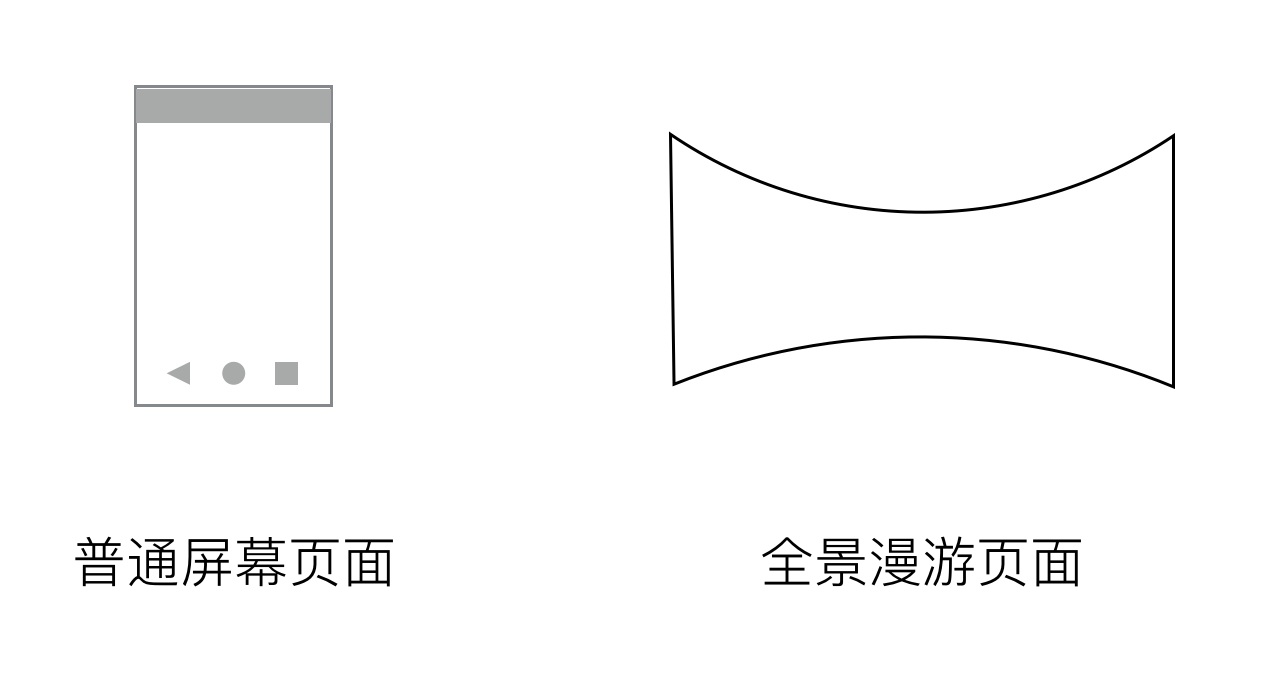
\includegraphics[width=.5\textwidth]{screen}
}
\caption{普通屏幕页面与全景漫游界面}
\label{fig:screen}
\end{figure}

交互设计领域当前已有相当多的研究成果,例如人机交互界面(即 HCI)相关学科和理论一直是国际上计算机相关学科研究的重点,辛向阳教授将人与系统交互的过程分解为了五个要素,分别为:用户、行为、目标、场景、媒介(peopl、actions、means、purpose、contexts)。拥有良好的科研氛围和市场实践经验,交互设计的学科体系已然较为成熟。再看到全景漫游这一方面,其计算机相关理论也较为成熟,相关的图像信号捕捉处理算法已被大范围应用与实践中,各种根据特殊用途产生的适配处理也增强了全景漫游相关应用的鲁棒性。例如,在敦煌石窟数字化工作中的洞窟全景漫游技术初步应用一文\endnote{宋利良,李大丁. 敦煌石窟数字化工作中的洞窟全景漫游技术初步应用[J]. 敦煌研究,2010,(06):93-97.}中,作者以高动态范围影像( HDR)处理为例说明了敦煌石窟数字化工作在拍摄全景图像至后期处理中遇到的难点和问题。

与技术成熟相对的是,全景漫游方面的交互研究一直停留在起步阶段。在中国知网(cnki.net)上搜索“全景漫游 设计”,命中 359 条结果,搜索“全景漫游 技术“,命中 712 条结果。其中,“全景漫游 设计”的命中结果中有大部分为“程序设计”的相关论文,故可以得出国内相关设计研究尚未达到成熟,全景漫游相关设计理论仍有较大的发展空间。如何将全景漫游的技术应用到交互设计中,将两者有机结合,扩展交互设计的应用领域。

\section{研究目的}
本研究试图扩展交互设计的应用领域,将全景漫游中原本简单易见的场景架构扩充为复杂的漫游系统架构,适宜用户利用全景漫游进行包括但不限于场景漫游行为的操作。从交互角度解释全景漫游中各组件的作用,利用交互设计中的信息架构模型和交互模型等思想,分析全景漫游中相应模型与传统界面的区别之处,并结合人机工程学的观点对人在漫游中的作用进行探究。研究将以理论结合实践,借鉴实际应用中已经成熟的交互方案,从用户为中心的角度出发进行整体架构及布局,并通过实际项目设计进行案例分析深入探讨理论应用于实践的形式。

\section{研究内容}
本文采用以文献阅读法为基础,采用规范研究法为主要研究方法,通过已知现象和经验为基础,以理论推导相关实践形式的价值判断,并据此完成相关设计工作,最后以定量分析和定性分析结合的形式对全景漫游中可视化交互理论成果进行检验。

研究范围为全景漫游与人的关系(从人机工程学和认知心理学角度进行分析)、全景漫游的多通道交互形式、全景漫游的信息架构、功能模型与交互模型、全景漫游可视化交互的评价体系。

本文研究步骤如下

\begin{description}
\item[第一部分] 通过文献阅读、资料检索及市场调查的方式对市面上已有的全景漫游产品及技术进行整理分析,概括全景漫游发展趋势及现状。

\item[第二部分] 从人出发,通过结合人机工程学及认知心理学的观点,对人进行全景漫游中所遇到的与一般界面交互不同的行为进行比较,并探究全景漫游中技术上具有可行性、并且与人的常规认知所匹配的交互形式。

\item[第三部分] 以界面所共有的信息架构为研究对象,从信息组织形式角度出发,阐述交互设计在全景漫游中所需要解决的实际问题。针对全景漫游设计其特有的交互形式,提取出交互模型以作设计参考。

\item[第四部分] 将以前文所梳理的全景漫游中可视化设计的理论知识为基础,以项目为设计对象通过需求定义、功能分析、设计模型、原型设计的方式进行设计实践。

\item[第五部分] 通过定量分析和定性分析的双重方法建立全景漫游中可视化交互设计的设计评价标准,并对前文中设计实例进行试评价。

\end{description}

\section{研究意义}
交互设计起源之初仅仅考虑使用键盘和鼠标进行交互操作的形式,直至进入移动时代,人们习惯于使用手指直接触摸屏幕操作,交互的内容和形式均得到了扩充。与用户所见到的交互界面不同,设计师在进行设计时所建立的信息架构与交互模型在屏幕界面上是隐形的,故交互设计的意义在于通过隐式的模型建立出实际可行的显式的交互形式。

研究全景漫游的可视化交互的意义在于:
\begin{enumerate}
	\item 将交互设计引入全景漫游的体验中,有助于建立科学有效的交互模型,从架构层面改善优化全景漫游的应用体验,增强用户的使用满意度
	\item 全景漫游的发展长期依赖于技术的进步,而忽视了设计在其中所占的重要作用。建立基于全景漫游技术的可视化交互理论,能够将技术与设计有机地结合起来,互取所长。
	\item 将全景漫游相关设计理论补充入交互设计中形成反哺,可以拓展交互设计的应用领域,利用实践增强其可信性。
\end{enumerate}


  \chapter{全景漫游行业的市场现状}

\section{全景漫游技术总览}

全景漫游技术按载体分类可分为:
\begin{enumerate}
\item{\emph{场景捕获硬件技术:}视频捕获设备及其保障设备,用以采集全景漫游的视频、图片、音频等素材。}
\item{\emph{场景呈现硬件技术:}主要包括 VR 眼镜、VR 互动手柄、VR 主机等。}
\item{\emph{场景处理技术:}场景规划设计、场景素材的保存与传输以及相应程序开发等。}
\item{\emph{场景还原与增强技术:}将场景素材与功能模块有机地整合,提供给用户身临其境般的全景漫游体验。}
\end{enumerate}

\subsection{场景呈现硬件技术}
相对而言,硬件技术相比于后两者进入门槛更高。目前市场上三大 VR 硬件厂商 OculusRift、HTCVive 和 PlayStationVR 几乎垄断了高端 VR 播放设备市场。之后加入 VR 市场的企业(如暴风、大朋、3Glasses、蚁视等)几乎都放低了姿态,推出了价格低廉但基本满足播放功能的入门级 VR 眼镜作为卖点。但随着 Google Cardboard 的推出,这款几乎没有成本可言的开源“硬件”迅速占领了低端 VR 硬件行业相当客观的市场份额。

\subsection{场景捕获硬件技术}
场景捕获技术的难点在于实时捕获,合成全景照片是一般手机都拥有的功能,大致原理就是捕获数张连续且相近的照片并通过算法进行合成球形场景。但实时场景捕获硬件的成本因其同步的特性更为高昂,目前市面上已有的厂商例如 Google JUMP、NOKIA OZO 等均是将现有平面镜头进行堆叠排布并通过后期处理合成虚拟场景,且这种方式因需要较多的镜头来堆砌同时刻的画面所以硬件成本非常高。目前市面上尚只有堆叠摄像头这一种方式进行全景场景捕获,而光场摄影等技术仍处在技术攻关阶段,相信不远的将来有可能出现消费级的场景捕获硬件。

\subsection{场景处理技术}
场景处理是目前全景漫游软件领域需要重点攻克的最大难关,但市面上各企业已基本做到自给自足的技术支持。全景漫游所依赖的基础是图像信号的捕获、加工与储存,而这些方面已有较多成功经验。目前 Web 端视频播放协议有以下两种:Real Time Messaging Protocol(实时消息传输协议,简称 RTMP)和 HTTP Live Streaming(HTTP 渐进下载,简称 HLS)。这两者是孑然不同的两种协议,而且 iPhone 等手机由于不自带支持 Flash 播放,一般考虑全端支持的流媒体播放会选用 HLS 作为传输协议,即对视频做切片,边播放边加载下一时段的切片。

\subsection{场景还原与增强技术}
场景还原与增强是与用户直接相连的部分,可以说前面的技术都是起为其保驾护航的功能。其中场景还原部分为计算机图形学的范畴,例如图像在空间上的曲率计算等,主要涉及到的技术有 OpenGL/WebGL 等,用于将二维图像还原成球状的场景。而场景增强技术则是本文所讨论的重点,其又分前处理和后处理两种,但因场景搭建的过程比较复杂,所以两种处理模式界限并不是特别清晰。

\paragraph{场景前处理代表:Unity3D}

Unity3D 是由 Unity Technologies 开发的一个让玩家轻松创建诸如三维视频游戏、建筑可视化、实时三维动画等类型互动内容的多平台的综合型游戏开发工具,是一个全面整合的专业游戏引擎。\endnote{http://t.cn/RJDzA1F}

\paragraph{场景后处理代表:Krpano}
Krpano 是一个小巧灵活的用来呈现各种全景图像和交互式的虚拟之旅的高性能全景查看器。可作为 Flash 和 HTML5 应用程序在 Web 上使用。并附有利用拖拽全景生成场景的 Krpano Tools 以供开发者快速生成用以展示的全景场景。本文将应用其进行部分设计案例的制作与演示。

\paragraph{场景后处理代表:Aframe}
Aframe 是一个用 Web 技术构建 VR 体验的框架。使用 HTML 语言及实体组件来构建场景,可应用于 web/mobile 和其他多种设备端。本文将应用其进行部分设计案例的制作与演示。

\section{全景漫游市场前景}

2016 年,随着三大 VR 设备开始出售,未来 2-3 年 VR 设备普及率将快速提升。到达 2020 年,虚拟现实生态圈将初步形成,内容、服务等盈利模式逐步成熟,全球 VR 市场规模将达到 404 亿美元,VR 游戏市场规模将达到 149.5 亿美元。\endnote{http://vreyes.baijia.baidu.com/article/595977}

虚拟现实(VR/AR)产业市场具有良好前景,2015 年中 国虚拟现实行业市场规模为 15.4 亿元人民币。融资方面,国内 VR/AR 领域投资活跃度从 2015 年开始显著提升,2015 年第四季度和 2016 年第一季度的融资额均接近 10 亿元。其中显示设备融资占据首要地位,2015 年融资案例数量占比 30\%,融资额占比 69\%;内容制作的融资案例数量虽然占比 22\%,但融资额仅占比 6\%\endnote{http://www.elecfans.com/vr/444138.html}。可见 VR 及全景漫游方向的内容制作生产领域仍处于起步阶段,与硬件厂商等差距较大,但同时其中也孕育了巨大的商机。

VR 内容开发受市场认可,线下体验馆增长迅速。由于中国 VR 市场主流设备仍以移动端 VR 眼镜为主,VR 视频内容的开发数量要远多于 VR 游戏内容。VR 平台上已有约 2700 款视频和 800 款游戏。预计 2020 年中国 VR 设备出货量 820 万台,用户量超过 2500 万人,见图\ref{fig:market}。

\begin{figure}[htp]
\centering
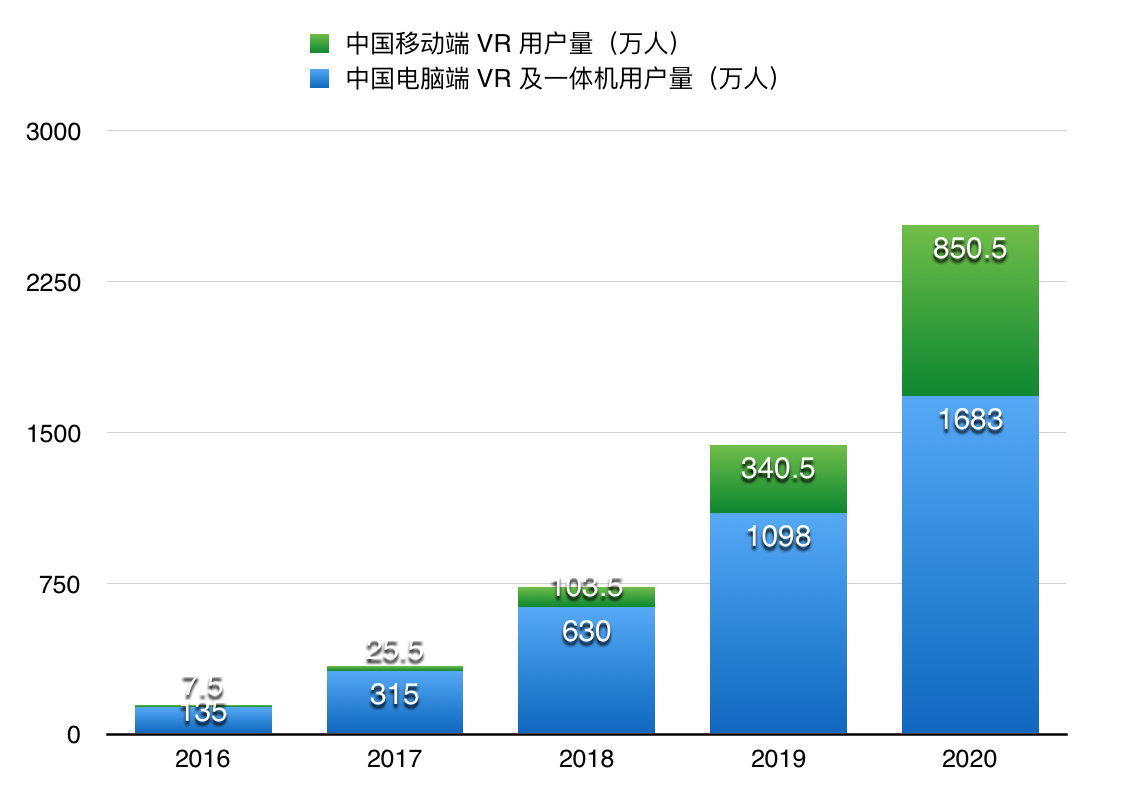
\includegraphics[width=.4\textwidth]{market}
\caption{2016-2020 年中国 VR 用户规模}
\label{fig:market}
\end{figure}

\section{全景漫游产业类别}
全景漫游产业按出发点可大体分为两类:
\begin{itemize}
	\item 以视频、游戏为主的虚拟内容提供商/平台商
	\item 涉及电商、教育、医疗、建筑等传统行业的行业融合应用服务商
\end{itemize}

短期而言,市场上比较活跃的是虚拟内容提供商,但长远而言,ToB 模式更利于产生更为健壮的全景漫游服务体系,对于高质内容的生产、分发和变现的模式也偏向于有传统大规模企业的行业服务商。

\section{全景漫游现有 APP 分析}
\subsection{Ascape}

Ascape 这款美国公司开发的应用于 2017 年发布,主攻虚拟旅游市场。你能够通过 360° 无缝的全景视频身临其境般地切身体验视频中呈现的著名景点或人文古迹,探索只有历经千难万险才能体会的绮丽风光。伴随着你的移动,场景中镜头也会随之改变整个画面的位置和显示的角度,见图\ref{fig:ascape1}。

\begin{figure}[htp]
\centering
\fbox{
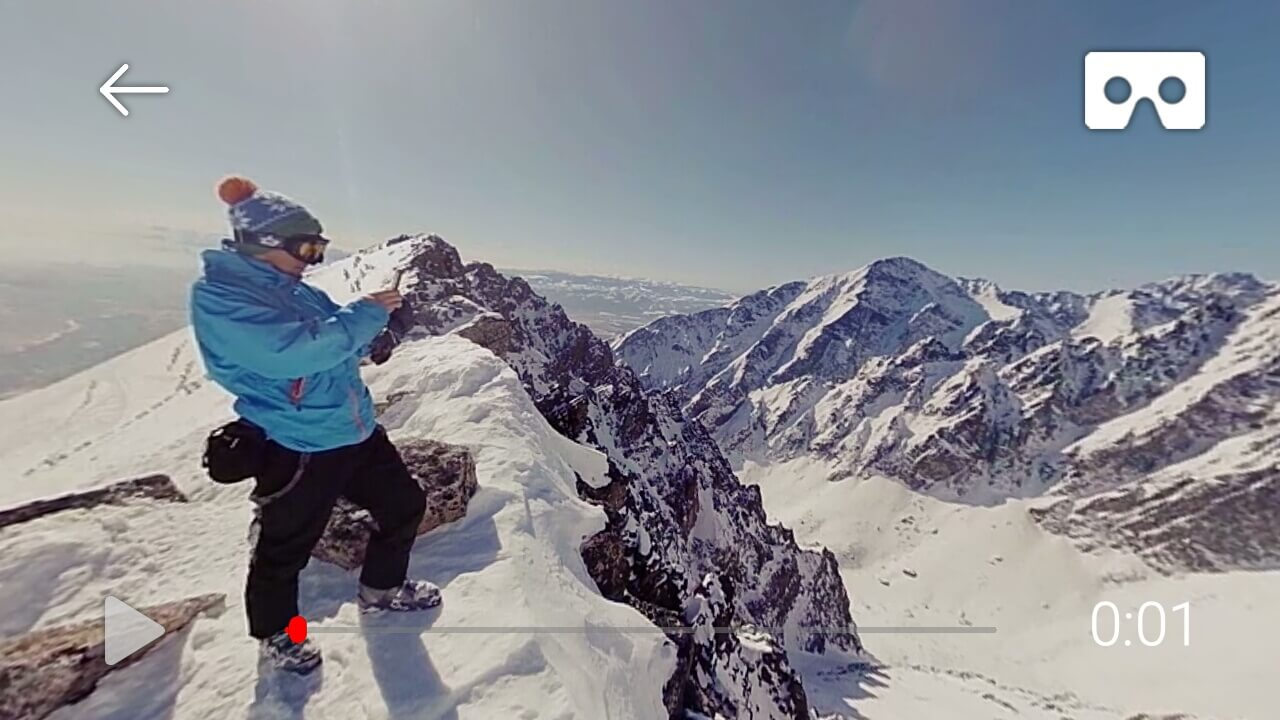
\includegraphics[width=.7\textwidth]{ascape2}
}
\caption{简洁的全景视频播放}
\label{fig:ascape1}
\end{figure}

同时,这款应用在移动应用传统界面上也继承了欧美一向以来的简约风格:“探索”页面采用卡片设计模式直观展示了新奇的场景;“发现”页面通过地图和名单两种模式展示了全球各地的场景选项;“我的旅行”也通过卡片模式展示了已下载的全景场景,见图\ref{fig:ascape2}。

\begin{figure}[htp]
\centering
\fbox{
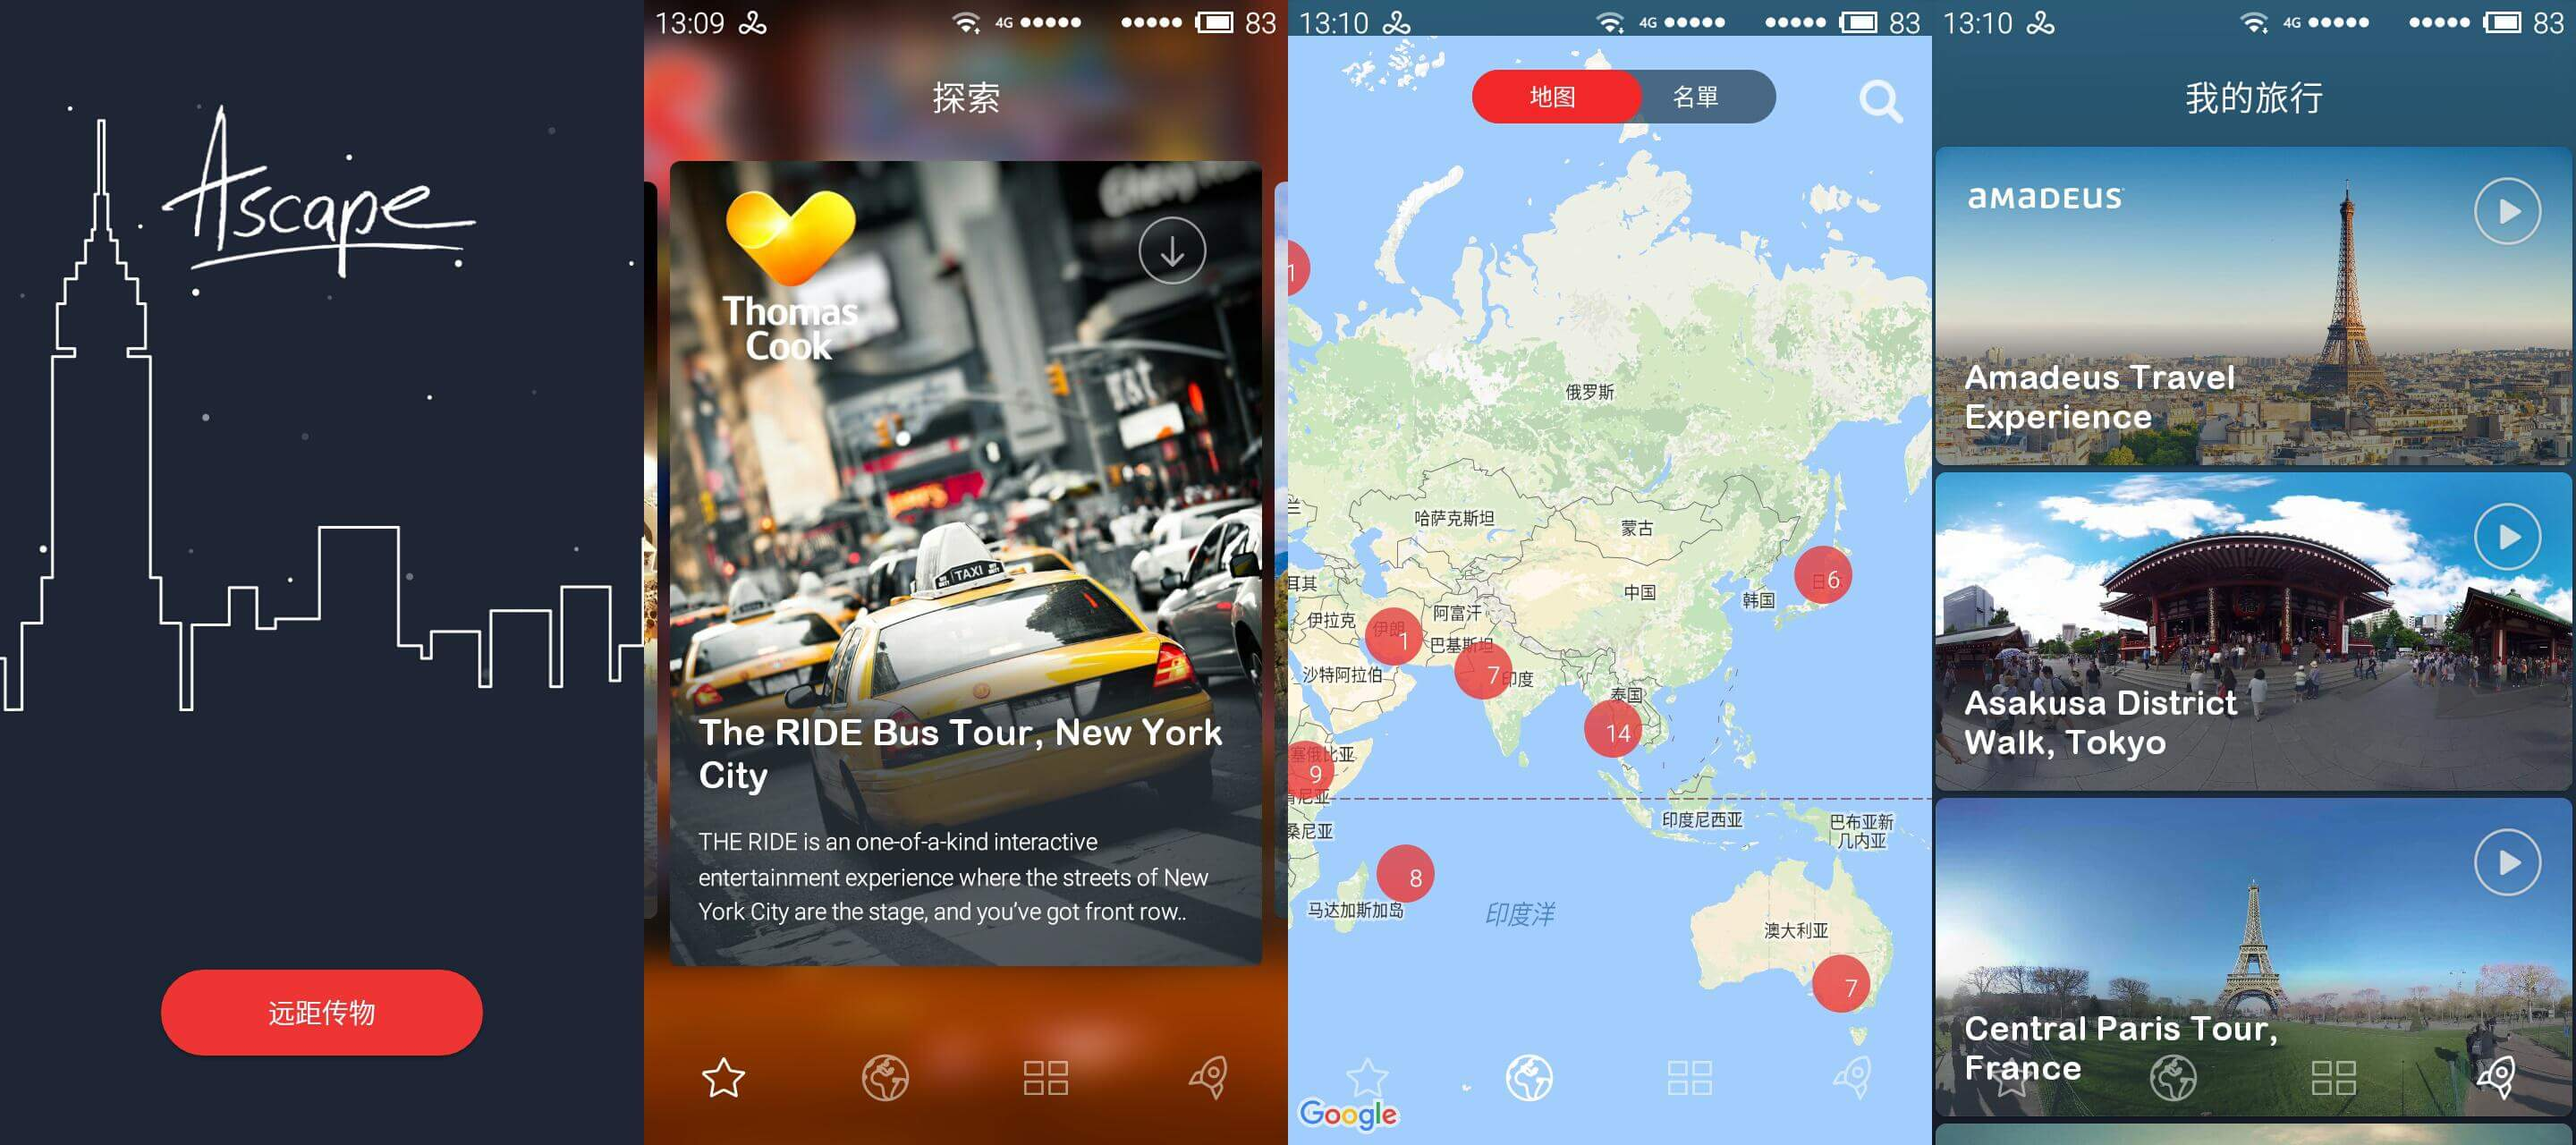
\includegraphics[width=.7\textwidth]{ascape1}
}
\caption{简洁的全景视频播放}
\label{fig:ascape2}
\end{figure}

\subsection{Fulldive}

Fulldive 这款美国公司开发的应用于 2016 年发布,是一个智能手机与虚拟场景连接的平台,进入应用后即进入了一个全景漫游的世界。场景内包含常用的网络视频、本地视频/图片、VR 相机、VR 浏览器等应用,同时支持从其内部市场下载更多基于其开发的虚拟现实应用,见图\ref{fig:fulldive1}。

\begin{figure}[htp]
\centering
\fbox{
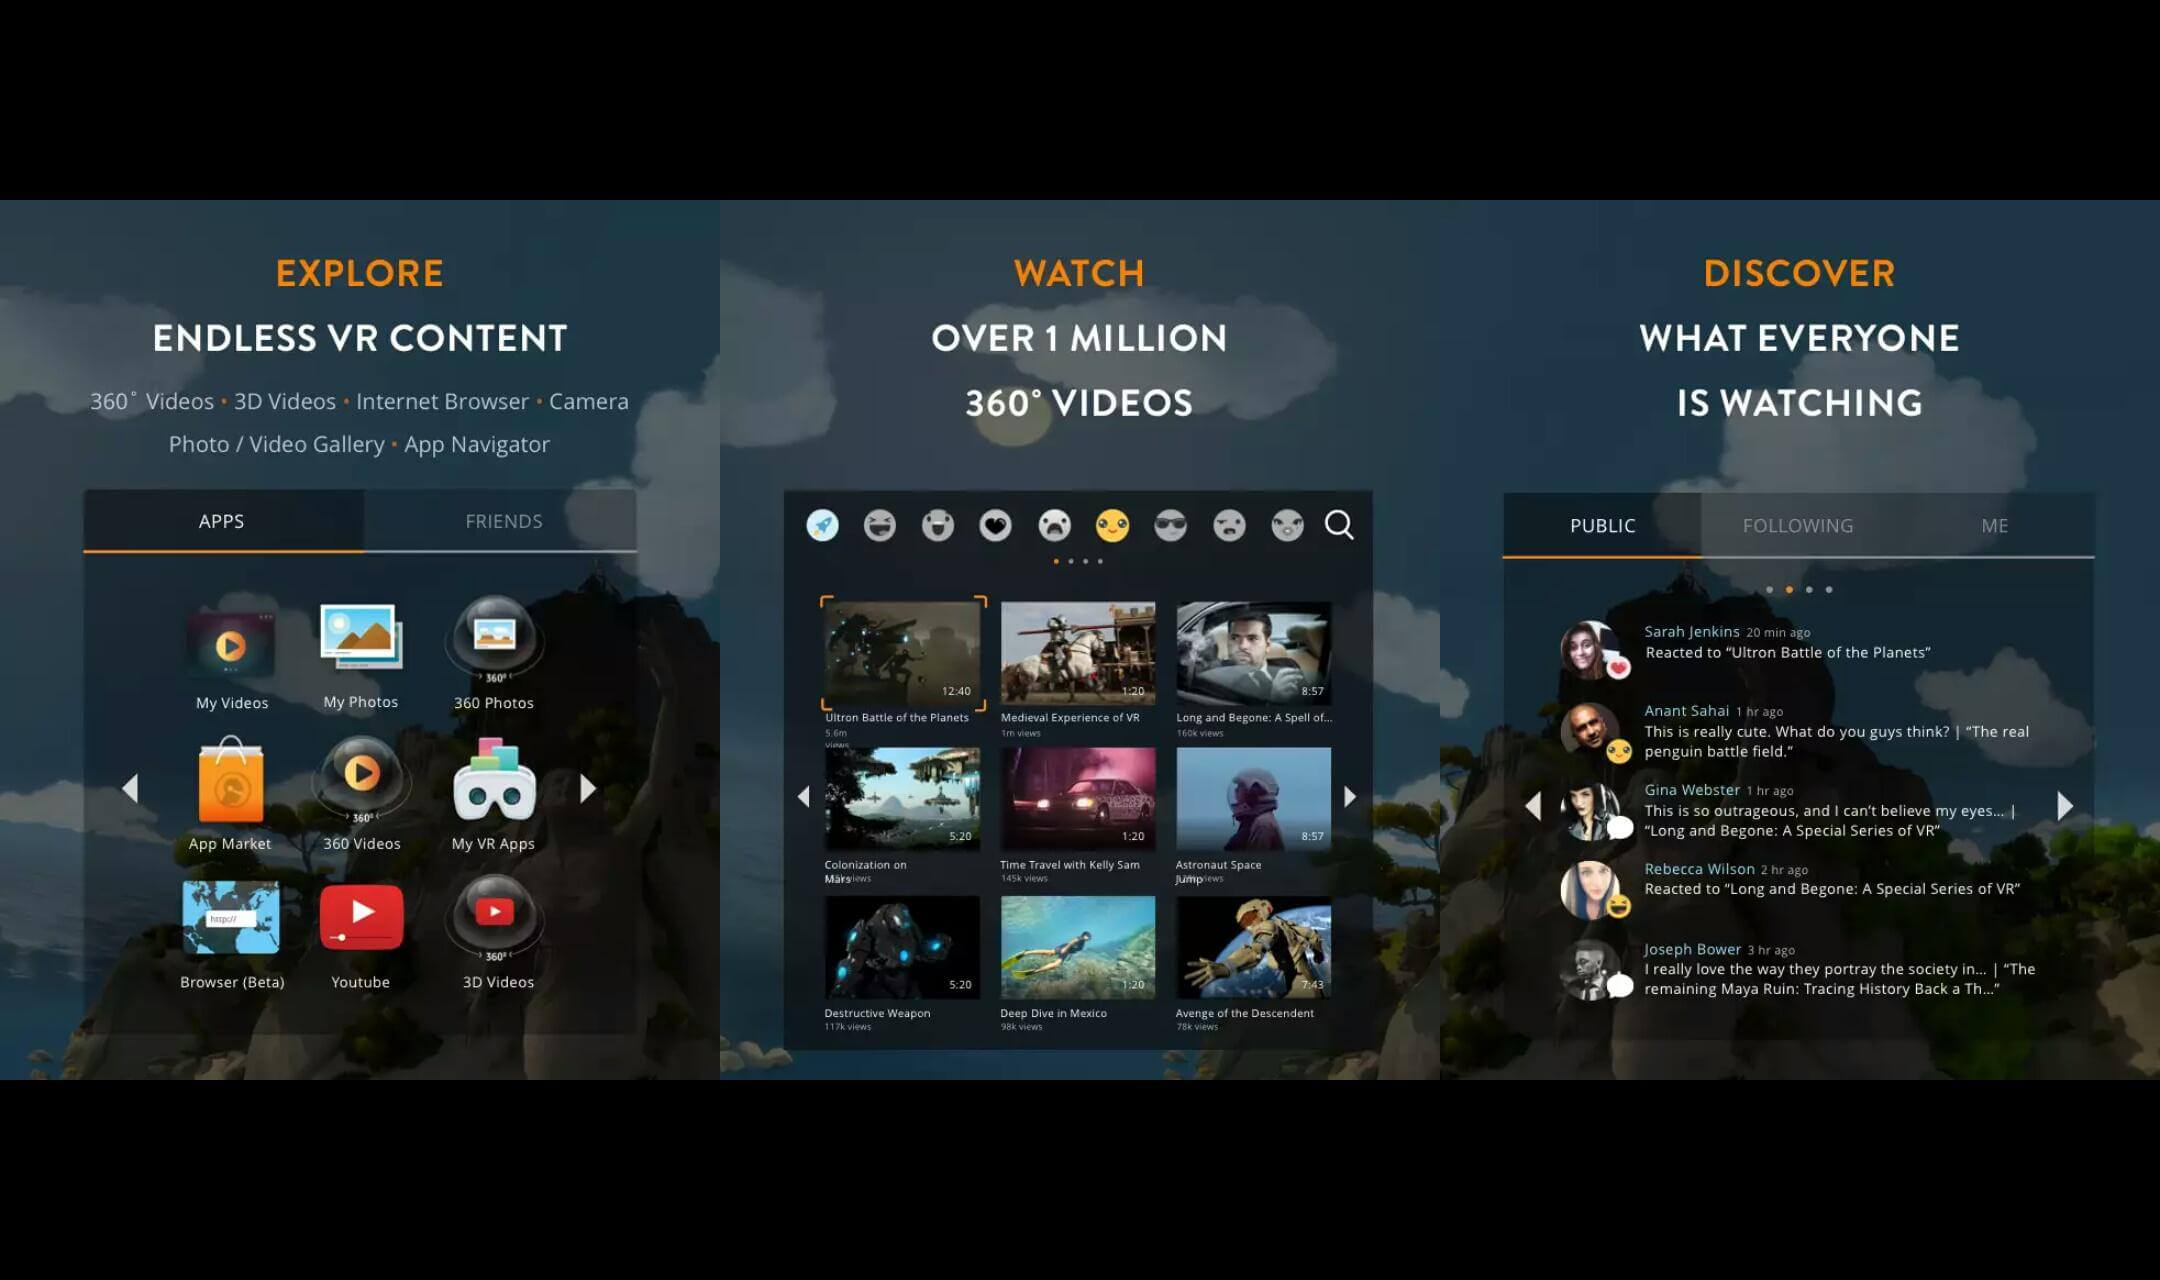
\includegraphics[width=.7\textwidth]{fulldive1}
}
\caption{Fulldive 内置的应用列表}
\label{fig:fulldive1}
\end{figure}

与 Ascape 不同之处在于 Fulldive 的操控完全是在虚拟全景中,所以在播放视频及操作选项时 Fulldive 有一些针对配戴虚拟现实眼镜者所特别提供的操作方式,见图\ref{fig:fulldive2}。例如,将视线聚焦在某个按钮上超过 3 秒后即视为按下了该按钮。这种交互形式借鉴了鼠标的双击或是触屏的长按这两种操作,同时兼顾到视线对齐对人操作的便捷性和可操作性,见图\ref{fig:fulldive3}。

\begin{figure}[htp]
\centering
\fbox{
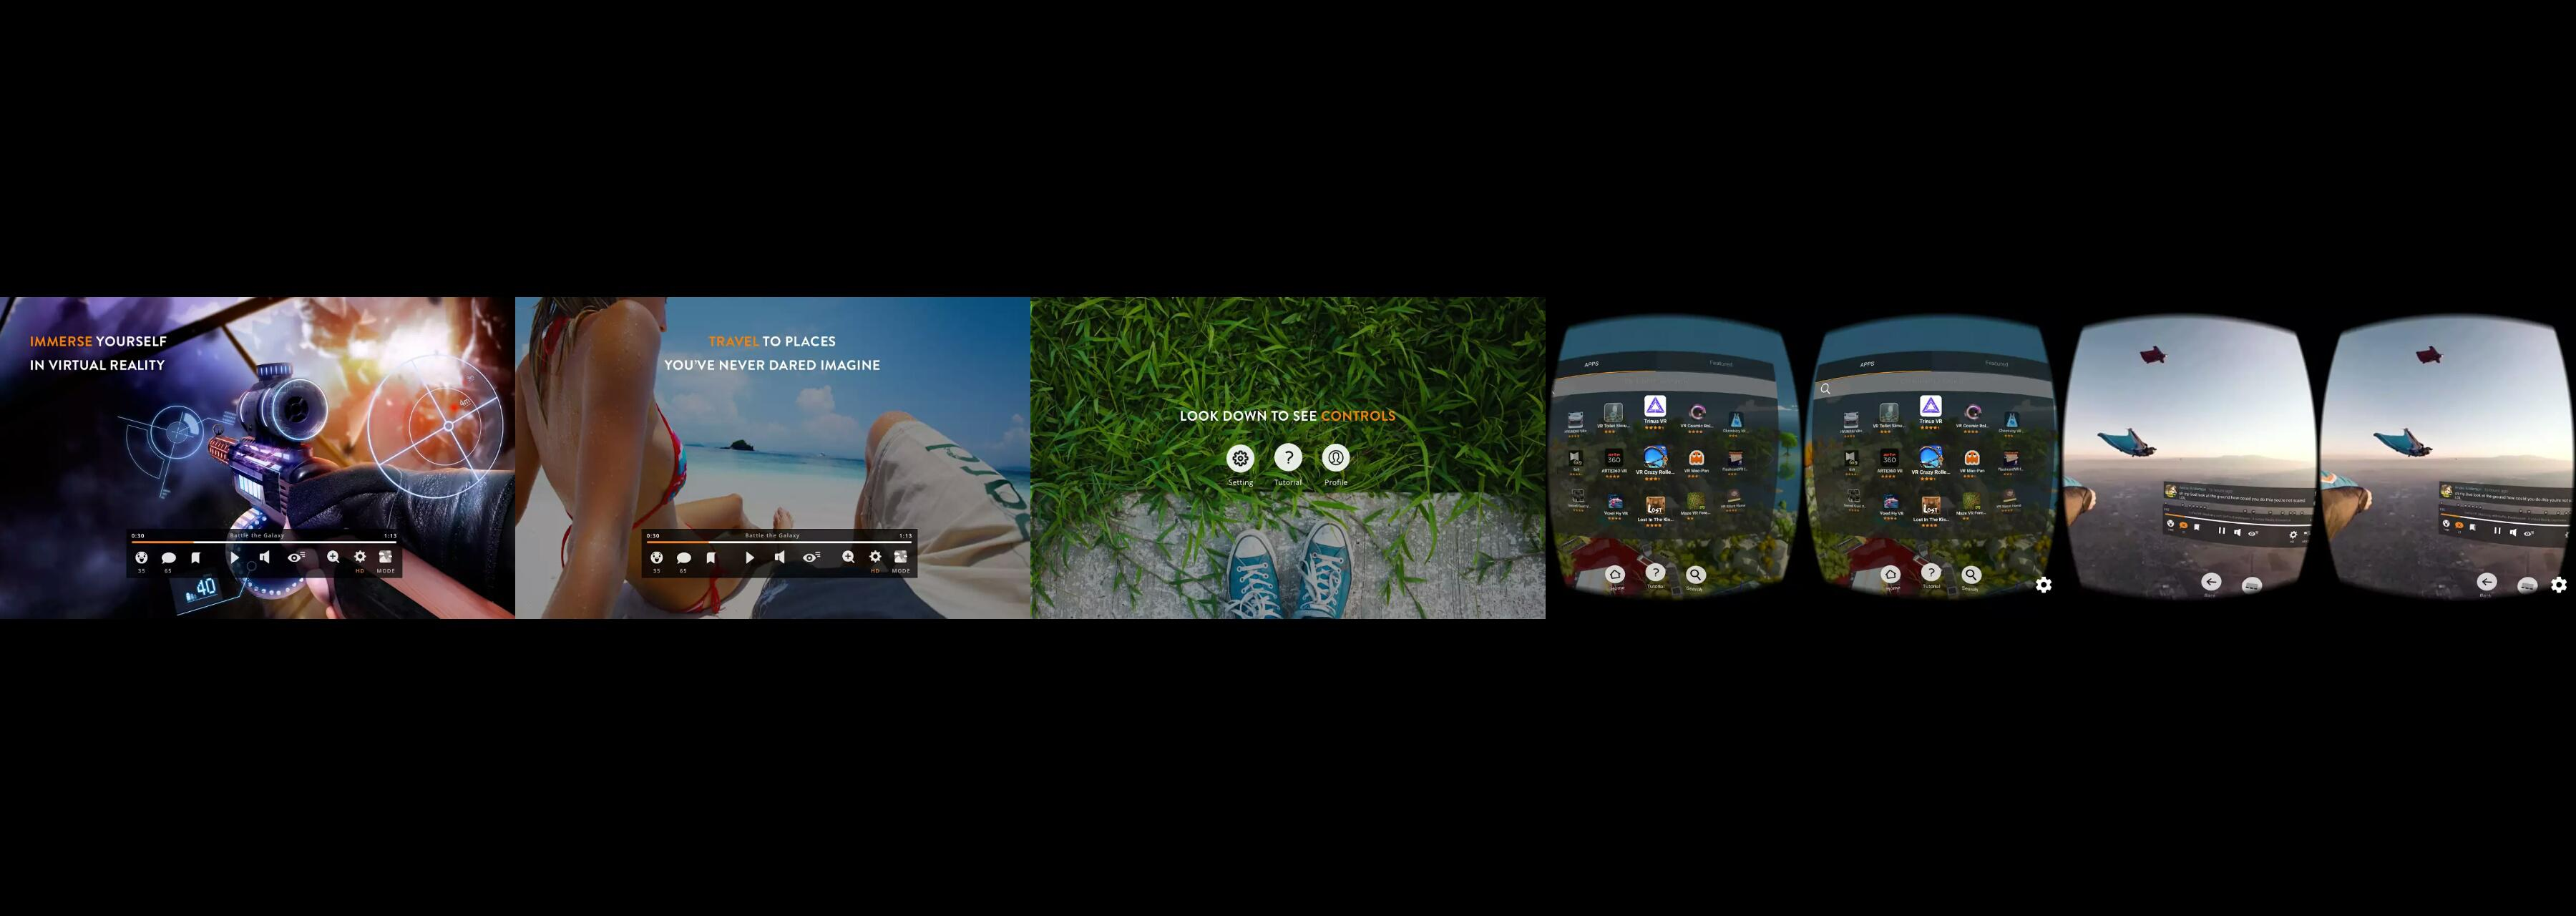
\includegraphics[width=.6\textwidth]{fulldive2}
}
\caption{Fulldive 特有操作形式}
\label{fig:fulldive2}
\end{figure}

\begin{figure}[htp]
\centering
\fbox{
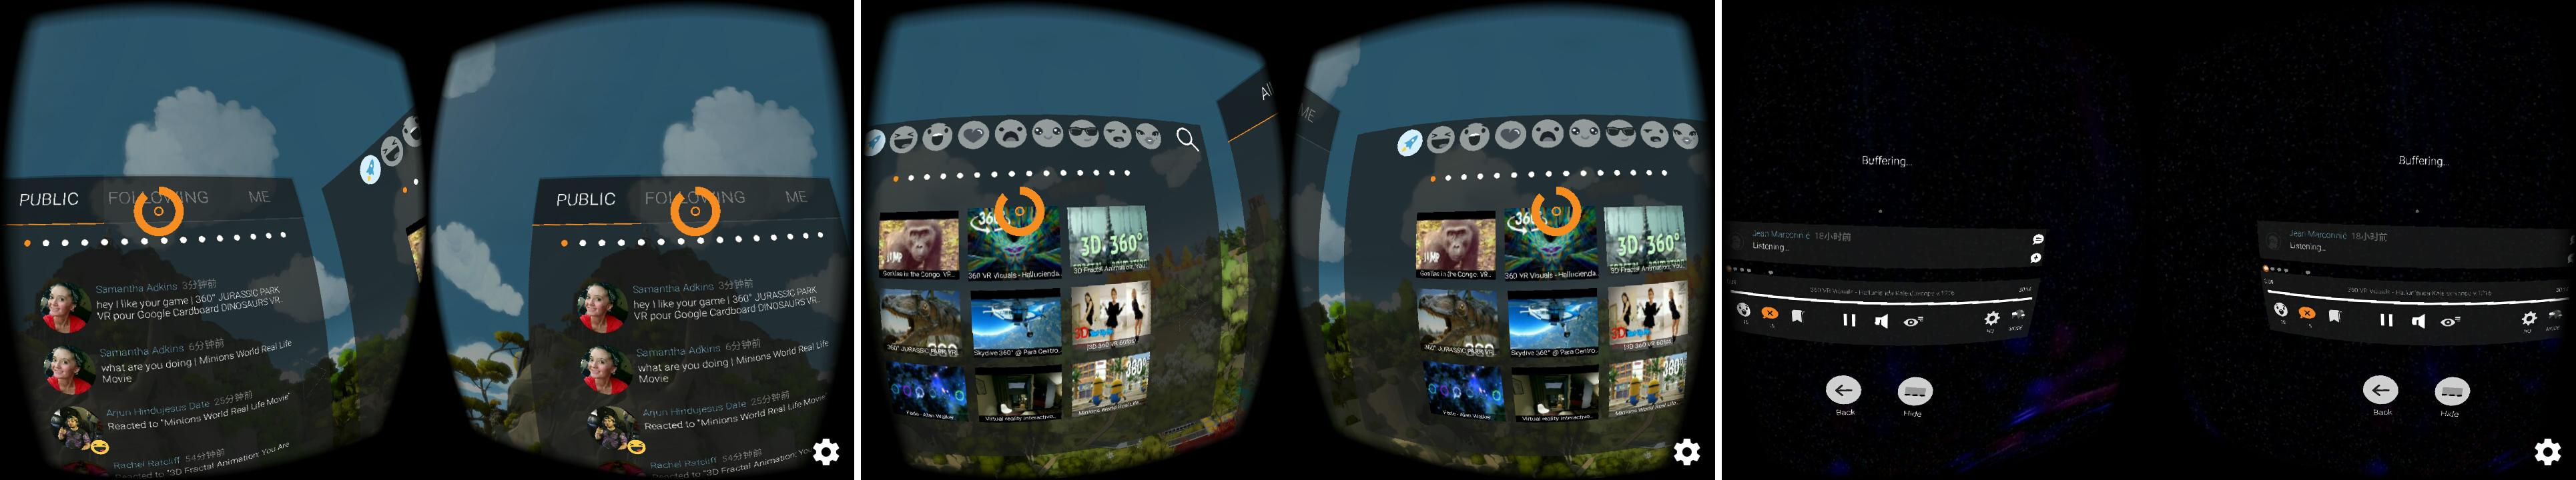
\includegraphics[width=.6\textwidth]{fulldive3}
}
\caption{Fulldive 视线停留模拟点击}
\label{fig:fulldive3}
\end{figure}

当然,这种模拟点击的操作只适用于”确认/取消“这种布尔判断的操作,用户需要输入大段的文字时则需有更高效的方式。Fulldive 结合了已日益成熟的语音识别技术,图\ref{fig:fulldive4}为实际操作 Fulldive 搜索功能并口述”中国地质大学“后的操作截屏。

\begin{figure}[htp]
\centering
\fbox{
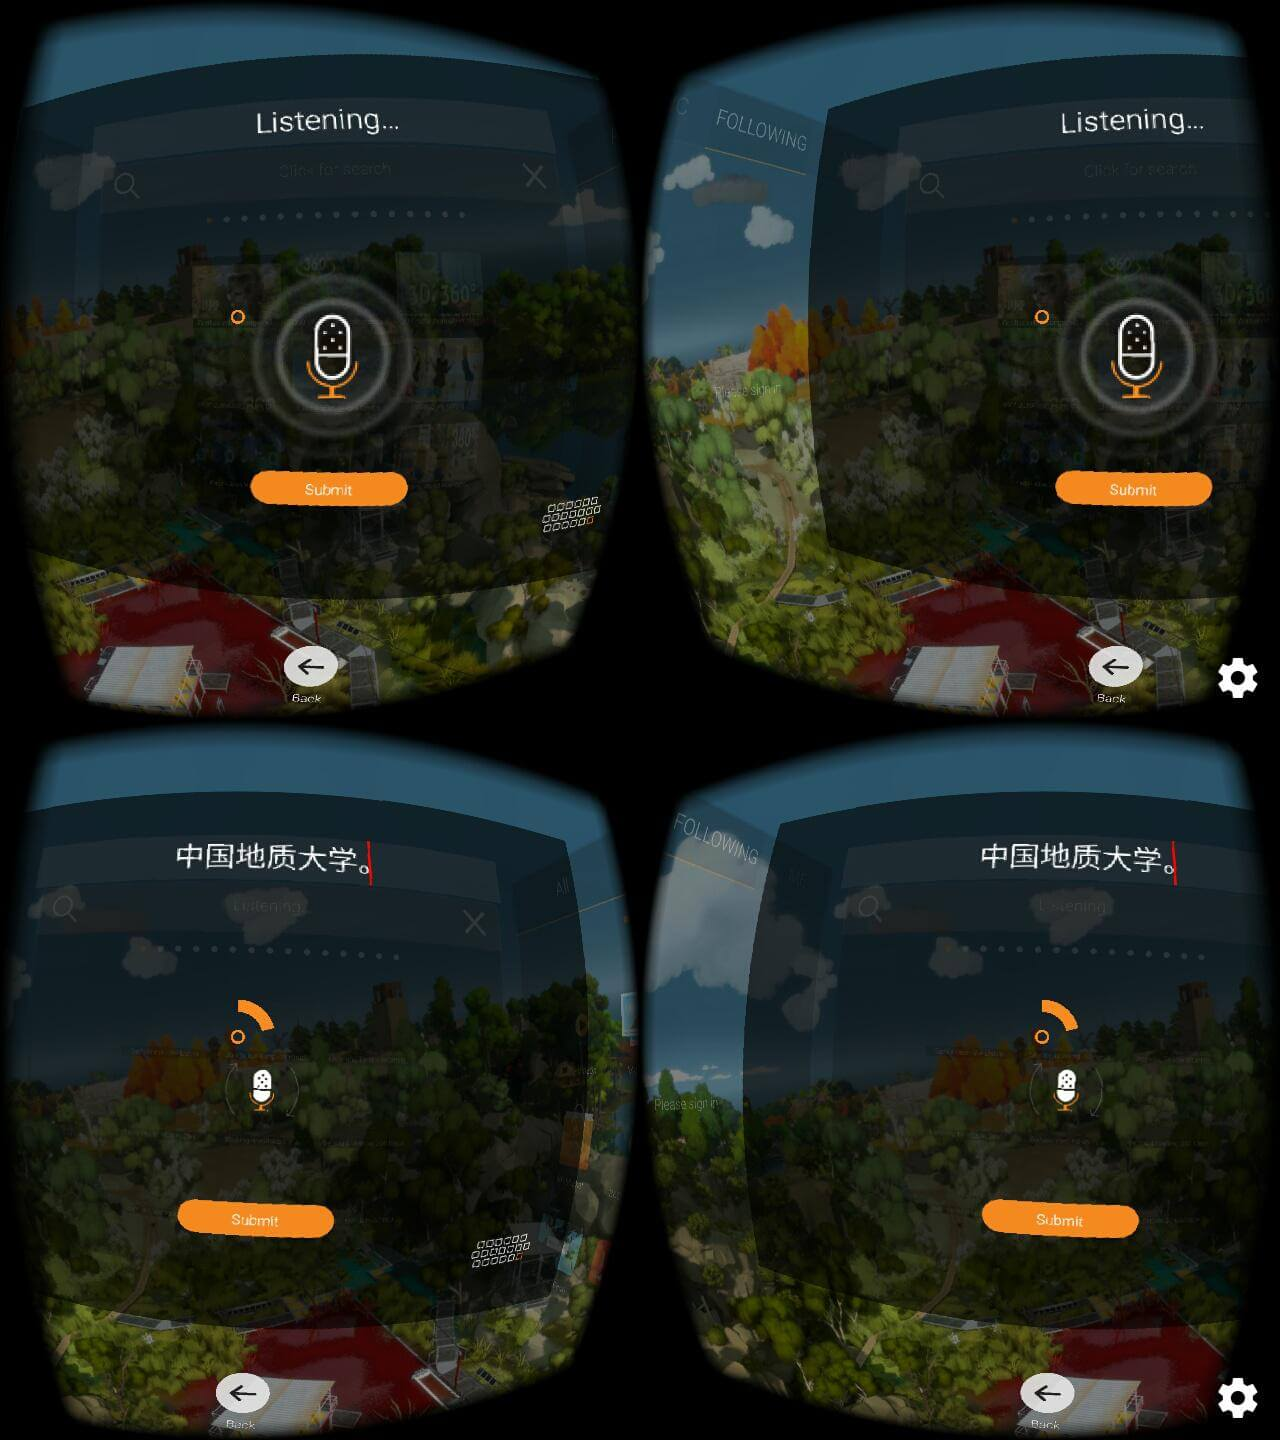
\includegraphics[width=.5\textwidth]{fulldive4}
}
\caption{Fulldive 语音识别}
\label{fig:fulldive4}
\end{figure}

\subsection{VR X-Racer}

VR X-Racer 是一款越南公司于 2016 年开发的简单的 VR 操控类飞行游戏,其操作方式为晃动设备(如 VR 眼镜或手机)来控制屏幕上的飞机躲避障碍物,见图\ref{fig:x-racer}。这是全景漫游技术在游戏上最直接的体现:几乎没有多余的操作,在游戏中飞机撞到障碍物坠毁后无操作若干秒即自动重新游戏。但其最大的缺陷是无法长时间使用,不断晃动的全景屏幕容易使人产生眩晕、恶心等不良反应。
全景漫游与 3D 影片的体验是完全不同的,全景漫游将用户完全包裹在视频所构建的封闭环境中,而 3D 眼镜只是对屏幕这种有限区域进行了折射。两者的区别在于 3D 影片由于有周围环境作为铺垫不易使人完全沉浸其中,全景漫游则是在很短的时间内(20-30 秒)就使人沉浸在虚拟世界中,直至摘掉全景设备重新适应周围环境。

\begin{figure}[htp]
\centering
\fbox{
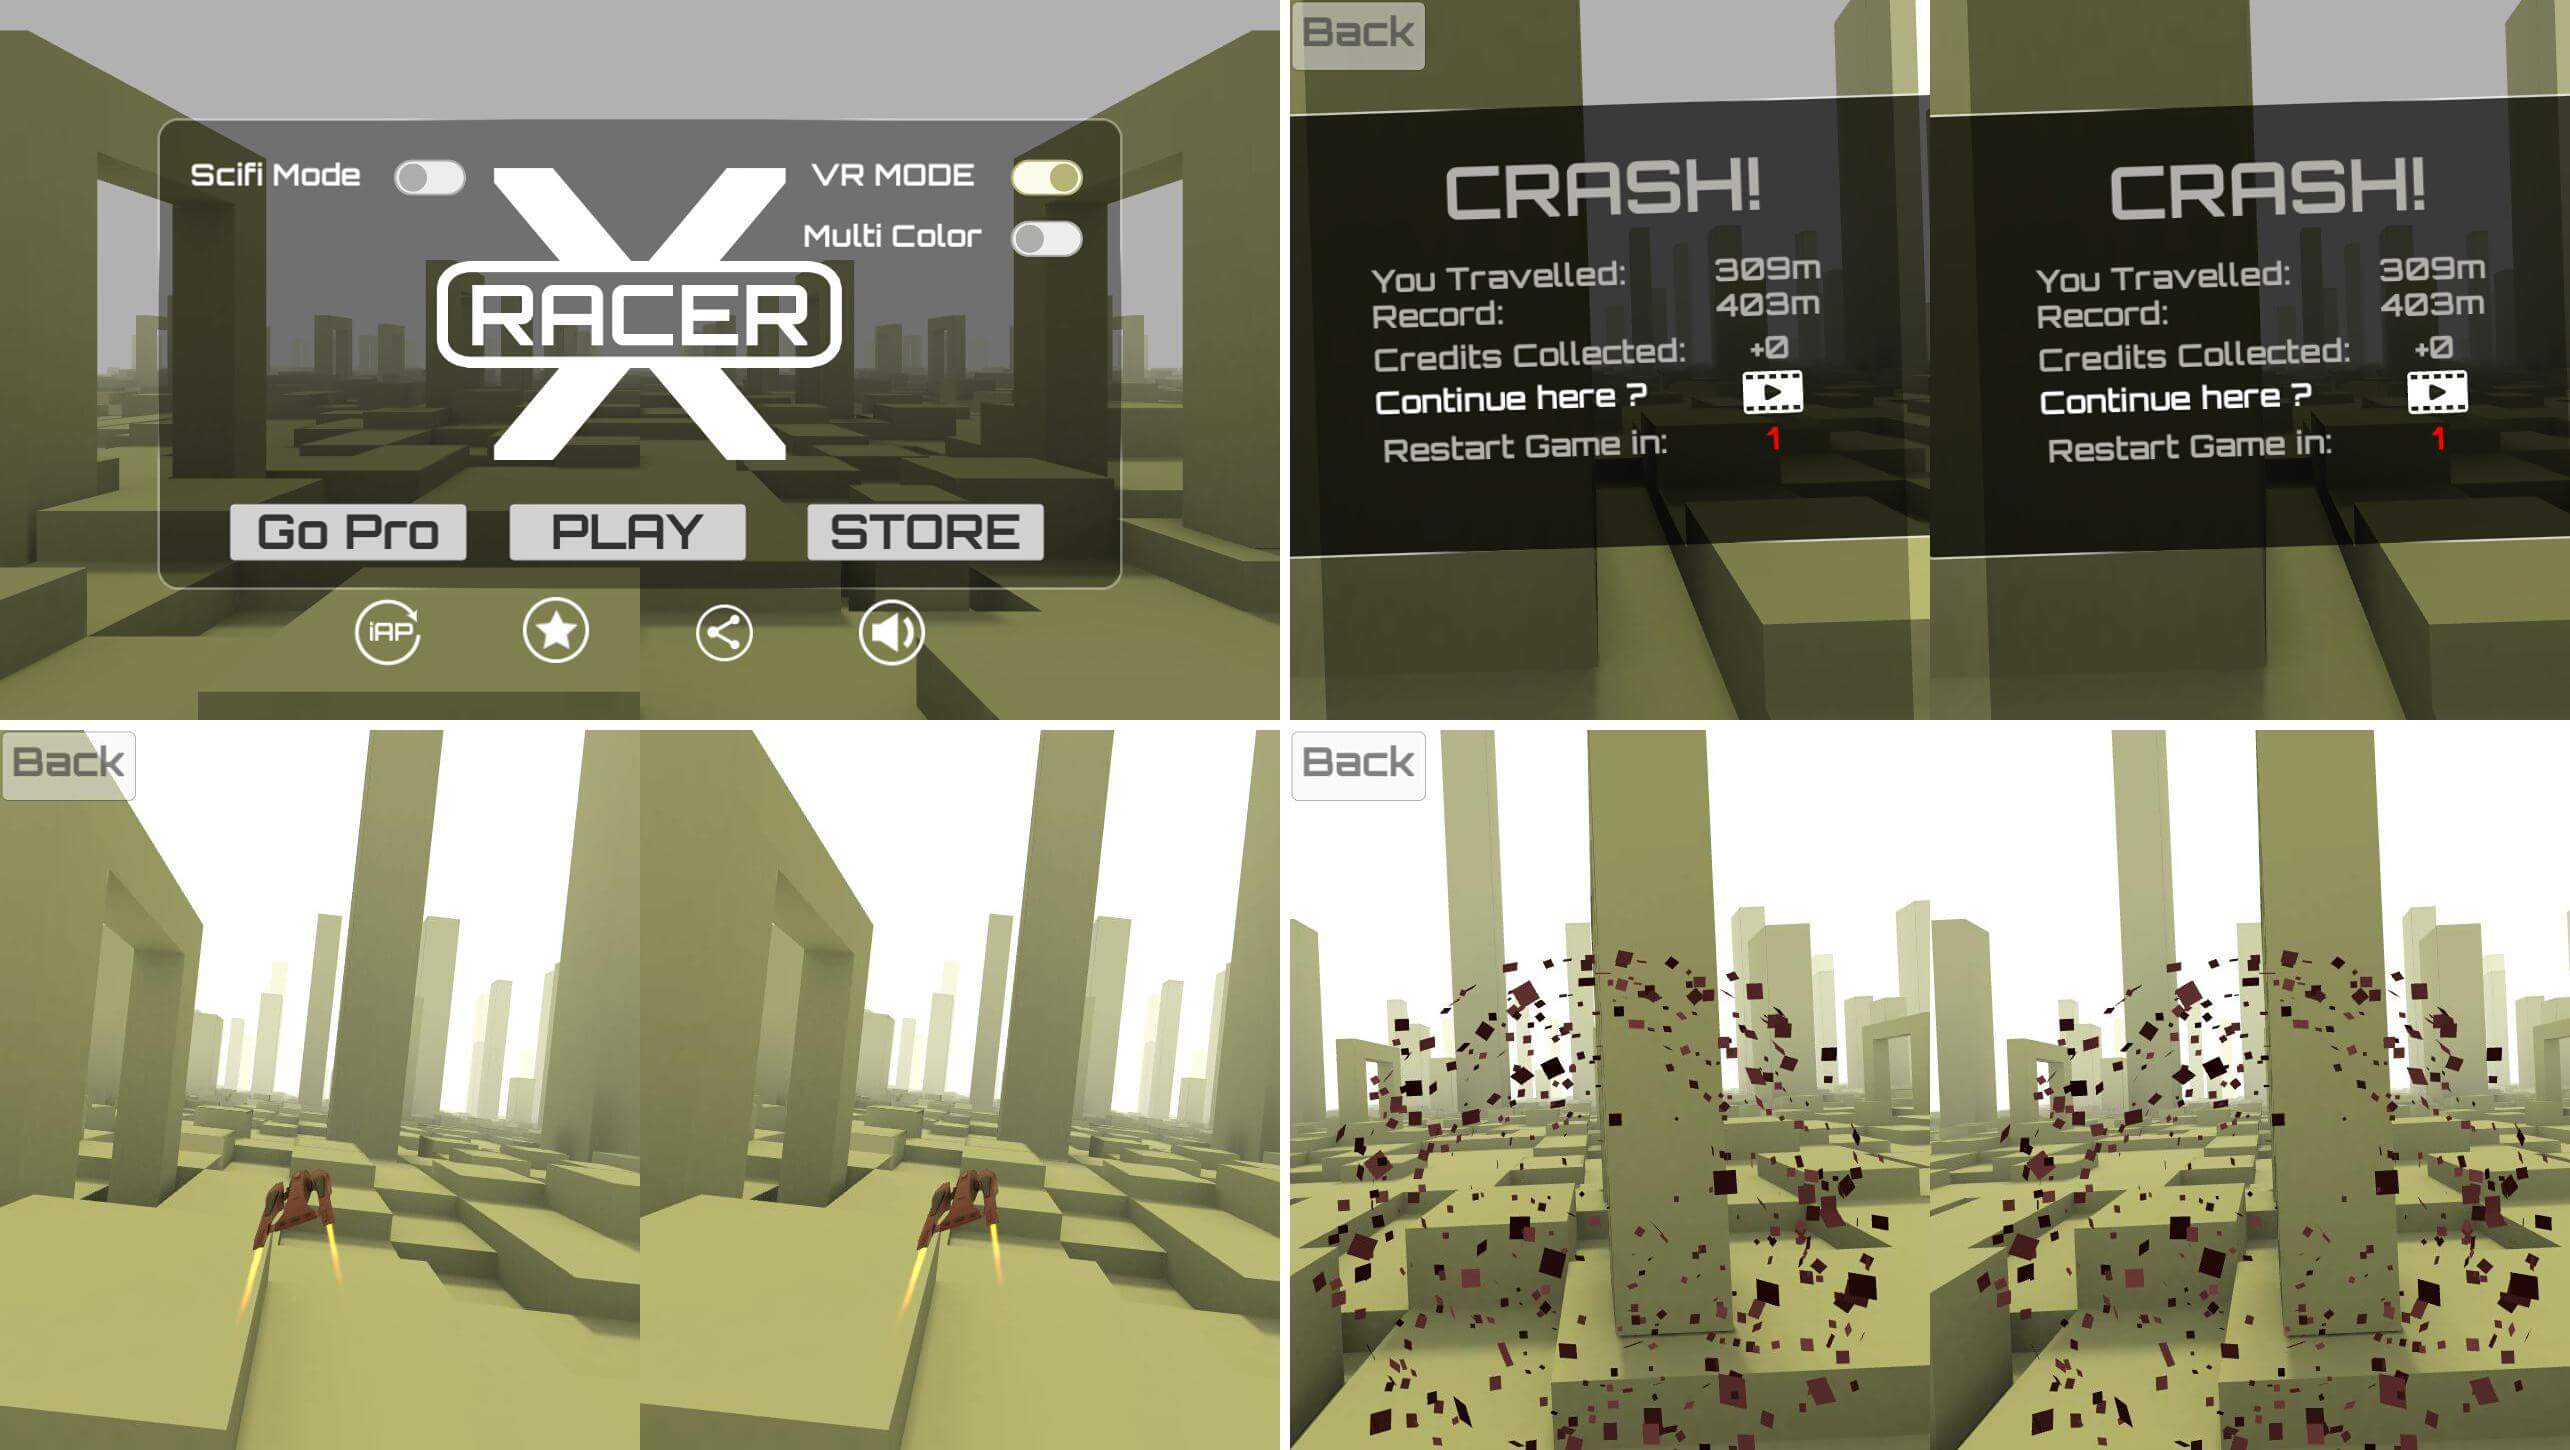
\includegraphics[width=.5\textwidth]{x-racer}
}
\caption{X-racer 游戏截图}
\label{fig:x-racer}
\end{figure}

\subsection{暴风魔镜 VR}

暴风影音是国内在全景漫游生态领域探索前沿的产品之一,最早产品发布于 2014 年,其高端产品售价可达数千元,甚至与国外高端虚拟现实设备如 Oculus 和 GearVR 等价格相齐。与其硬件设备配套的则是一款叫做“暴风魔镜 VR”的手机移动应用。

国内移动应用的发展方向一直是“大而全”,这款应用也不例外。暴风魔镜 VR 力图包括网络/本地视频、影音播放与 VR 移动应用等多种应用,形成自己的 VR 平台体系。该应用不但支持普通的移动应用界面操作模式并且同样支持全景漫游的虚拟现实体验模式。

在交互形式上与上文所列举的 Fulldive 类似,均为视线聚焦停留数秒视为确认,但缺少了语音识别输入大段文字的功能(在页面模式下支持手机输入法输入),如图\ref{fig:storm}。总体使用可满足基本的全景漫游体验,但识别速度较慢或误识别是比较严重的问题。

值得注意的一点是,暴风魔镜 VR 移动应用内场景下方有一个“归位”图标,触发后将会调整屏幕主视域至正对当前屏幕的位置,可类比于传统移动应用的“回到顶部”功能。这个功能很方便地起到了定位自身的作用,让用户不必盲目转动来寻找起始时正对着的界面。


\begin{figure}[htp]
\centering
\fbox{
  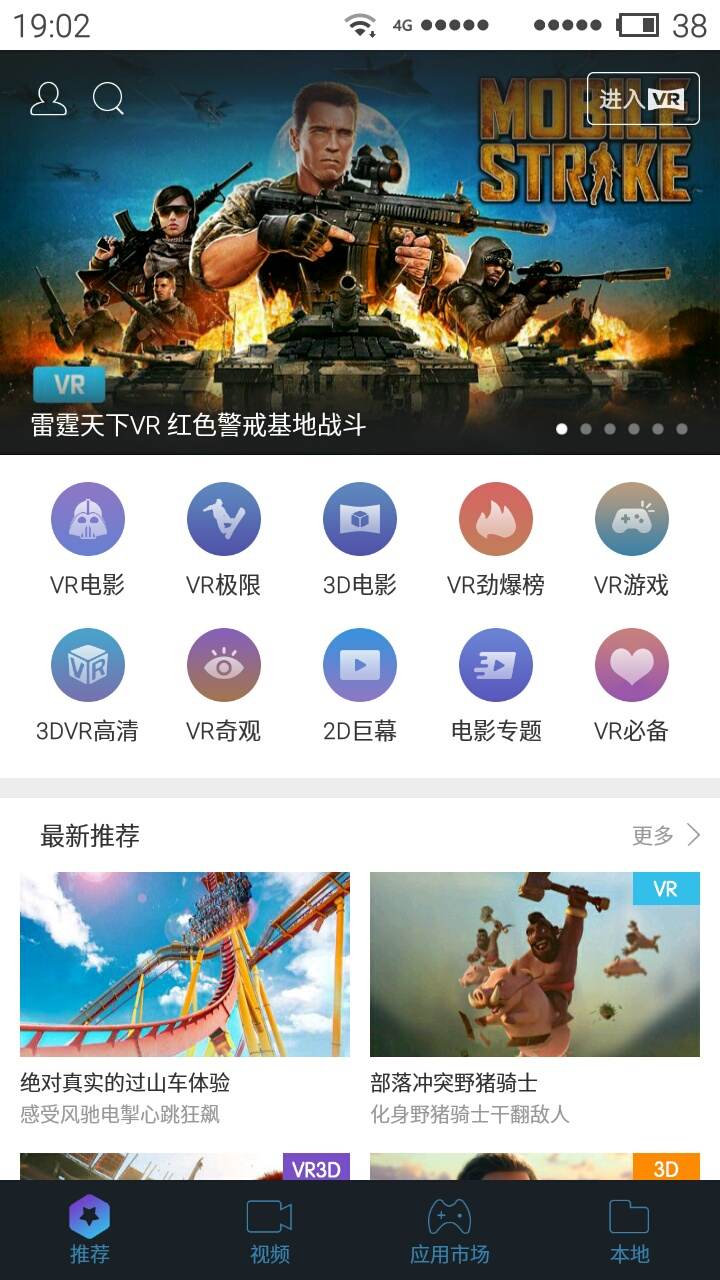
\includegraphics[width=.22\textwidth]{storm1}
}
\fbox{
  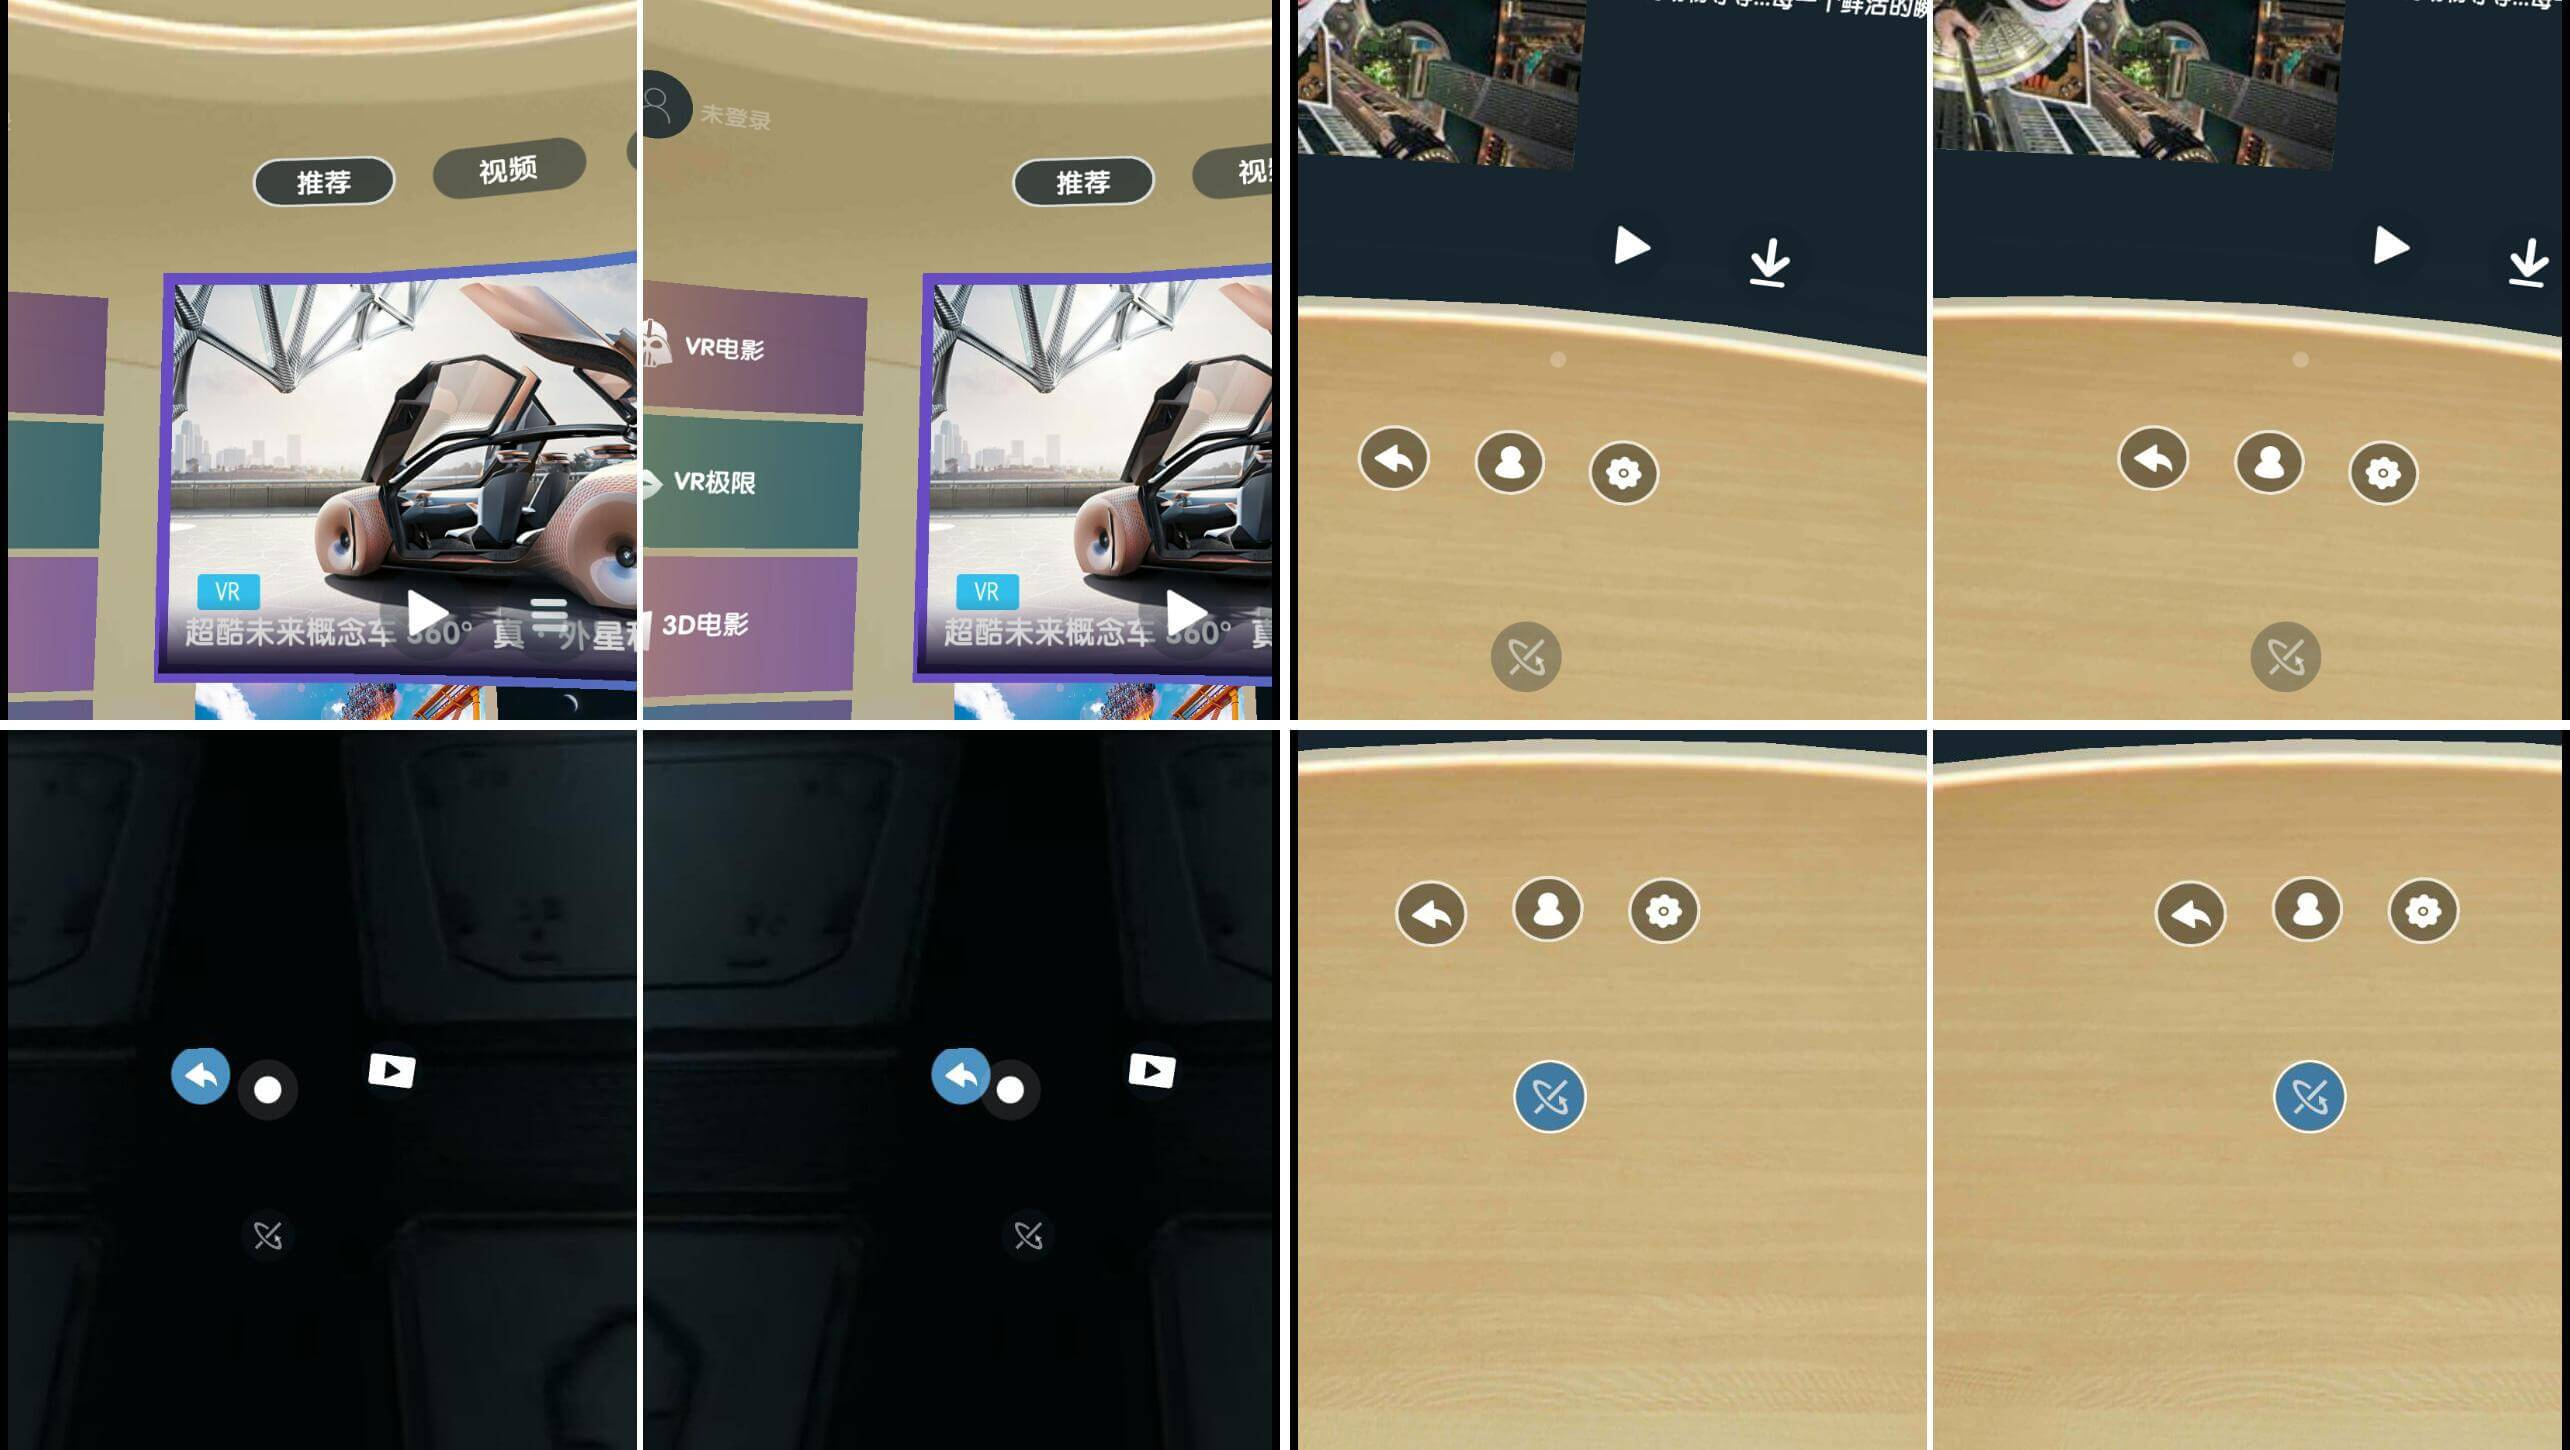
\includegraphics[width=.68\textwidth]{storm2}
}
\caption{暴风魔镜 VR 操作方式}
\label{fig:storm}
\end{figure}

\subsection{国内外移动应用总结}
国外应用较多为单一功能并凸显自身用户体验特色,而国内应用多期望建成平台式产品力图获得更大的市场份额。究其原因,国外此类开发团队小而精,立足于开发特定使用情景和目的的产品,而国内应用常常依附于配套开发的硬件设备,整体呈闭源趋势,故应用局限性较大。国外应用功能较为精简,国内应用则力图提供尽可能多的交互操作形式,但同样在交互层面难以摆脱移动设备平面屏幕所框定的范围。


\section{全景漫游行业现状总结}

全景漫游正处在行业发展的成长期,相关技术发展迅速,但同质化较为严重。众多厂商基于经济利益考量注重硬件设备的研发和更新换代,但软件质量与硬件质量仍有一定的差距,主要体现软件交互设计的质量上。

在全景漫游的交互设计上,国内外 APP 均有较多针对与不同与传统人机界面交互的创新点,例如前文列举的“视线停留数秒确定”、“语音识别”和“底部 Docker 栏”等。但交互可操作性相比于传统人机界面还有一定的差距,例如无法很快定位到所需内容、运动过程中不易操控等问题。同时,在全景漫游的现有设计中,仍旧无法脱离面向传统人机界面的设计语境,在考虑保留用户习惯的同时难以创新出更为独特的交互模式,可以说是全景漫游交互设计亟待研究的难点。

全景漫游的行业发展离不开全景漫游的软硬件及生态环境的良好结合,只有如此才能留存有效用户并产生价值,故行业目前的重点就是在软硬件上均体现出应有的价值提升。其中,软件方面可在全景漫游领域的交互方向结合相关理论作出新的设计以改善用户体验。

  \chapter{全景漫游与人的关系}

\section{全景漫游的生理行为特性}
实现全景漫游与传统人机界面最大的区别在于全景漫游时的设备(包括 VR 眼镜或专用眼罩)距离人眼只有 2~3 公分距离,设备整体对人眼呈包裹状态。使用者仅可通过听觉和其他一些不够灵敏的感觉来感受外界环境,使用环境的舒适性就变得非常重要。

全景漫游与人体关联的感觉和生理运动大致有:视觉、听觉、肢体运动等。如图\ref{fig:human_sence}。

\begin{figure}[htp]
\centering
\fbox{
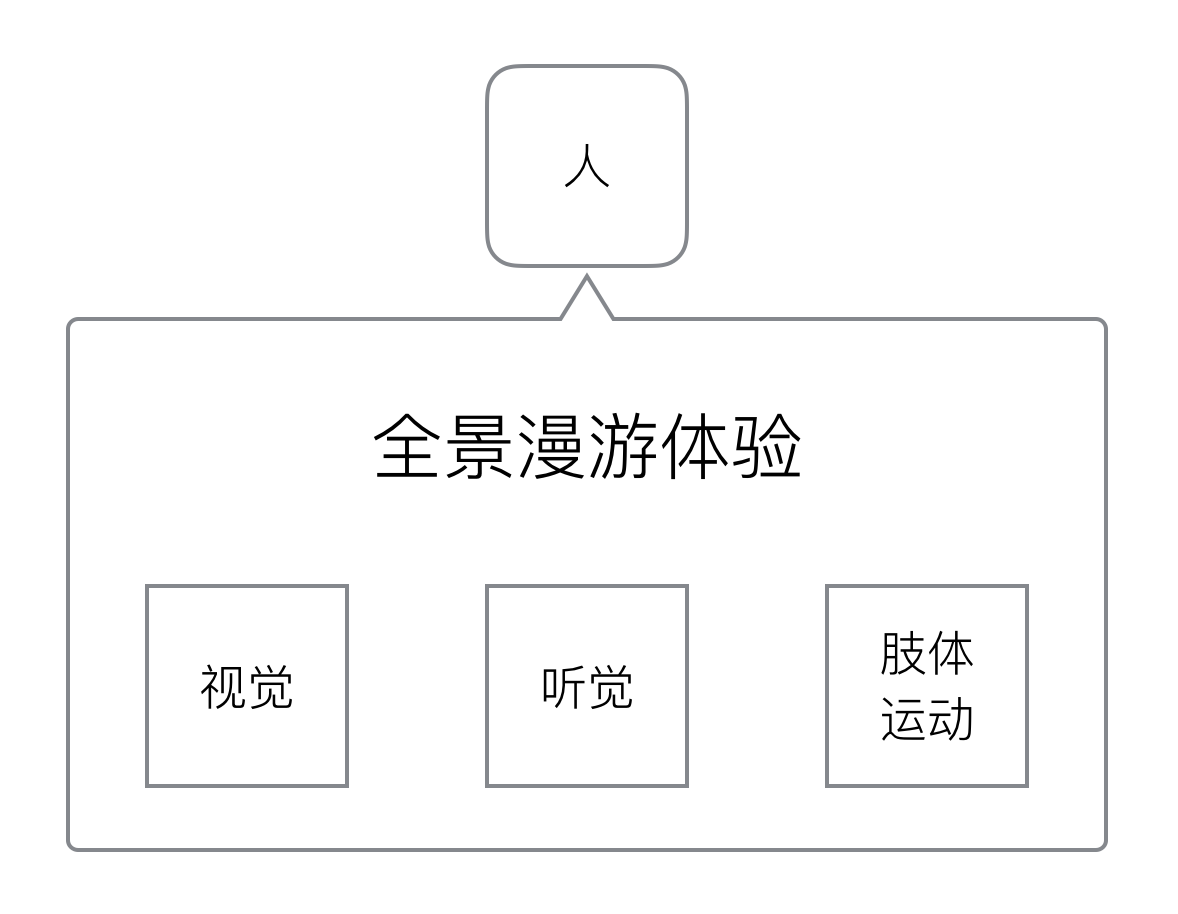
\includegraphics[width=.5\textwidth]{human_sence}
}
\caption{全景漫游与人体知觉}
\label{fig:human_sence}
\end{figure}

\subsection{全景漫游与视觉特征}
全景漫游对人体最大的刺激来源即是视觉刺激,其特征为距离眼睛距离近,色彩、明暗、动作变化等刺激较一般显示屏幕会更为剧烈。

\subsubsection{视角与视野}

人的视角是确定被看物尺寸范围的两端点光线射入眼球的相交角度。视角的大小与观察距离及被看物体上两端点的直线距离有关,其计算公式\ref{eq:angle}如下:
\begin{equation}
\alpha=2\arctan{\frac{D}{2L}}
\label{eq:angle}
\end{equation}

其中,$\alpha$ 为视角,用 $(^{\prime})$ 表示,即$(1/60)^{\circ}$单位;D 为被看物体上两端点的直线距离;L 为眼睛到被看物体的距离。
如果设眼球距镜片距离为 1.5cm,而镜片上一物体显示高度为 2cm,则带入公式可得\ref{eq:data}

\begin{equation}
\alpha=2\arctan{\frac{2cm}{2*1.5cm}}\approx 67.38 ^{\circ} = 2 \times 38.69^{\circ}
\label{eq:data}
\end{equation}

即上下视角各约为 $38.69^{\circ}$,查阅数据可知人在垂直平面的视野最大视区为视平线以上 $50^{\circ}$ 和视平线以下 $70^{\circ}$,颜色辨别界限为视平线以上 $30^{\circ}$,视平线以下 $40^{\circ}$。

由上述计算可知,在使用全景漫游设备观看场景时,假设高为 2cm 的显示物体在人视野中上部已超出颜色辨别界限,下部也已接近颜色辨别界限。物体上部比下部更接近垂直平面内的视野极限,如图\ref{fig:angle}。由此可知,全景漫游场景设计中应将主要元素置于屏幕中央,次要元素尽可能置于屏幕下方以便识别操作。同时,色彩丰富且饱和度高的元素也应置于视野中部,而一些操作类的元素则不应用过于丰富饱和的色彩缀饰,以免让使用者应难以分辨色彩而操作出错。

\begin{figure}[htp]
\centering
\fbox{
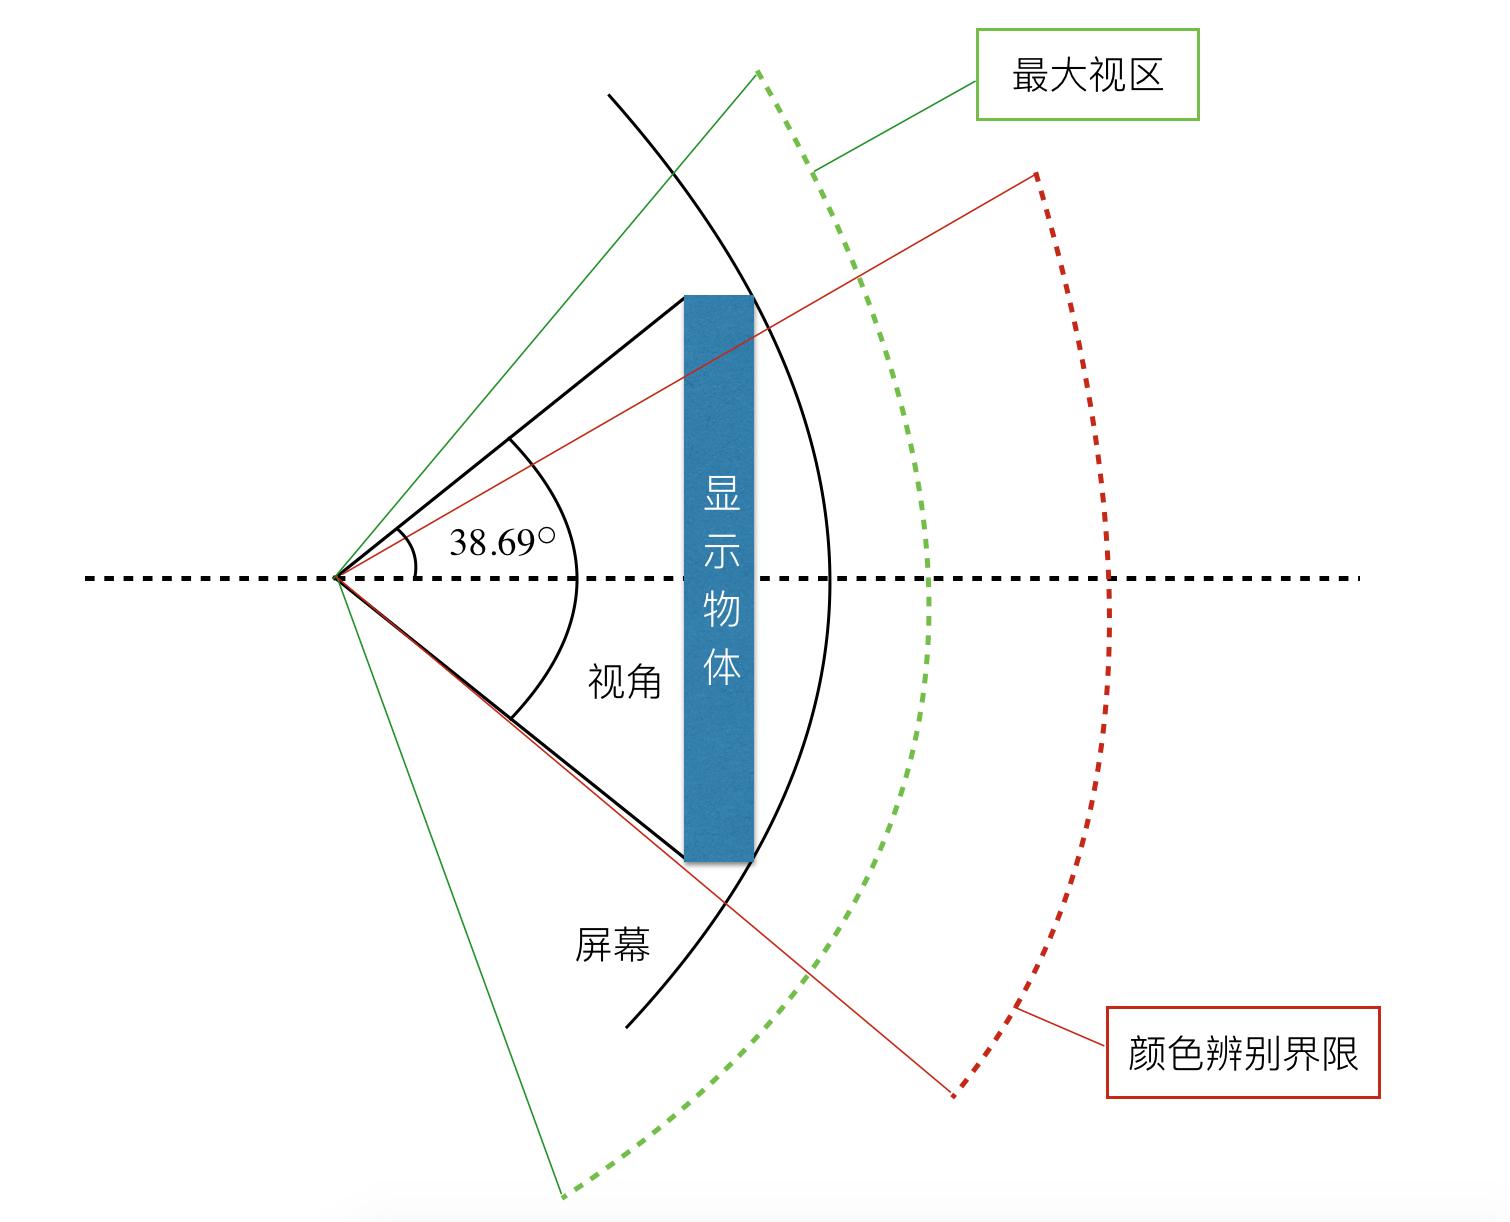
\includegraphics[width=.7\textwidth]{angle}
}
\caption{全景漫游中视野的角度关系}
\label{fig:angle}
\end{figure}

\subsubsection{视觉适应}

配戴全景漫游设备进行观察时,屏幕距眼球距离不足 2cm,属于视距过近状态,应当避免长时间操作,否则易引起眼睛疲劳。同时由于屏幕与眼球距离过近,屏幕亮暗对眼球刺激比通常工作环境更为强烈。当屏幕上场景切换间明暗变化过快时,人眼需要一定的适应时间才能正常分辨,但由于全景漫游设备等封闭性,无法较轻易地脱离这种明暗急剧变化的环境,则眼睛无法得到充足有效的适应时间,则很容易产生视觉疲劳,影响视觉能力。

\subsection{全景漫游与听觉特征}

全景漫游的视觉是主要人体感觉,但听觉是仅此于视觉的重要感觉,尤其是在视觉被全景场景完全包裹住的情况下。

现有全景漫游设备有的自带耳机设备,也有的需要自行配备耳机。但长远来看,配备耳机可能是必然的选择。因为人耳具有“方向敏感度”(或称“双耳效应”),即:声波在进入鼓膜时,受人体的反射、折射和衍射而扭曲变形,大脑能根据经验判断出声源的方位和距离。而前文所说的“耳听八方”即说的是这种能够重建场景音效的能力。

\subsubsection{双耳效应}
为了“制造”出能够“蒙骗”大脑使其误以为使用者身处虚拟场景中的体验,大致方向是重建出空间任意一点至双耳处的滤波器函数。我们不必去关心空间中某一点的声波是如何传播到人耳中的,只需要将该点声波信号经过滤波器便可以得到它在人耳处的声波信号,如图\ref{fig:hrtf}。而这个信号是可逆的,即被人耳捕捉到之后便由大脑还原成相应位置的“声信号”,从而达到“欺骗”大脑的目的。这个领域的研究对象叫做 HRTF(Head Related Transfer Function):头相关变换函数,是一种音效定位算法。但每个人的听觉能力都是不同的,所以 HRTF 对人类整体并没有通解,而只有对于人类个体经过反复实验测试后的特解。

\begin{figure}[htp]
\centering
\fbox{
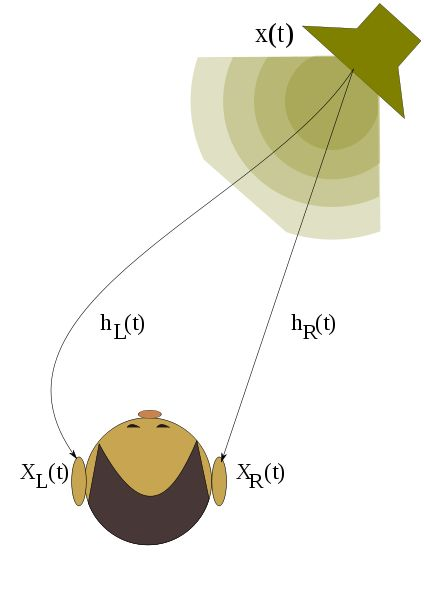
\includegraphics[width=.4\textwidth]{hrtf}
}
\caption{头相关变换函数 HRTF}
\label{fig:hrtf}
\end{figure}

国内外已有厂商根据相关理论设计并制作出了 VR 耳机,可配合 VR 眼镜使用,也可独立使用,它会追踪使用者的姿态、位置变化等,进而计算并还原出模拟三维场景内的声音分布,让使用者仿佛置于真实的场景之中。

\subsubsection{视觉的「补充」}
虽然声音不是可视化领域的研究重点,但良好的听觉体验的确有利于信息渠道的建立。视觉与听觉互为补充、相互作用、最终是人的知觉更为敏锐而准确。可以设想以下场景:「用户配戴全景漫游头盔进行一场探险类的游戏,用户扮演的主人公正在探索未知的世界,正当主人公小心翼翼地穿过一片沼泽时,后方突然传来了一声尖叫…… 」如图\ref{fig:audio-source}看不见的事物通过音效来表现,可以提升场景所渲染出的气氛效果。听觉与视觉不同,不受方向影响,能够用来表现一些视觉上无法做到的特殊效果。

\begin{figure}[htp]
\centering
\fbox{
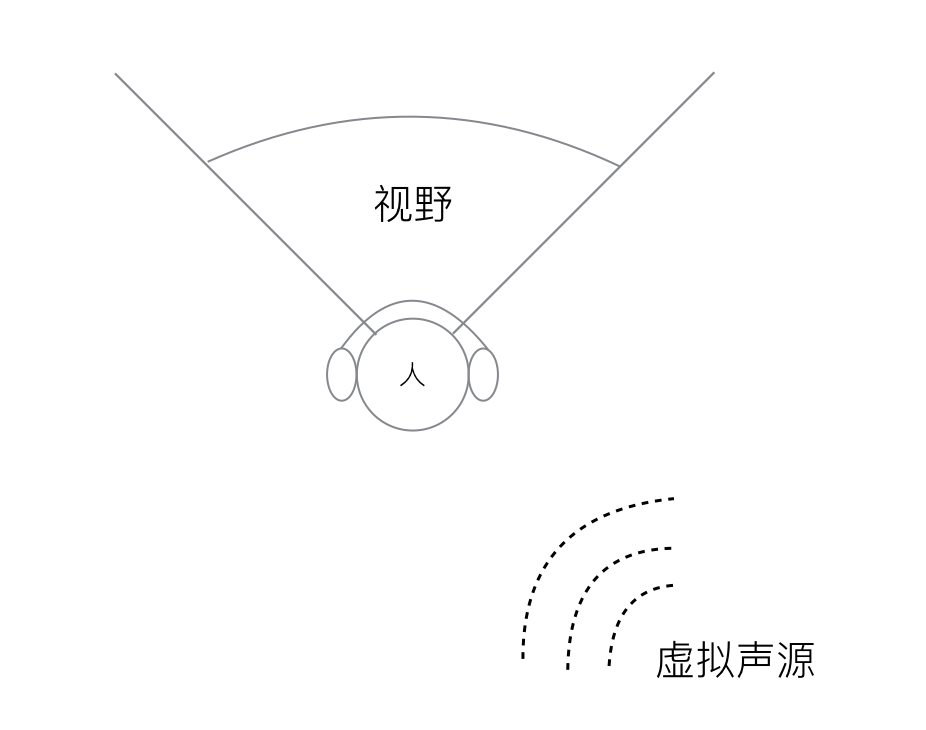
\includegraphics[width=.5\textwidth]{audio-source}
}
\caption{用音效来表现「看不见」的事物}
\label{fig:audio-source}
\end{figure}

\section{全景漫游与肢体动作}

全景漫游,其一是“全景”,其二则是“漫游”。漫游,意为随意游玩、漫无目的地行走。全景漫游的体验重在参与感的营造,用户不仅能够“身临其境”般地体验全景场景,更可以亲身参与其中,与场景中的虚拟事物进行互动。

\subsection{平衡感}
众所周知的是,人之所以可以站立行走、骑行脚踏车或进行高空作业依赖的是人与生俱来并在后天不断磨合的平衡感。平衡感由内耳的淋巴液控制,同视觉相互配合,使人能安全地四处走动。而在全景漫游过程中,人的视觉几乎全部集中在眼前的屏幕上,即很难看到外界真实的场景,故视觉此时便难以匹配内耳中内淋巴液流动引起的细胞兴奋,对人来说就是平衡感的缺失。失去平衡感会使人晕眩,严重时会使人倾倒,有造成意外伤害的可能,故在进行全景漫游时应尽可能减少乃至避免对平衡感造成的影响。

维持平衡感有两种方式,一种是降低运动的速率(即减小在全景漫游中需要运动的强度)视为主动维持平衡感,另一种是通过某些手段来减少视觉或其他感觉中平衡感的减少,即运动补偿,可视为被动维持平衡感。

现有全景漫游设备部分带有陀螺仪、部分利用手机内置陀螺仪用以感应方位信息,可做运动补偿以模拟人在环境中的运动,但人的眼球可以根据平衡来进行前庭—眼动反射 ( vestibulo-ocular reflex)控制眼球作补偿性运动,使之匹配头部的转向,以求维持人视野的稳定。这套机制在不戴全景漫游设备时可以正常运作,但在配戴了全景漫游设备后因眼镜视野与外界隔离,故设备与外界的运动匹配度就变得格外关键。

现有普通手机所内置的是微机电陀螺仪(MEMS),是利用物理学的科里奥利力,在内部产生微小的电容变化,通过测量电容,计算出角速度,从而判断物体转向和速度,这种芯片价格低廉,体积小巧,但缺点是因其电磁特性易受环境干扰,而且精度即使能够满足一般手机应用(如转屏、翻转等)但在更为精细的全景漫游的方位感应上还是显得力不从心。屏幕显示画面本身就有约 1/60s 即 16ms 左右的刷新时差,再加上陀螺仪反馈信息与实时状态也有偏差,两者累积后在使用者运动时画面很难及时更新至准确的位置上,容易造成失去平衡的感觉。甚至在人停止运动后,全景漫游设备错误地输出带有运动补偿的画面以致人眼误以为人体还在做运动,造成认知上的偏差,导致非运动状态下的感官刺激,这种刺激往往对使用者造成较长时间的影响,延续到使用完全景设备后的数分钟乃至若干小时后。

全景漫游技术的发展在维持人体平衡感方面尚有很大的发展空间,现有高端全景漫游设备即使是支持全方向漫游的平台也只允许使用者慢步使用,而运动补偿机制仍沿用着手机等终端的设计(大多数全景漫游设备并没有自己的陀螺仪,而是直接调取了与其连接的手机的重力感应接口)在需要高精度分辨的场合表现就达不到使用要求了。

\subsection{关节运动}

全景漫游人体主要运动可分解为躯干的平面运动和头部的转动,这两方面配合眼球的转动就构成了全景漫游中人个体在场景中的位移和转向,如图\ref{fig:act}。

\begin{figure}[htp]
\centering
\fbox{
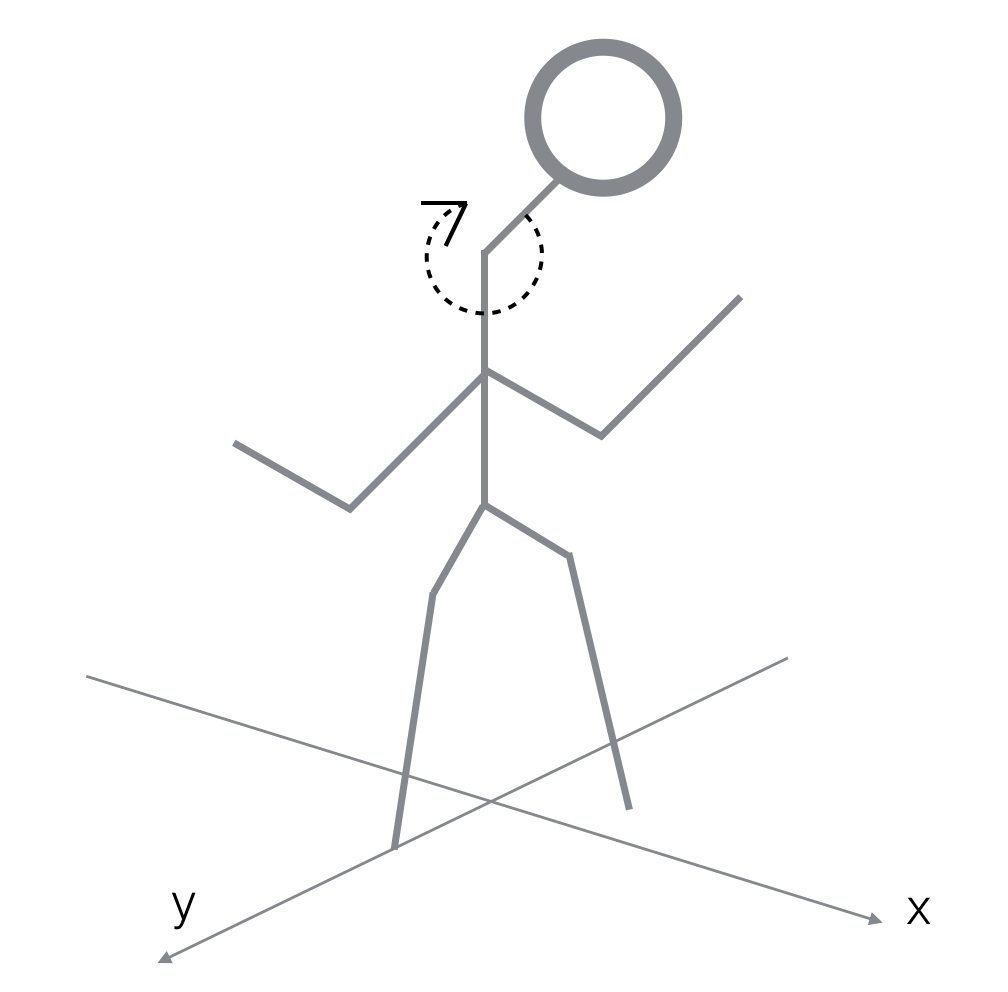
\includegraphics[width=.5\textwidth]{act}
}
\caption{躯干的平面运动与头部的转动}
\label{fig:act}
\end{figure}

但躯干的平面运动一般受场地的制约,并不是绝对的自由行进,而且由于人在看不到外界环境时处于一种对外界警惕的状态,实现行走不是全景漫游最优的运动方式。头部的转动则是一种比较好的选择,首先它的运动幅度较小,易于控制,其次头部转动也是人本能的反应,符合人对场景活动的预期。

人头部转动的形式有以下几种:低头与仰头、左歪与右歪、左转与右转。低头仰头的最大范围为 75°,另两种形式都为 110°,但低头舒适范围为 25°,仰头舒适范围为 12°。由此可得,全景漫游所用观看形式仍应以正面为主,辅以左右延展开的场景以供转头观察,这样可使人在舒适范围内使用全景漫游设备。同时,除主要场景外的功能部件也因设置在上下方向,以方便使用者通过低头仰头就可捕捉到所需要的部件。

同时,因为环境等不确定因素,易使用户丢失通过视觉等多种方式建立起的方位感。为避免方位感丢失对用户造成的迷茫,随时随地可以回到初始状态的功能也需处处设计在全景漫游中。

\subsection{手部活动}

漫游只是满足人观察的需求,需要与场景互动仍需要更多样化的操作形式。手势操作自然而然成了人控制的最佳选择,现有传感手套、指环甚至肌肉传感器可以作为全景漫游的输入装置。
  \chapter{全景漫游的交互形式}

全景漫游的交互实现有可视化界面、可配戴设备的操作以及语音指令等多种形式,本文所涉及内容主要为可视化交互这种形式,辅以其他交互形式作为参照。可视化图形化人机界面即 GUI 界面由来已久,而最早的计算机则是需要科学家通过输入带孔纸带,计算机通过读取纸带上的小孔获取输入信息来进行运算,现今计算机用户甚至连 70~80 年代常见的命令行界面都未曾见过,如图\ref{fig:gui&cli}。

\begin{figure}[htp]
\centering
\fbox{
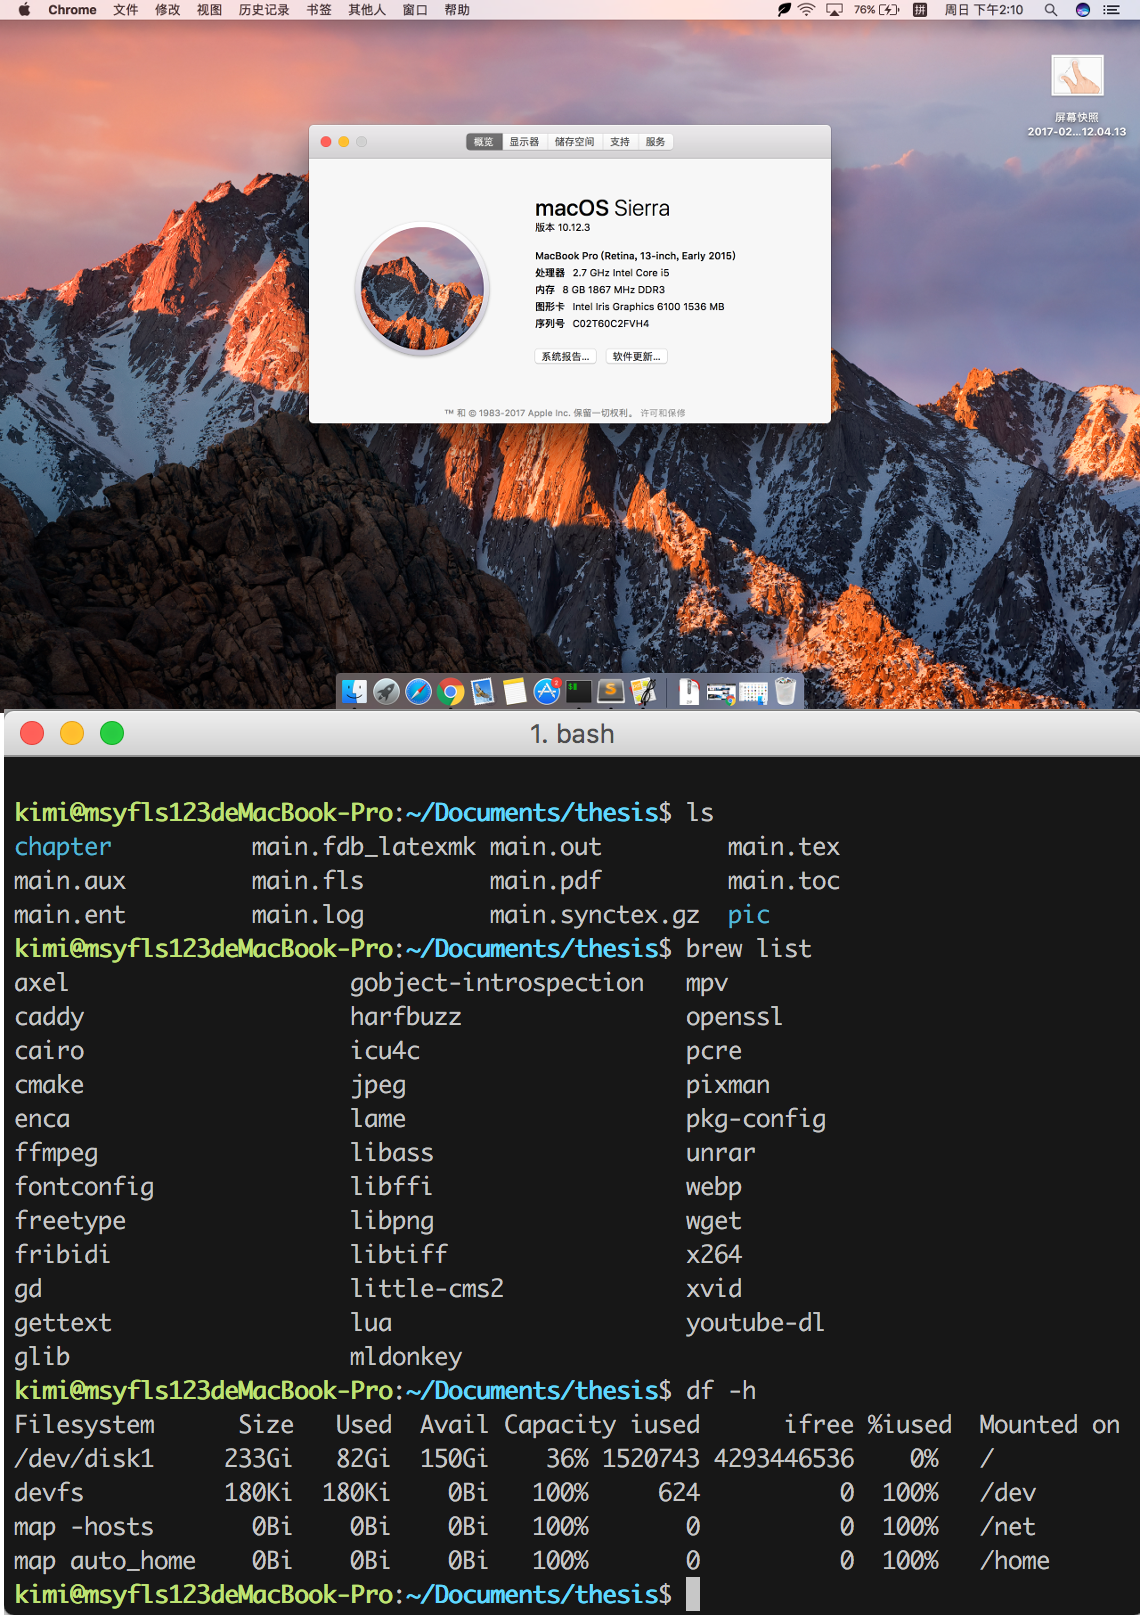
\includegraphics[width=.5\textwidth]{gui&cli}
}
\caption{图形化人机界面与命令行界面}
\label{fig:gui&cli}
\end{figure}

从命令行程序到图形化人机界面,用户获得的信息变得更多,但输入信息却减少了很多。无数复杂的程序逻辑隐藏在一次又一次的鼠标点击或是手指点按后面,用户已经不是当年那群使用纸带操作计算机的科学家了。换而言之,用户无法准确记住那么多复杂的计算机命令,更不用提理解计算机内部的程序逻辑,他们只用理解计算机可以提供给他们的功能,例如通过点击某个按钮而无须记住类似“:w”这样的程序命令即可保存文件,并善加利用即可。

而图形化人机界面毕竟信息量相比与命令行界面信息量多出好几个数量级,例如一个全屏 shell 窗口的信息量不会超过 500 字节,但是一个屏幕却有高达 $1920\times1080=2073600$ 个像素,而且图形化人机界面的信息变化效率高,可以用来表现视频动画等信息,其信息复杂度又提高了很多。

综上所述,在图形化人机界面时代随着信息爆炸而造成的信息过载(即信息的处理反馈速度低于信息生产的增长速度
,而造成信息沉积)促使信息界面的设计制作者需从信息架构的角度出发,减少冗余信息,整理信息的分布情况以使用户能更直观高效地获取使用信息。

本章将从信息架构、功能架构两条主线出发,探究全景漫游中可视化交互的可行技术路线,并结合相关理论尝试总结出部分经过实践检验或因技术选择而必然选用的功能模块,以供设计参考。


\section{全景漫游的信息架构}

全景漫游按形式可类比成游乐园,用户就像游客一样在场景中漫游,由此可以大致描绘出全景漫游的整体信息结构,如图\ref{fig:park}。这种假象的设计可以将使用者置于一种需求和环境相匹配的使用情景中,使用者可以借鉴平时游玩游乐场所积累的记忆,从场景中找寻到熟悉的“场所”以完成体验的过程。这种模式能够尽可能减少乃至消除用户对踏足陌生环境的恐惧感,人的行动预期也可以被规划在场景的设计中。

\begin{figure}[htp]
\centering
\fbox{
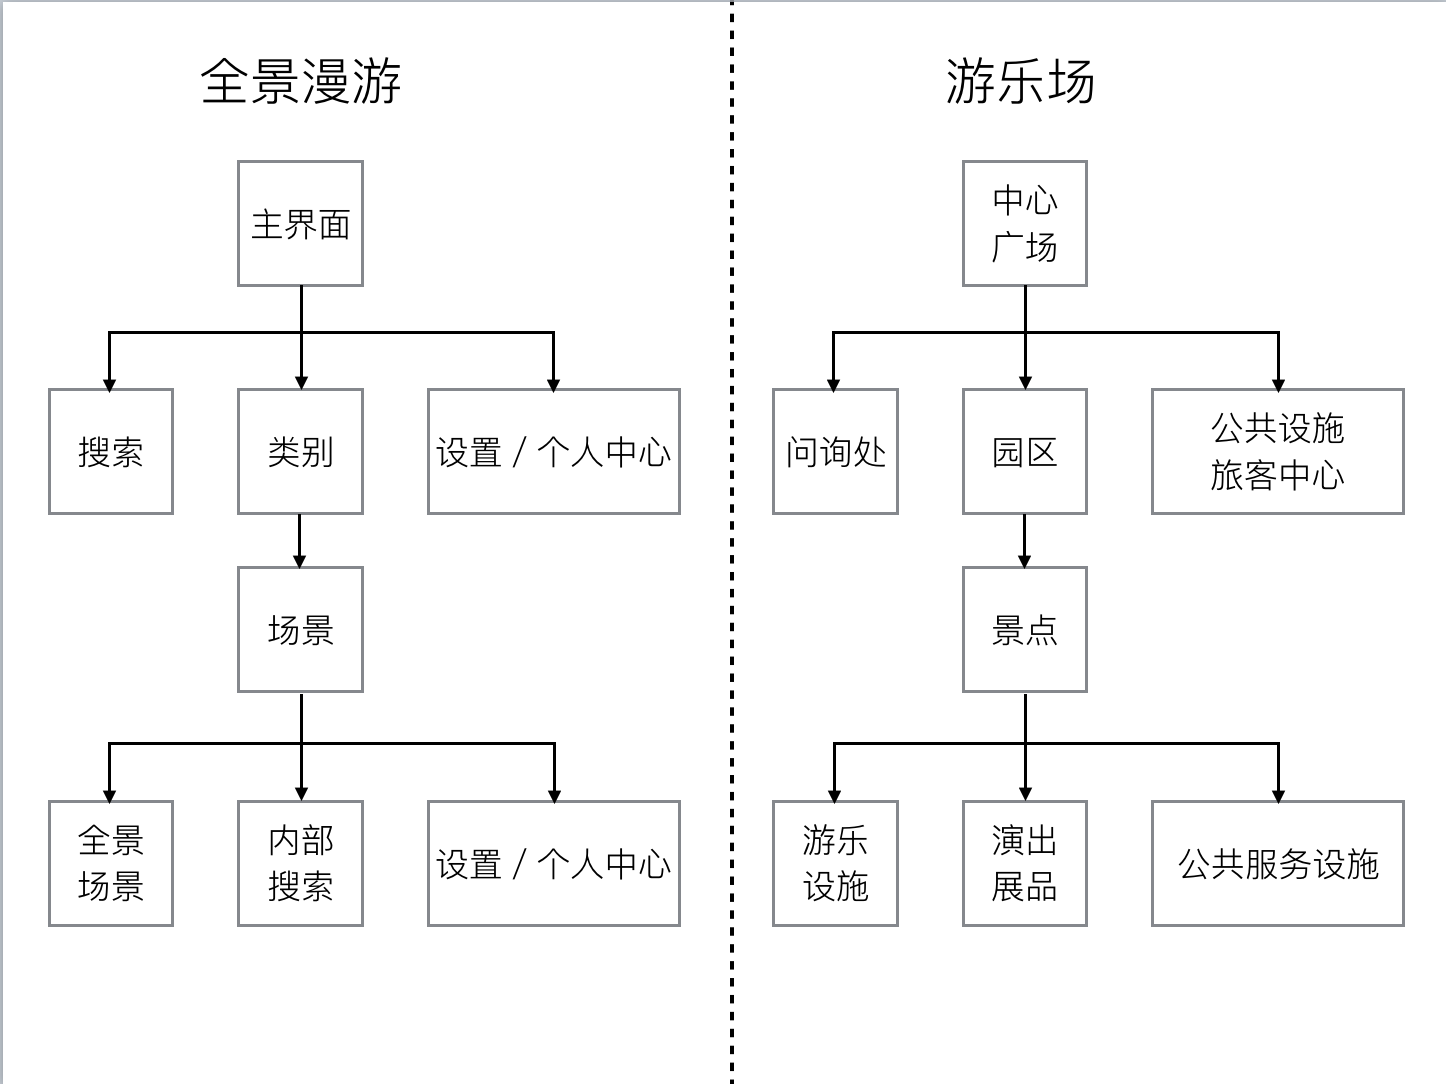
\includegraphics[width=.7\textwidth]{park}
}
\caption{全景漫游与游乐场的信息(组织)结构示意}
\label{fig:park}
\end{figure}

\subsection{信息架构组织形式}
信息架构的组织形式多样,一般而言可分为:自顶向下、自底向上和不可见的这三种形式。当前数以亿计的网站、应用和系统的信息架构都可以用它们来概括\endnote{罗森菲尔德, 莫尔维莱, 阿朗戈,等. 信息架构:超越Web设计[M]. 电子工业出版社, 2016.}。

自顶向下的信息架构是通常网页所采用的形式,其核心思想是用户已经有了一个需求概念和一个立足点(比如网站的首页),用户从首页出发,通过浏览展现的各种信息选择与自己的需求最为匹配的那个进行浏览(通常是进入下一个页面),然后在下一页面继续重复上述步骤直至找到自己所需的信息。自顶向下的信息架构非常清晰,所有类别目录都被呈现在用户面前,用户只需明确自己的需求就一定能找到“最接近”的那个页面。但缺点是层级嵌套过深时容易使用户丧失进一步浏览的冲动,而往往此时离最后的页面只差一步之遥。自顶而下的信息层级以不超过三级为宜,在全景漫游中,“主界面-类别-场景”的层级刚好是三级,所以大部分导航类的场景(页面)采用这种信息架构是可行的。

自底向上的信息架构主要应用于服务于单个目的的应用中,主要通过建立事物间的联系来帮助用户在条目间切换。维基百科就是一个很好的例子,每一个词条都有众多相关链接指向其他的百科页面,通过不同的页面联结就构成了完整的知识体系。这种联系的方式也是现代搜索引擎排序的方式,即通过互相引用的计数来判断一个信息的权重,引用计数越高说明这条信息的真实性和准确性越高。全景漫游中单个场景的设计中可应用这种自底向上信息架构,例如在某个著名景点的全景漫游中,在浏览至某壁画前时通过点击其上的热点按钮,可以弹出关于该壁画的相关信息(如图\ref{fig:dunhuang}),这种信息代入方式相比传统的图文模式更容易使人沉浸于情景中,寓教于乐的效果更为理想。

\begin{figure}[htp]
\centering
\fbox{
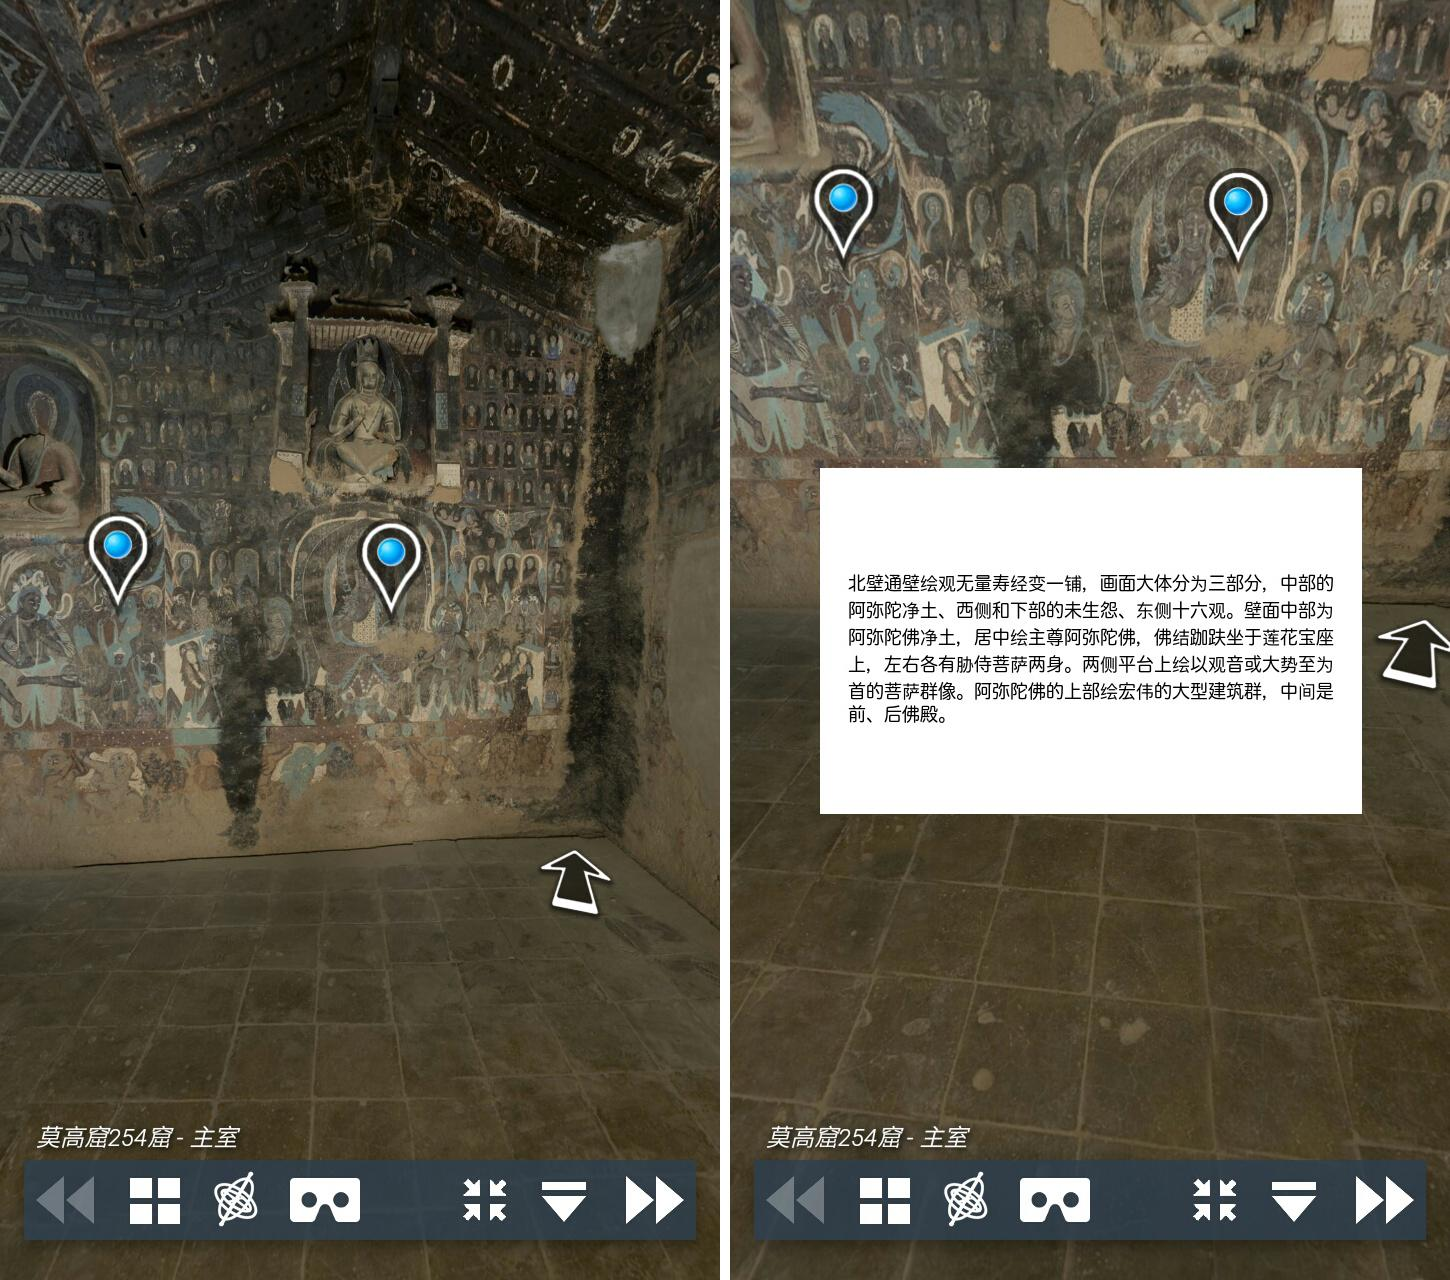
\includegraphics[width=.7\textwidth]{dunhuang}
}
\caption{全景漫游与景点介绍结合}
\label{fig:dunhuang}
\end{figure}

不可见的信息架构则包含用户输入的部分转换成特定的结构,例如用户的搜索功能等。这种信息架构有时也会影响前两者,比如通过自定义类别或提高相对信息权重来引导用户去关注某一类内容,这一点赋予了信息架构的设计管理者在设计制作完成后不断完善丰富交互内容的能力。

\subsection{信息架构组件}
信息架构的层次间可以互动,用户一般不常接触直接的层次,而是通过与信息架构组件间的交互完成信息互动。常见的组件有浏览帮手、搜索帮手、内容与任务,以及“不可见的”组件。

浏览帮手如网站的目录、导航栏、网站向导等,相当于文章的摘要和目录等,用以引导用户理解网站的大体结构。搜索帮手则是帮助带有特定目的浏览网站的用户更直接更快速地通过检索相关信息,直达自己所需信息的页面。内容和任务则是帮助带有探索目的的用户,以完成任务的形式去发现网站的功能,带有这种组件的网站一般为功能工具型网站而非展示类网站。“不可见的”组件即网站背后的算法和公式等,它们指导前台组件将用户导向更为合理高效的浏览途径上去。

在场景漫游中,内容与任务在场景内起主导作用,而在场景外则是导航与搜索起到引导用户踏足更多场景等作用。

\subsection{信息架构可视化}
信息架构不是藏在界面后面的东西,相反它出现在界面的各个角落。信息是一切操作的出发点和目的地,显然可见的信息架构有助于对此感兴趣的用户去进行深入体验。常见的信息架构的可视化体现在导航栏、搜索功能等上,但其他功能也会需要信息架构的支持,所以信息架构也被用来支持其他一切有功能的架构,以一种无形的形态在其他功能模块里实现自身的可视化。

\section{全景漫游的功能架构}
以功能目的为分类标准可讲全景漫游的功能分为:漫游功能、导航功能、搜索功能和记忆功能等。在实际应用中,功能的分块可因业务逻辑的复杂而增加或减少(如增添支付功能等)。以纯粹的体验角度而言,以上四项功能构成了用户在全景漫游中绝大部分的行为模式,故在此将它们列举出来讨论是较为合适的。

\subsection{漫游功能}
全景漫游,重在漫游。虽是全景漫游的绝对重点,但其实是设计中最不需要考虑的一点。因为对于该功能的使用,人完全是通过日常经验作出的本能反应,设计只能迎合这种需求。例如,想要让人可以观察到一个景点的全部景致就需要获取到这个地方的全景图(如图\ref{fig:hongcun}),而不是简单地提供一张平面图片去让用户想象。而要做到良好的全景漫游体验,只是提供一张全景图片是远远不够的,需要加入众多的场景互动,例如上文的点击热点展开景点的相关信息等。这部分功能可以用另一种全景体验来形容,称为“增强现实”。所谓“虚拟现实”,就是在模拟出全景场景后,再添加“增强现实”的元素,以达到以假乱真甚至超过现实一般的体验。

\begin{figure}[htp]
\centering
\fbox{
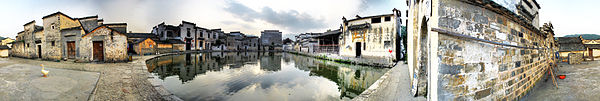
\includegraphics[width=.7\textwidth]{hongcun}
}
\caption{全景图像示例}
\label{fig:hongcun}
\end{figure}

\subsection{导航功能}
在场景间切换需要导航功能,这种导航与常见网站与手机应用内的导航基本类似,但因全景漫游的场景是空间形式的,而用户在其中并不能通过观察周围环境(虚拟场景中的地理信息通常是无效的,且脱离使用者真实所处的场景)分辨场景中的朝向,所以在场景内也通常会设置类似于一般游戏中的小地图,如图\ref{fig:minimap}。这种地图主要起到定位使用者在虚拟场景内位置的作用,原因是真实世界内使用者的位移和转向与游戏中并不完全对应,且因全景漫游体验的封闭性,人很难找到一个参考物,而地图这种形式可以方便地指明场景中角色于其他物体间的参照关系。当使用者转向时,小地图上的代表角色的图标也会随之转向,通过仔细观察并反向演算可以恢复自身的朝向感。

\begin{figure}[htp]
\centering
\fbox{
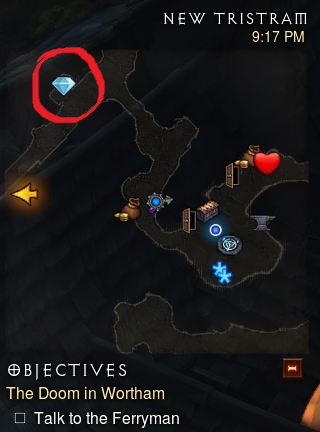
\includegraphics[width=.4\textwidth]{minimap}
}
\caption{一般游戏中的小地图}
\label{fig:minimap}
\end{figure}

\subsection{搜索功能}
搜索功能是非常常见的功能,在全景漫游中搜索功能与其他的基本类似,但因手部操作形式较为简单,故其输入文字信息的功能主要为语音识别来完成。同时,场景内的搜索功能可通过对物件的注视以获取悬浮提示的方式来选择搜索目标,即使用该物件作为搜索对象进行相关信息等检索。

\subsection{记忆功能}
记忆即储存相关信息,在探索行为中是非常重要的。记忆用户行为等目的不只是给予用户可查看的历史记录,更重要的是全景漫游中用户的操作目的性有时并不是那么明显,易造成误操作,通过还原场景功能可以撤销用户最近的若干次操作,同时可以保证场景漫游的流畅性。

系统记忆个人用户的身份信息也是有所必要的,因为每个人使用习惯与生理特性不同,系统应根据账号记忆不同账户用户的使用习惯及设置,从使用过程中自适应用户的操作,以减少用户进行复杂设置的需求。


\section{全景漫游的功能模块}
为了实现上述功能,需要在场景中插入很多组件。但组件的排序因遵循一定的规律,比如按照格式塔法则,人在注意一些相邻事物时会主动将相似的事物看作一个整体(即一个模块)进行考虑。在设计时即应按照模块化的思维对设计进行分类,模块的设计对于整个交互模式是极为重要的,好的模块设计有利于用户准确分辨并使用不同模块的功能。根据上文所述全景漫游的功能,可分为以下四个功能模块:
\begin{itemize}
	\item 导航功能模块
	\item 场景特殊模块
	\item 多输入交互模块
	\item 热点模块
\end{itemize}

\subsection{导航功能模块}
导航功能在场景漫游中使用频率并不高,主要是因为现今全景漫游大部分都只是小范围的活动,导航在整个场景漫游中起到的作用并不明显。但导航的不足会给用户带来迷茫和困惑,甚至令使用者不再愿意使用全景漫游。全景漫游力图给使用者每次带来的都是全新的历程,所以在探索新环境时,导航类的功能会给使用者提供一种情景和舒适感。

\subsubsection{导航的规则}
导航即是将东西整理并告知用户其所在位置的过程。导航的基本原则是在不影响清晰度和阅读效率的情形下展现尽可能多的信息层级结构,同时也需要指出用户当前所处的位置信息。导航除了基本的设计法则外,其规则基本遵循经验规则,如网站导航中经常采用的面包屑导航等。导航功能模块不是一个整体,通常情况下是是由一个主要的导航界面附带多个从属的局部导航功能模块所构成。优质的导航服务不会处处显露给用户其全部内容,而只是恰好在用户需要时能够在比较近的区域内找到所需的导航元素。

\subsubsection{导航的内容}
导航模块在不同场景下应该提供不同的内容。例如,主界面下就应当提供类别切换功能,而场景界面里应提供回到主屏幕的返回功能等。具体导航内容可见表\ref{tab:nav}。

\begin{table}[htbp]
\centering
\caption 界面导航内容
\vskip 5pt
\begin{tabular}{lll}
\toprule
界面 & 导航内容 & 全局导航\\
\midrule
主界面 & 类别导航、搜索功能、本地内容、历史记录 & 否\\
类别 & 类别切换、场景列表 & 有 \\
搜索 & 无 & 有 \\
本地内容 & 类别切换、内容列表 & 有 \\
历史记录 & 类别切换、记录列表 & 有 \\
单个场景 & 场景内导航(小地图等) & 有 \\
\bottomrule
\end{tabular}
\label{tab:nav}
\end{table}

\subsection{场景特殊模块}
相比于普通页面的功能模块而言,场景的特殊模块需要额外考虑自身在屏幕内的适应性。例如一个悬浮在场景内的模块,需要在与场景其他部分重叠或接触时可被分辨并识别出来。模块的设计需要考量的因素相当之多,甚至到具体实施的阶段仍会不断调整模块间的适配性。关于模块定义的具体内容会在下一章内以实例的形式进行说明,本段只对一些基本的因素作出说明。

\subsubsection{模块的单义性}
单个模块不会出现歧义,但模块一旦超过一定规模,歧义现象就不可避免地出现了,表现为重复定义模块的部分或全部。当模块间所表现出的功能相近时,用户便会产生疑惑感继而不敢做出操作或是进行重复操作。例如,最常见的是签到功能中日历当日选项和“一键签到”的按钮,其功能意义相近,但点日历也许会有查看当日信息的操作可能,所以应该无论用户点击其中任意一项都可完成签到。在设计中应当尽可能避免这种容易迷惑用户的选项,而根据不同功能设置多个单义的功能模块,这样即方便使用者识别,也降低了开发过程中的代码耦合度。

\subsubsection{模块的可组合性}
模块并不是独立存在的,模块间也会进行组合,表现为模块互相调用依赖等。比如,搜索模块也需要唤起语音输入模块来完成文本信息的录入,否则就失去了搜索的能力。同时,模块有时也会如队列般排列,比如重要操作都会需要二次验证,最简单的形式就是弹出一个确认框模块,只有用户选择了“确认”后才会继续完成后面的流程。


\subsection{多输入交互模块}
主要表现为语音输入模块、重力感应模块等。用户通过多种方式进行输入,设计时需要考量模块总输入的过滤筛选,并加以整合进行输出。

值得注意的是,全景漫游功能是建立在重力感应的技术基础上的,故最贴近其使用形式的交互模式可以采用摆动头部这类动作的形式。可以通过实验方式采集每种基础头部动作的三维运动加速度,经过预处理后作为头部动作的特征量,然后通过建立隐马尔可夫模型后对实际运用过程中采集的头部动作数据进行识别,转化为基础头部动作的序列,达到头部动作实现交互操作的功能\endnote{孔俊其. 基于三维加速度传感器的手势识别及交互模型研究[D].苏州大学,2009.}。

\subsection{热点模块}
场景中有很多非通用但也具有交互能力的模块,统一将其设计称为一个触发器,当用户选择后便给它发出一个激活信号,令其执行预定的操作。热点模块类似于生活中电器的开关,随处可见非常普通但也很重要。

  \chapter{全景漫游的交互模型}
全景漫游中的用户交互属于典型的多通道交互,根据前文所列举的关于人的意识的相关理论可知,人在面对多通道输入的刺激时,会或主动或被动地选择一种进行注意。如果这些刺激可以达到被人记忆并在需要时主动唤起的效果,那有可能在多通道输入中自动加工处理,减少对人的脑力资源的占用。同时,经过良好规划的交互模型也能避免用户出错的概率,提高网络资源的利用率,降低后台服务器程序处理的负担。

基于上述假设,尝试通过认知理论对全景漫游中设备端交互、菜单交互和场景交互,分别构建交互模型。以期通过多种形式展现信息,达到更高效表达场景的意图,结合人与设备的关系切实提升用户操作体验。

\section{设备交互}
交互从人发出的信息至被设备捕获转换为数字信号是一个明显的“编码/解码”的过程。人的动作相当于人通过分析相关信息,并试图理解机器的运作模式,认识到自己所需表达的信息,最后发出了一个按照“所认为机器能够理解的方式”进行编码的“信号”。而设备则是处在各种信息的海洋中,一刻不歇地从外界收集信息,当成功捕获到一个匹配其预设规律的“信号”时,通过确定的解码方式,还原出人最初想表达的信息。

\subsection{信息流与反馈等待}
设备无时无刻不在等待着用户的信息输入,而用户的输入是多通道的,在不同的通道上都会捕获到用户的输入流。多输入流经过处理后在主信息流上合并成一条输入流,由设备程序进行集中处理。如图\ref{fig:reactive}。

\begin{figure}[htp]
\centering
\fbox{
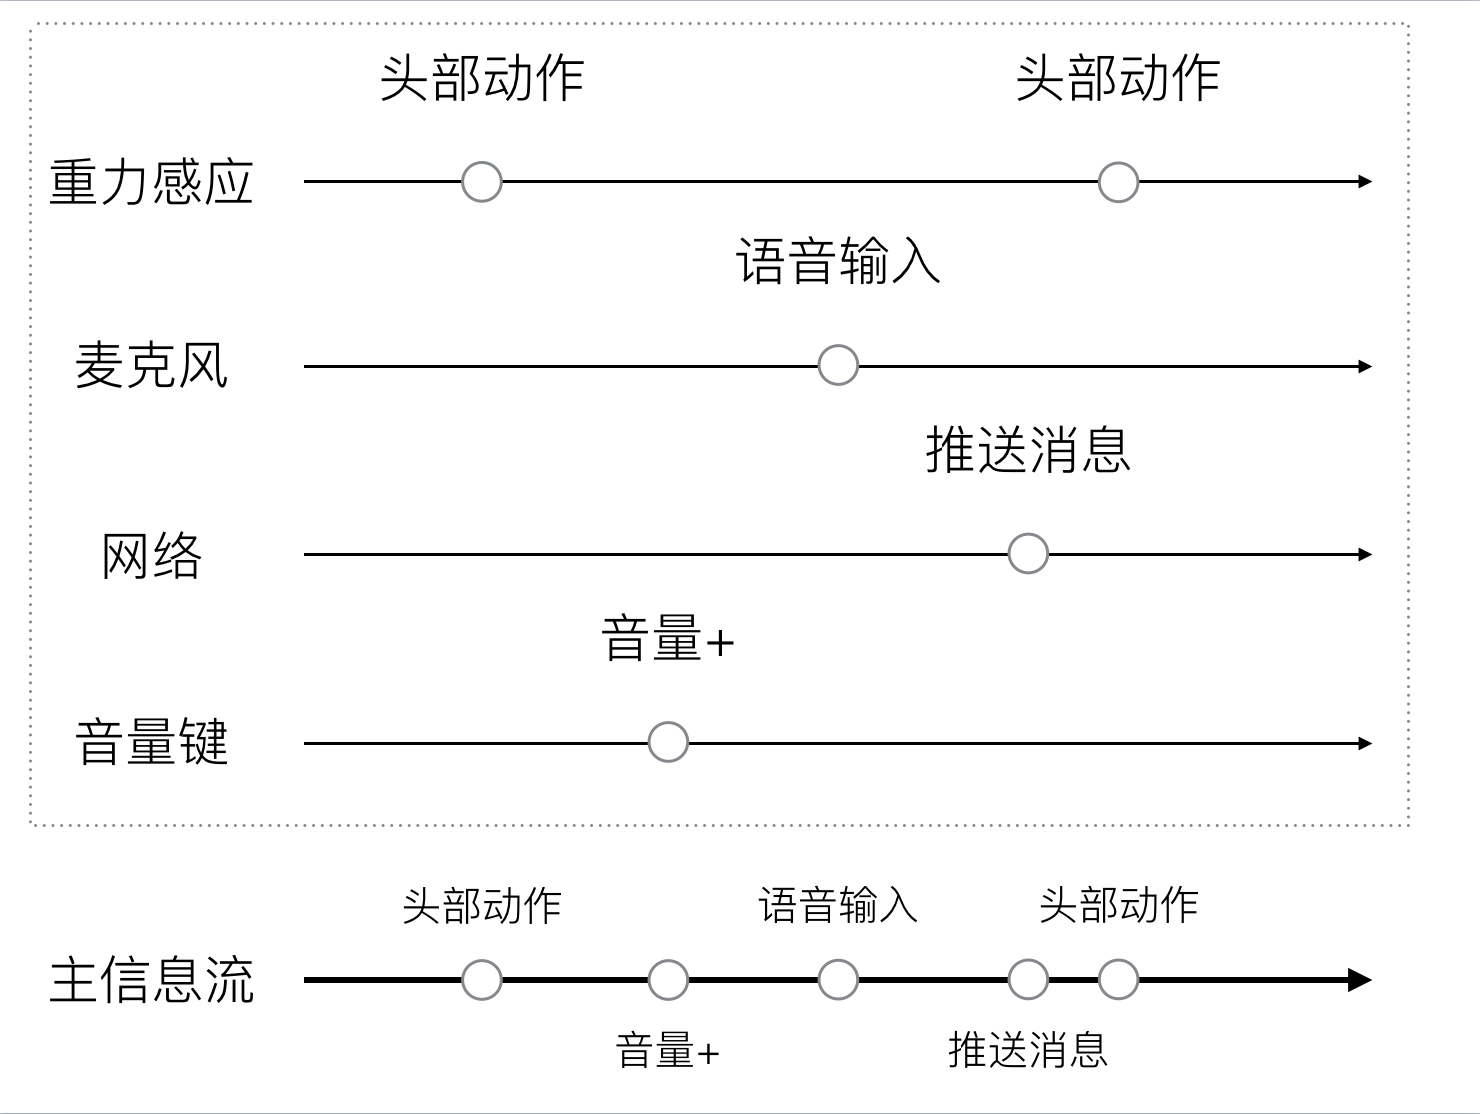
\includegraphics[width=.5\textwidth]{reactive}
}
\caption{信息流}
\label{fig:reactive}
\end{figure}

但常见的场景是,交互行为的发生与处理完成得到反馈并不是即时的,而要经过一定的时间,其等待时间因网络延迟或设备响应而不一。这时用户等待的过程就会形成一阵交互效果上的“盲区”,也就是常见的“设备无响应”状态,如图\ref{fig:stream}	。“设备无响应”情形在一般设备上出现并不会造成过大的后果,但是在全景漫游中用户的视野处在封闭的空间中,长时间得不到合理反馈易造成用户心理恐慌,是需要通过设计极力避免的情形。

\begin{figure}[htp]
\centering
\fbox{
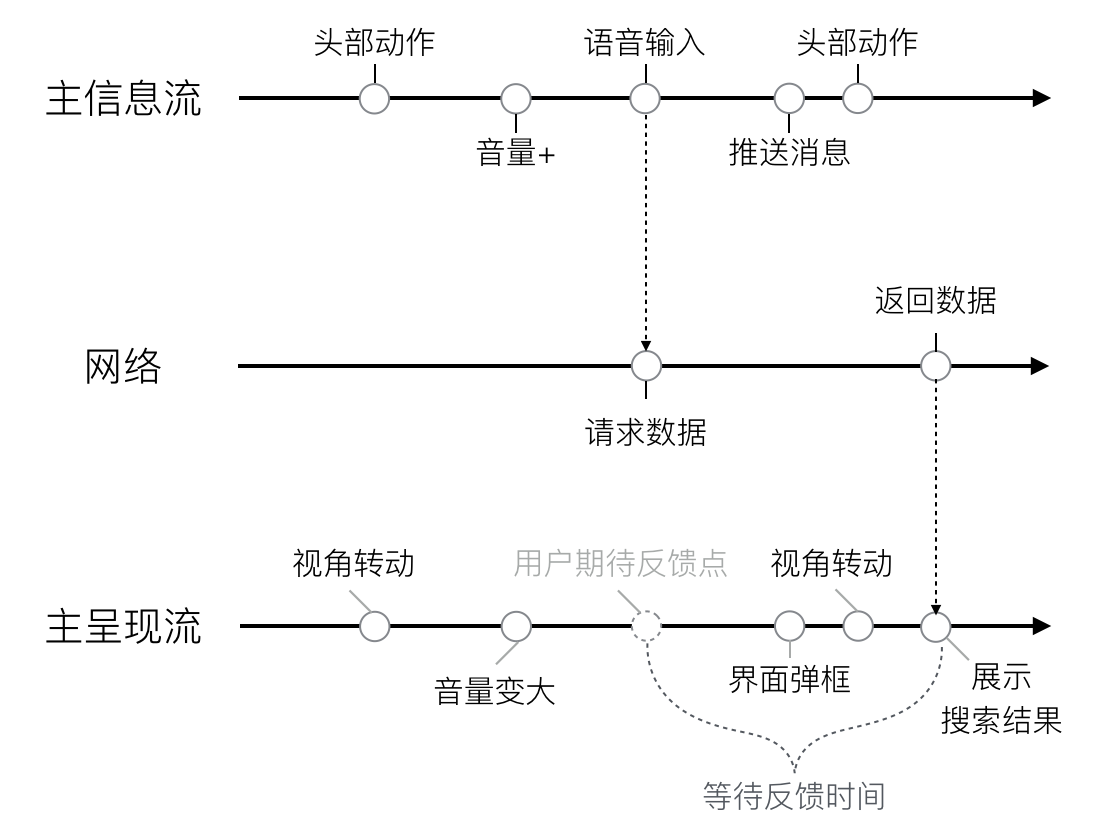
\includegraphics[width=.5\textwidth]{stream}
}
\caption{交互中因其他元素造成的等待}
\label{fig:stream}
\end{figure}

即时反馈信息是最理想的方案,但现实情况必须对此作出解释以避免用户等待无反馈而产生迷茫情绪。常见的方案是对用户的输入做出即时反馈,当反馈不能即时给到时给出等待反馈的提示。前文所提到的通过注视(gaze)一定时间而做出确定选择的过程就是一种非即时的操作,在等待确认完成过程中通过一些标示告知用户:此处正在等待完成的行为是什么,预计完成的时间是多少等。

\subsection{信息修正}
信息流的出现帮助解决了信息加工过程中信息传达时间不一致的问题,但用户有可能得到的信息不准确或是很模糊,需要用户去判断信息是否符合预期,在无法判断信息的有效性时,如果能够提供给用户一个可以自我纠正的语境,将有利于用户自己辨别信息\endnote{路璐,田丰,戴国忠,王宏安. 融合触、听、视觉的多通道认知和交互模型[J]. 计算机辅助设计与图形学学报,2014,(04):654-661.}。

例如,在导航过程中提供给给用户当前朝向与正确方向的箭头图示,用户会尝试向左或向右转向,当向左转时会发现偏离变大,而向右转时会发现偏离变小,用户自然会选择向右转以回到正确方向上去,如图\ref{fig:correct}。

\begin{figure}[htp]
\centering
\fbox{
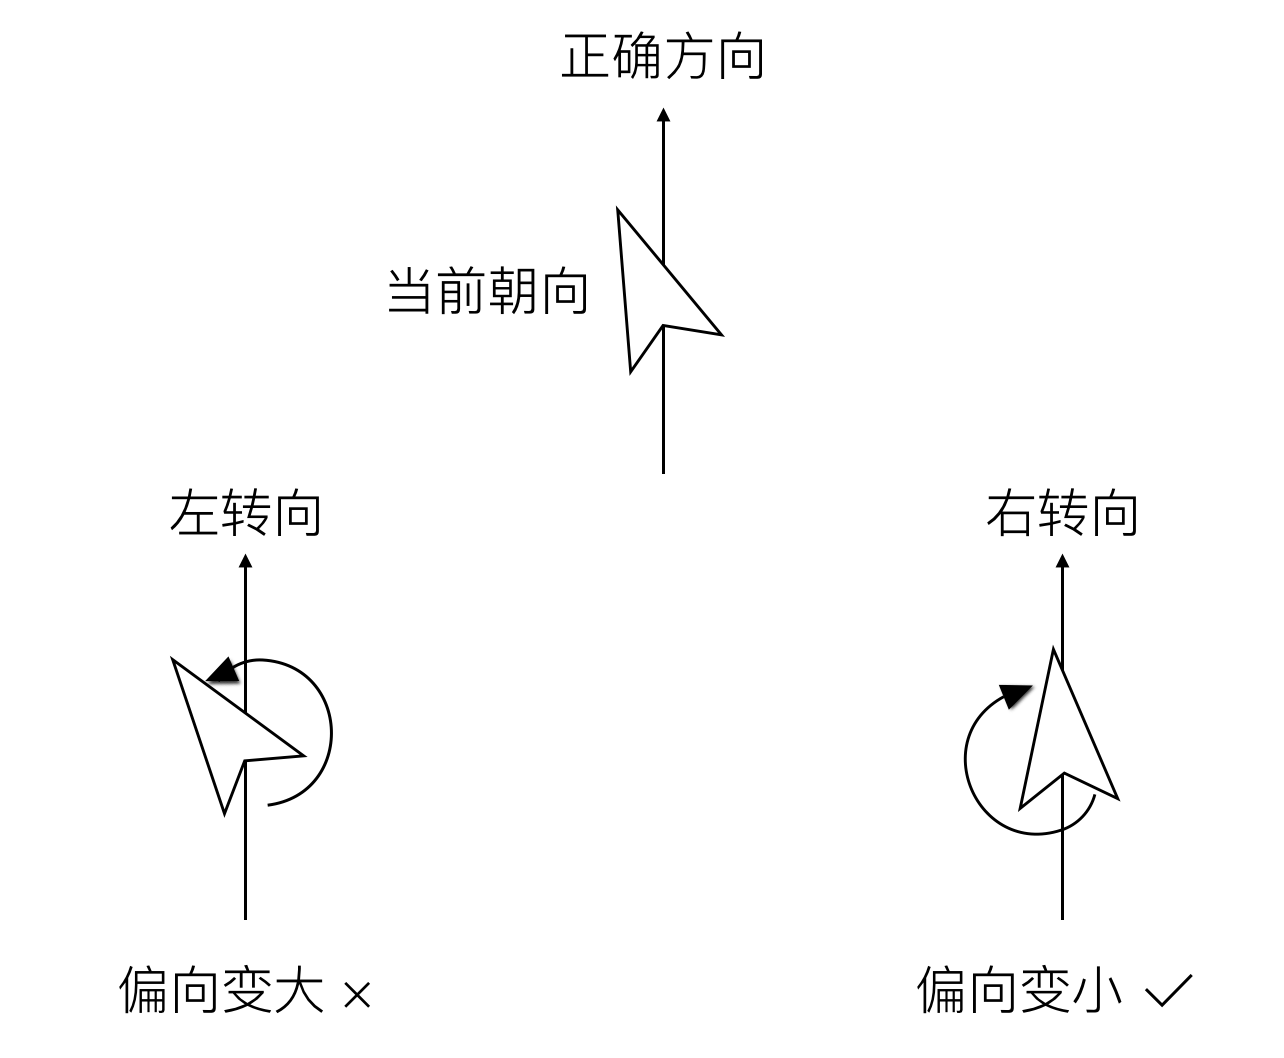
\includegraphics[width=.5\textwidth]{correct}
}
\caption{自我修正的交互行为}
\label{fig:correct}
\end{figure}

在全景漫游中与设备进行多通道交互是可行且必要的,人的感官可以从不同通道间获取信息,使人获得的信息更为全面。更为关键的是多通道信息往往能够起到互补的作用,使得信息交互的鲁棒性大大提高,也使用户对于系统和环境的适应性得到了提升。而全景漫游因与普通的设备交互有所不同,故应加强信息流的建立,避免用户无谓的等待,提高交互的流畅性。而在交互的结果上注重信息的可修正性,帮助用户通过自我反馈建立准确有效的信息流。

\section{导航交互}
全景漫游中导航功能的重要性不言而喻,但场景中元素的可识别要求又限制了导航功能的复杂度。导航应符合用户对信息整合的需求,而又对场景内容起烘托作用。由前一章信息架构的组织形式可知,导航应包括自顶向下、自底向上、不可见联结这三种基本信息组织形式,它们分别体现为导航层级的上下文感知、单个内容增强信息展示和多任务切换。

\subsection{上下文感知}
上下文是指当前环境中区别于当前本体的因素。上下文按与用户关系可简单分为主动上下文和被动上下文两种。主动上下文指环境中可以直接改变系统行为的状态或变量。被动上下文指那些虽不能直接产生作用但可引起用户兴趣继而通过用户改变系统行为的状态或变量\endnote{张磊. 上下文感知在导游系统中的应用[A]. 中国计算机学会、中国图象图形学学会、ACM SIGCHI中国分会、清华大学计算机科学与技术系.第一届建立和谐人机环境联合学术会议(HHME2005)论文集[C].中国计算机学会、中国图象图形学学会、ACM SIGCHI中国分会、清华大学计算机科学与技术系:,2005:4.}。上下文感知是指计算实体能够根据上下文环境的变化及时调整自身行为,使用户从信息的管理和输入中解放出来,专注于要执行任务的本身\endnote{王守芳, 金浩, 魏鲲,等. 上下文感知综述[C]// 建立和谐人机环境联合学术会议. 2005.}。

上下文感知的作用非常重要,没有上下文用户很难预计进行操作时即将发生的变化,容易在使用过程产生困惑。网页等在通过列表批量展示内容时都会同时展示该内容的多项信息,包括名称、录入时间、信息量等(可能因内容类型不同而信息名称有所差异)。例如商城类网页会展示商品的名称、产地、出厂时间等,这些信息就是上下文。通过阅读理解相关信息,用户可以在不打开具体页面的情况下对相应项目得到一个基本的认识。

上下文感知发生在上下文环境的改变过程中,具体表现为上下文语境的重构,即移除不再相关的组件,添加新的相关组件,同时改变组件间的联系等\endnote{李玲玲,高新. 基于上下文感知的移动计算应用[J]. 软件导刊,2011,(06):17-18.
}。

例如,在前文所提出的列表展示内容的页面中,当用户切换列表界面时,界面上标签的语义发生了变化,如图\ref{fig:context}。图中上半部分为分类的菜单,下半部分为某一分类的更多页面。上半部分中三个标签分别是不同的分类,而下半部分的三个标签则是针对同意分类的三种不同筛选方式。虽然两者形式上类似,但标签的语义截然不同。

\begin{figure}[htp]
\centering
\fbox{
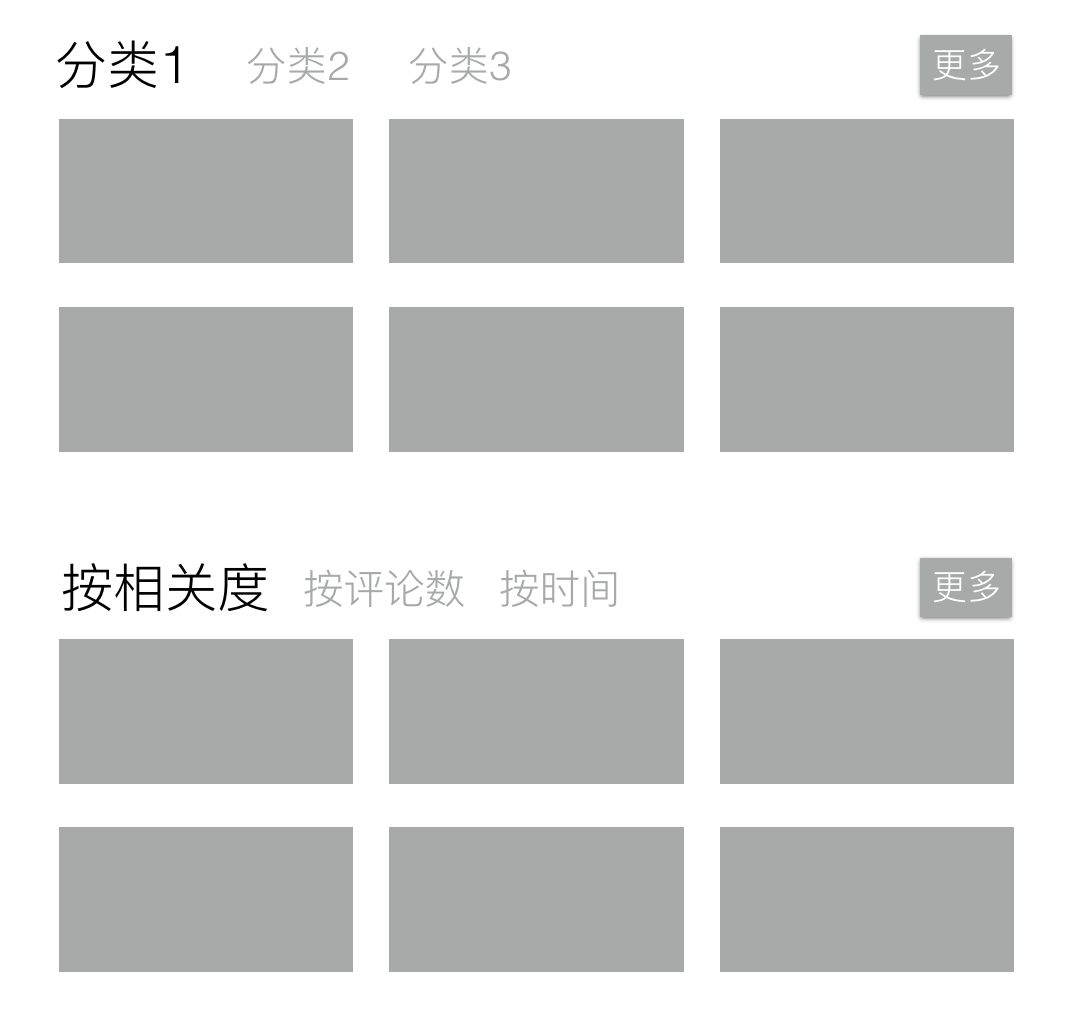
\includegraphics[width=.5\textwidth]{context}
}
\caption{上下文语境的重构}
\label{fig:context}
\end{figure}

\begin{table}[htbp]
\centering
\caption{分类菜单和单个类别菜单的语义}
\vskip 5pt
\begin{tabular}{lll}
\toprule
栏目 & 分类菜单 & 单个类别菜单 \\
\midrule
数据集合 & 不同 & 相同 \\
切换方式  & 点击标签 & 点击标签 \\
标签意义 & 集合代称 & 筛选依据 \\
\bottomrule
\end{tabular}
\label{tab:collection}
\end{table}

在上下文语境的重构过程中,语义的变化如表\ref{tab:collection}。表中可知,用户在语境切换后操作方式没有变化,依旧为点击标签,但单个标签的意义和数据的集合都发生了改变。这种情况下就容易造成上下文环境的语义混淆,需要直观且清晰地提示用户场景的语境已经发生变化,并标注上可供用户理解当前上下文环境的关键信息(如当前栏目的标示等)。

如图\ref{fig:tab},在 PC 端网页中,常用的标注语境的方式是一种“面包屑导航”,将从首页至当前页面所有途径的页面名称罗列出来。而在移动端设备上,因屏幕宽度上有限制,常用的做法是在顶部功能栏正中标注出当前栏目名称。而在全景漫游中,因界面不一定限制于二维空间内,故可以采用按深度排列的界面,以标示用户途径的界面。用户在切换界面时,同时可以看到曾经访问过的页面的一部分,容易理解该页面是由前一个页面中的部分扩展而来,对整体信息架构也会产生一定的了解。

\begin{figure}[htp]
\centering
\fbox{
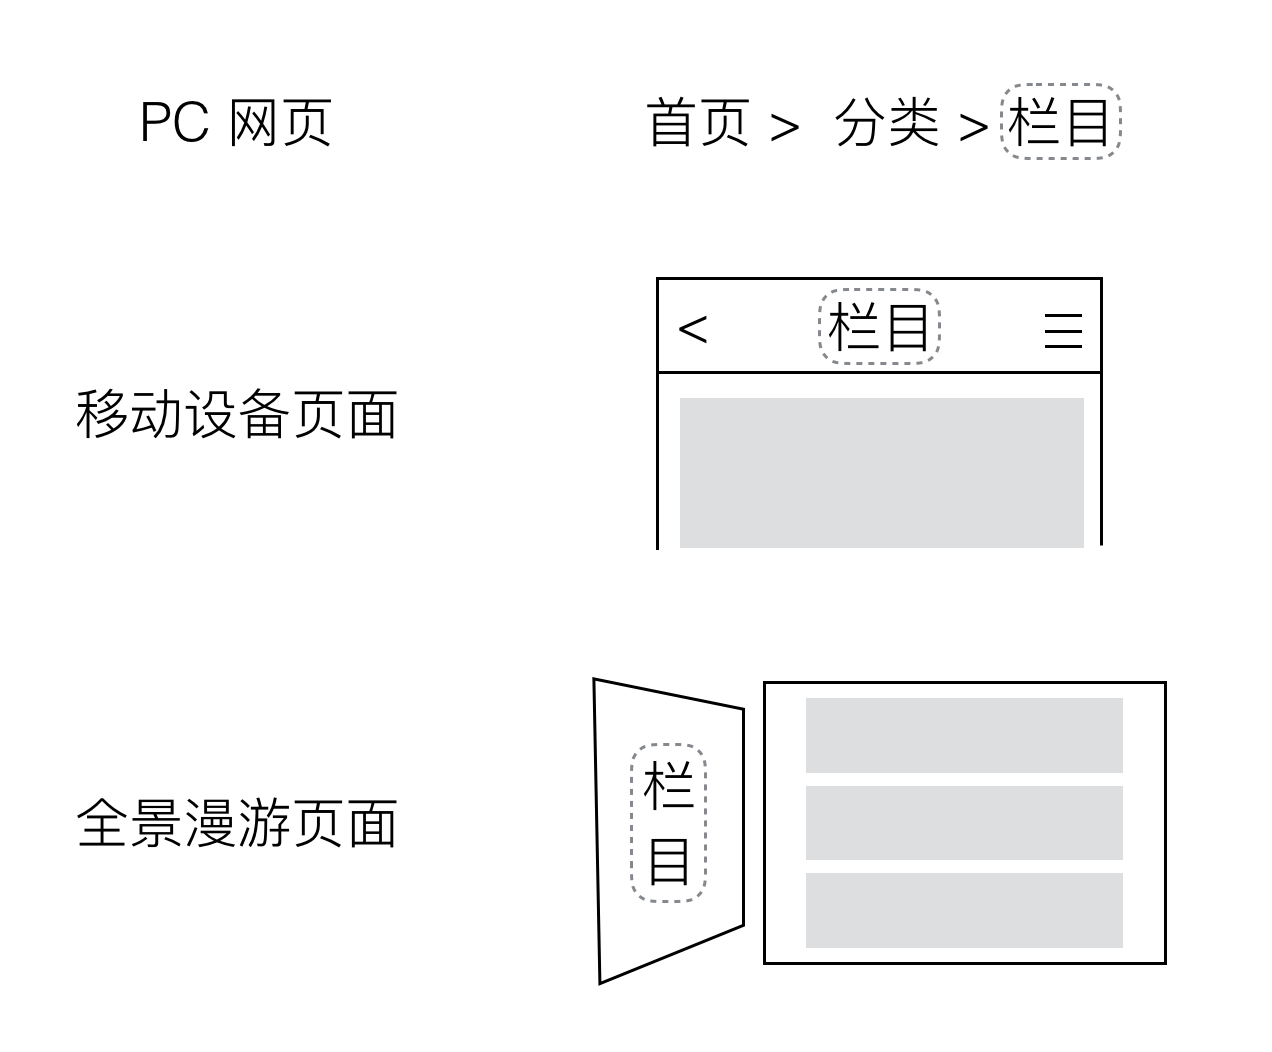
\includegraphics[width=.5\textwidth]{tab}
}
\caption{不同设备状态下的页面语境标示}
\label{fig:tab}
\end{figure}

在全景漫游的界面设计中,应当尤其注意语境的建立,以帮助用户更清晰地认知自身在导航功能中的位置,同时建立起对上下文环境的基本感知。

\subsection{增强信息}
在单个页面里尽可能多地铺陈相关信息,包括其他相关内容,减少用户反复查找的负担。信息的增加看似会对用户造成认知上的负担,但经过良好组织的信息是容易被用户快速接受的。增强信息的本质是还原给用户真实且有效的足量信息,但信息的形式应易于用户识别。研究显示,在理解复杂概念时,人对图像(尤其是图形)信息的理解准确度和速度相比理解文本信息均有一定程度的提高。而对同为文本信息的内容而言,人对数字这类表义性单一的文字识别能力也高于对其他语言的识别。故可以假设信息易识别性公式 \ref{eq:recognize}。

\begin{equation}
Icon > Graph > Number > Character 
\label{eq:recognize}
\end{equation}

根据上述内容可知,增强信息的重点在于加强图像或数字类信息的应用。结合当前设计潮流,图像和数字的确是现代网络环境下界面设计的主要构成元素,故将其作为信息的增强和补充说明是合理的。例如,在世界自然基金会(WWF)推出的 WWF Togother 主题应用中,在展示各种动植物的项目时,以数字形式展现动植物的年均生育率、平均身高、体重,以在地球模型上标示的不同颜色区域展现动物的栖息地,甚至通过 GPS 系统向用户展示当前于该动物栖息地间的距离,使用户对该类动植物的生态状况有直观的了解。这种展示方式既能充分地向用户展示相关信息,而且可以将用户代入到场景中,引起用户感同身受的心理,加强生态保护教育的记忆。

\begin{figure}[htp]
\centering
\fbox{
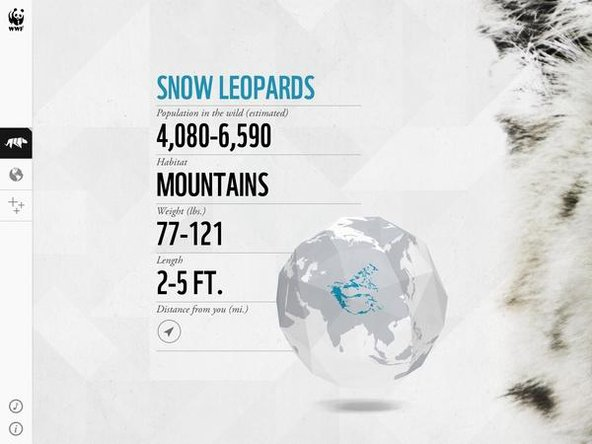
\includegraphics[width=.5\textwidth]{wwf}
}
\caption{WWF Together 主题应用截图}
\label{fig:wwf}
\end{figure}

将增强信息置于上下文语境内考量时,其应用符合人的心智模型对于信息架构的认知。从宏观角度看,用户进入应用场景时的心智模型于设计者设想的心智模型是有所冲突的,理想的应用场景应是用户一进入应用就能立即发现感兴趣的项目,但受限于现有技术能力和信息隐私的限制,用户进入场景时的心智模型是比较不符合预期的,但随着使用认知的改变而发生变化。通过信息增强令用户获得足够的有效信息,在客观上也就是使交互界面与用户的使用习惯和 生活认知相契合,最终使用户心智模型与交互模型达到匹配\endnote{林一,陈靖,刘越,王涌天. 基于心智模型的虚拟现实与增强现实混合式移动导览系统的用户体验设计[J]. 计算机学报,2015,(02):408-422.}。

\subsection{多任务切换}
在当下计算设备的计算能力飞速提升的今天,支持多进程已是一个操作系统必备的能力,用户往往会在社交应用和工具应用中来回切换,切换任务的过程存在消耗,而这其中往往消耗掉的是用户对于当前任务状态的认知。多任务切换时保留被切换应用的状态可以帮助用户留住关于该任务的部分认知,而当用户需要切换回该任务时可以通过留存的任务状态快速回到之前工作的状态。展示多任务切换的方式有很多中,相比而言最为直观的是类似 Mac OSX 的任务窗口收缩进 Docker 栏的方式。借鉴其多任务的切换方式,可以设计全景漫游中不同场景间切换的实现方式,如图\ref{fig:multitask}所示。

\begin{figure}[htp]
\centering
\fbox{
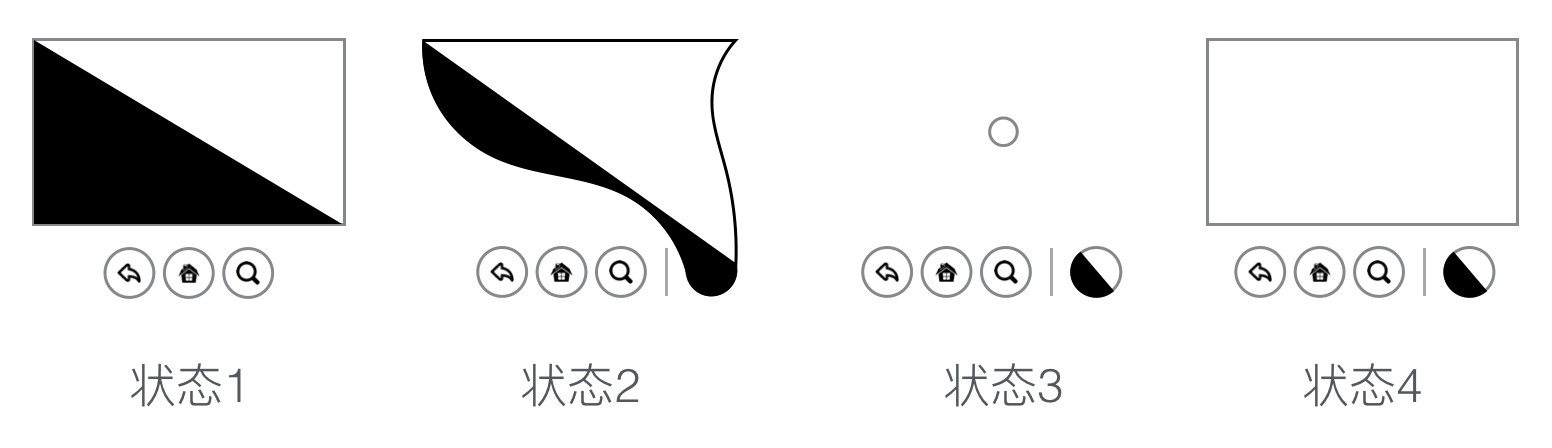
\includegraphics[width=.7\textwidth]{multitask}
}
\caption{多任务切换的交互场景}
\label{fig:multitask}
\end{figure}

上图分为四个状态
\begin{description}
	\item [状态 1] 正在使用应用 A
	\item [状态 2]用户主动打断应用运行或是用户收到系统信息而转去应用 B,此时应用 A 以 一种类似布绢收拢的形式缩小至底部全局导航栏的一侧
	\item [状态 3] 应用 A 已完全最小化到导航栏内,同时应用 B 以一个小圆点进行扩展的形式开始打开
	\item [状态 4] 应用 B 完全打开
\end{description}

此时用户能够明确地认识到应用 A 并未被关闭,同时可以通过导航栏中应用 A 的图标再次进入应用 A 并回到先前工作状态。这样就实现了用户心理上对于任务进程的闭环认识,避免用户因无法返回先前的使用状态而从头开始操作的问题。同时多任务也符合用户对于全景漫游场景应用的期望,即在一个应用中完成多种不同类型的任务,有助于提高用户的期望确认度。已有研究表明,用户的期望确认度对满意度和持续使用意愿均有显著的正向影响\endnote{代宝,刘业政. 基于期望确认模型、社会临场感和心流体验的微信用户持续使用意愿研究[J]. 现代情报,2015,(03):19-23.},故多任务切换的功能对全景漫游应用的体验起到了提升的作用。

综上所述,在进行全景漫游的导航系统交互模型设计时,因考虑不同路径不同结果取向的导航形式,并结合全景漫游在空间上的延展性,充分利用周边资源建立用户可认知的信息架构。在宏观层面上,注重上下文语境的建立,以方便用户辨别当前所处位置,在微观层面上,注重语境的内部转换和外部转换场景,使用户对于应用的整体认知保持统一(见图\ref{fig:env})。

\begin{figure}[htp]
\centering
\fbox{
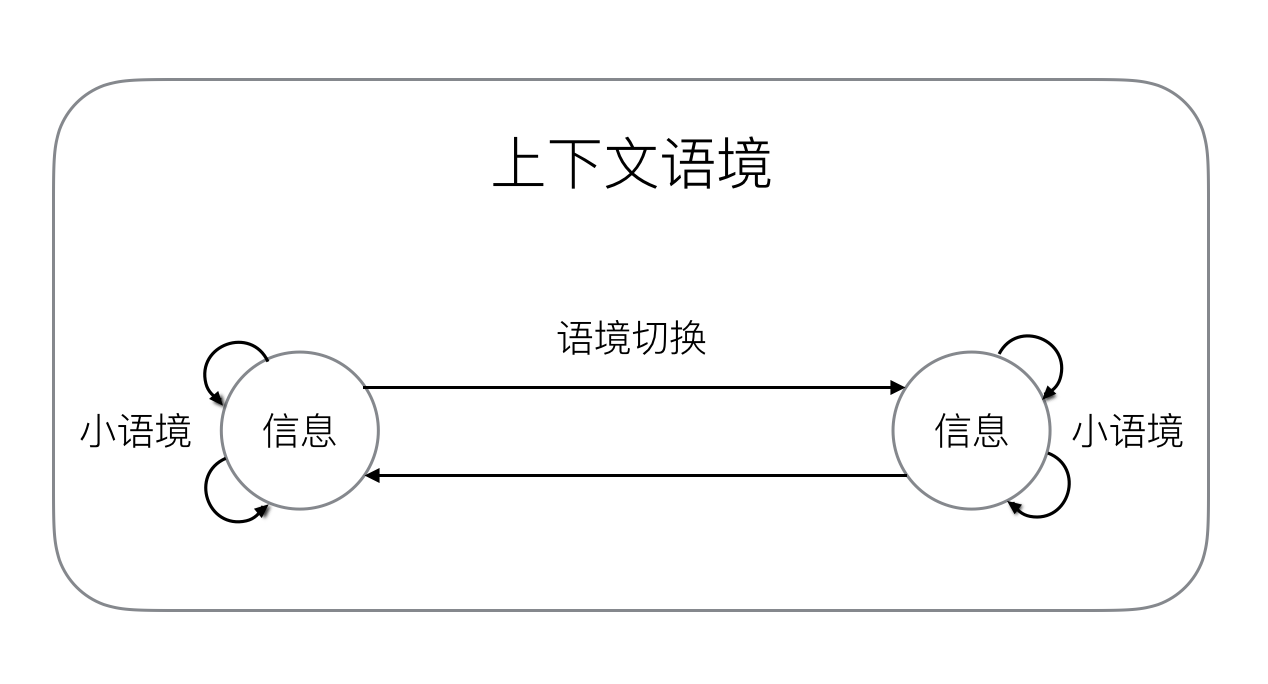
\includegraphics[width=.7\textwidth]{env}
}
\caption{全景漫游的语境建立}
\label{fig:env}
\end{figure}

\section{场景交互}

场景交互是全景漫游的核心功能,其他所有功能都是为了满足这个功能而实现的辅助内容,场景交互的质量直接关系到用户对于应用的满意度和持续使用意愿等心理性质。场景交互的主要对象是场景内的路径、全景图、可交互物件等,它们都是以一定形式储存的三维坐标信息。故研究场景交互时,从数据角度切入交互的实现过程是可行且必要的。

\subsection{场景漫游路径}
场景交互的形式如果按照漫游路径是否可由用户自主选择的角度,可分为定点路径、定向路径和非定向路径等三种。

从全景图片角度考量,定点路径是指用户仅可在按固定的若干点观察全景视图,定向路径是指用户可在一条固定的路径上观察,而非定向路径则是指用户可在任意点观察全景视图。显然,人眼直接观察景物的方式是非定向路径的形式,但以当前的技术水平和成本考虑这是不太容易实现的。定向路径就是通过预先设置漫游路径,然后再播放漫游路径的方式来实现在三维场景中的受限漫游,这种技术当前在实现上是较为成熟的\endnote{尚建嘎,刘修国,郑坤. 三维场景交互漫游的研究与实现[J]. 计算机工程,2003,(02):61-62+251.},其数据形式本质上就是全景视频。定点路径则简单得多,只是按定点序列采集的全景照片。这三种漫游路径,其成因如图\ref{fig:visual}。

\begin{figure}[htp]
\centering
\fbox{
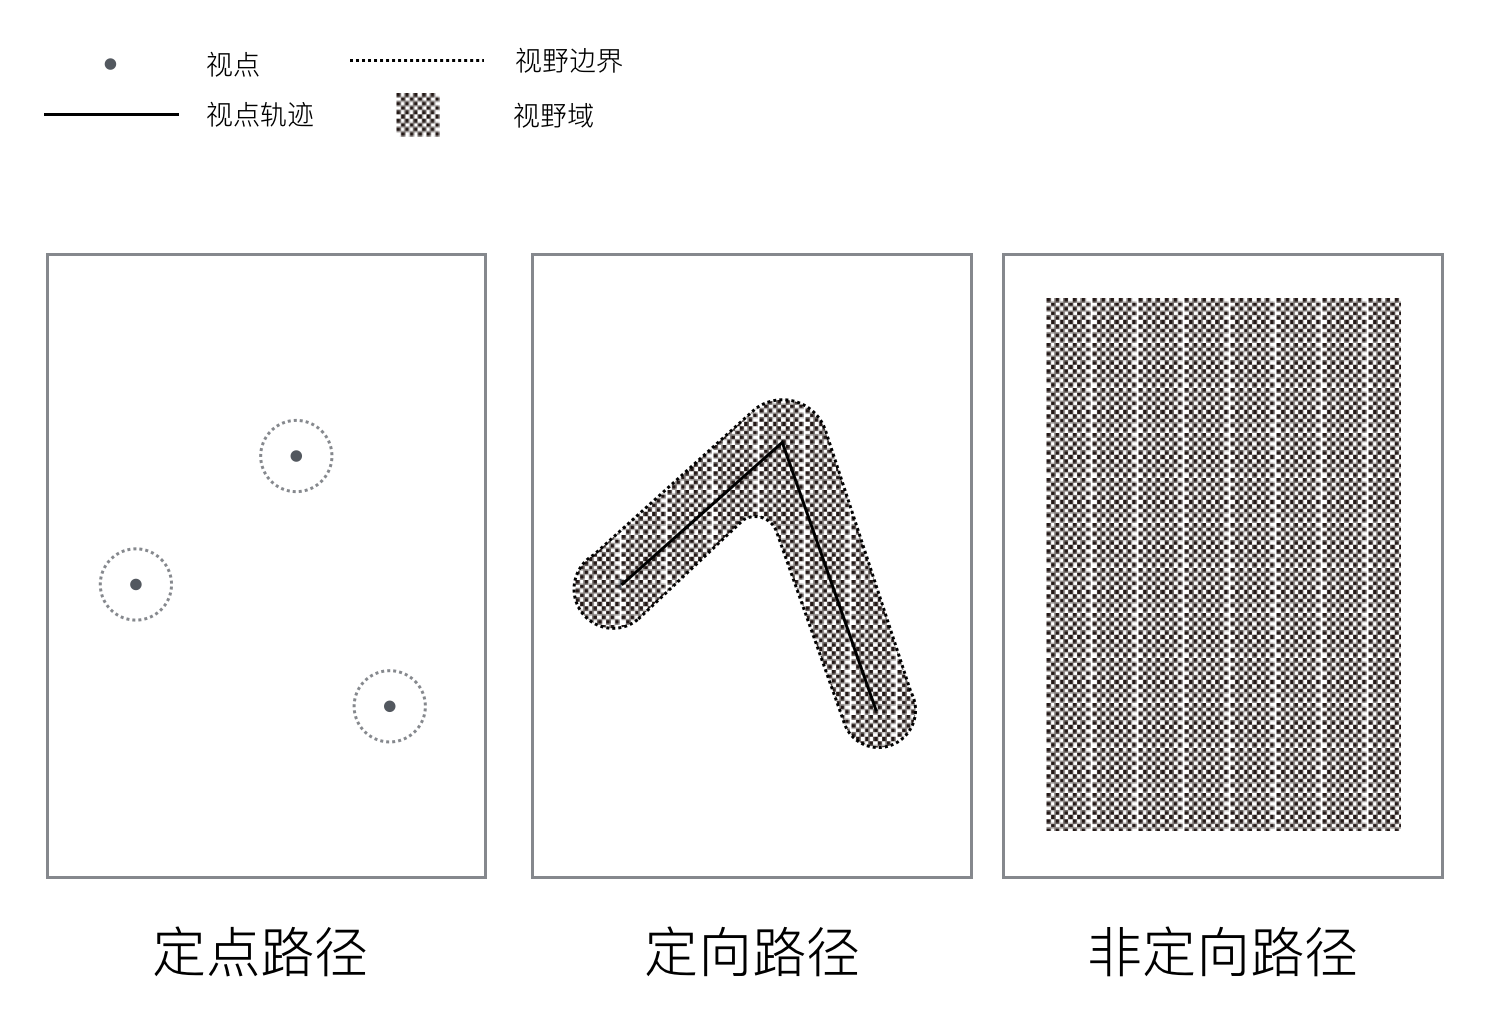
\includegraphics[width=.7\textwidth]{visual}
}
\caption{全景场景的漫游路径}
\label{fig:visual}
\end{figure}

故全景漫游的不同应用情景中,以成本角度考虑,最经济的做法是作定点路径,就是拍摄数张全景图,通过程序构建可供漫游的场景。在重要应用场合,路径较为简单(如直线行进)的情况下,可以考虑通过全景摄像机拍摄一段路径上的照片,采用定向路径漫游的形式。但可以预计到的是,从全景图片升级到全景视频,其复杂程度由会呈现巨量增长。经作者估算,一般全景漫游路径选择对全景数据空间复杂度的关系如表\ref{tab:complex}。

\begin{table}[htbp]
\centering
\caption{全景漫游路径选择数据空间复杂度\newline(以单一全景图作为 1 个单位)}
\vskip 5pt
\begin{tabular}{lll}
\toprule
路径 & 全景图 & 全景视频 \\
\midrule
定点路径 & 1 & t \\
定向路径  & n & $nt$ \\
非定向路径 & $n^3$ & $n^3t$ \\
\bottomrule
\multicolumn{3}{l}{\small 注:t 为单位时间,n 为单位路径}
\end{tabular}
\label{tab:complex}
\end{table}

其中,除了定点路径全景图和全景视频以及定向路径的全景图以外,其他三种漫游路径形式在当前技术都是难以实现的。从图片的组织形式上看,定点路径的全景视频和定向路径的全景图并没有区别,都是一系列的图像帧。从长远角度看,全景漫游的形式会趋向以全景视频或定向路径形式的漫游为主的漫游形式,但如采用定向路径的漫游形式可能因真实场地限制而无法获得理想的漫游体验。故当下仍以离散的定点路径全景图像为主,场景间的切换逻辑是全景漫游交互设计过程中重要的部分。

\subsection{场景切换标识}
场景切换过程中指示场景信息的方式主要有三种:指示箭头、小地图和场景图片序列。其中,指示箭头就是三维场景中的一个箭头状标识,如图\ref{fig:tip}。小地图和场景图片序列则是通过二维方式呈现的图形图像信息,如图\ref{fig:map}。这三种方式优缺点不一:箭头形式可以在场景中较为方便地理解为场景的出入口,但其无法提供更多关于场景的信息;小地图可以很好地展现当前朝向和所在位置,但并不如指示箭头那样在场景中直观呈现;而场景图片序列则是能很好地展现不同场景的图像信息,但场景间的关联性弱,无法产生情景联结。

\begin{figure}[htp]
\centering
\begin{minipage}{.45\textwidth}
\centering
\fbox{
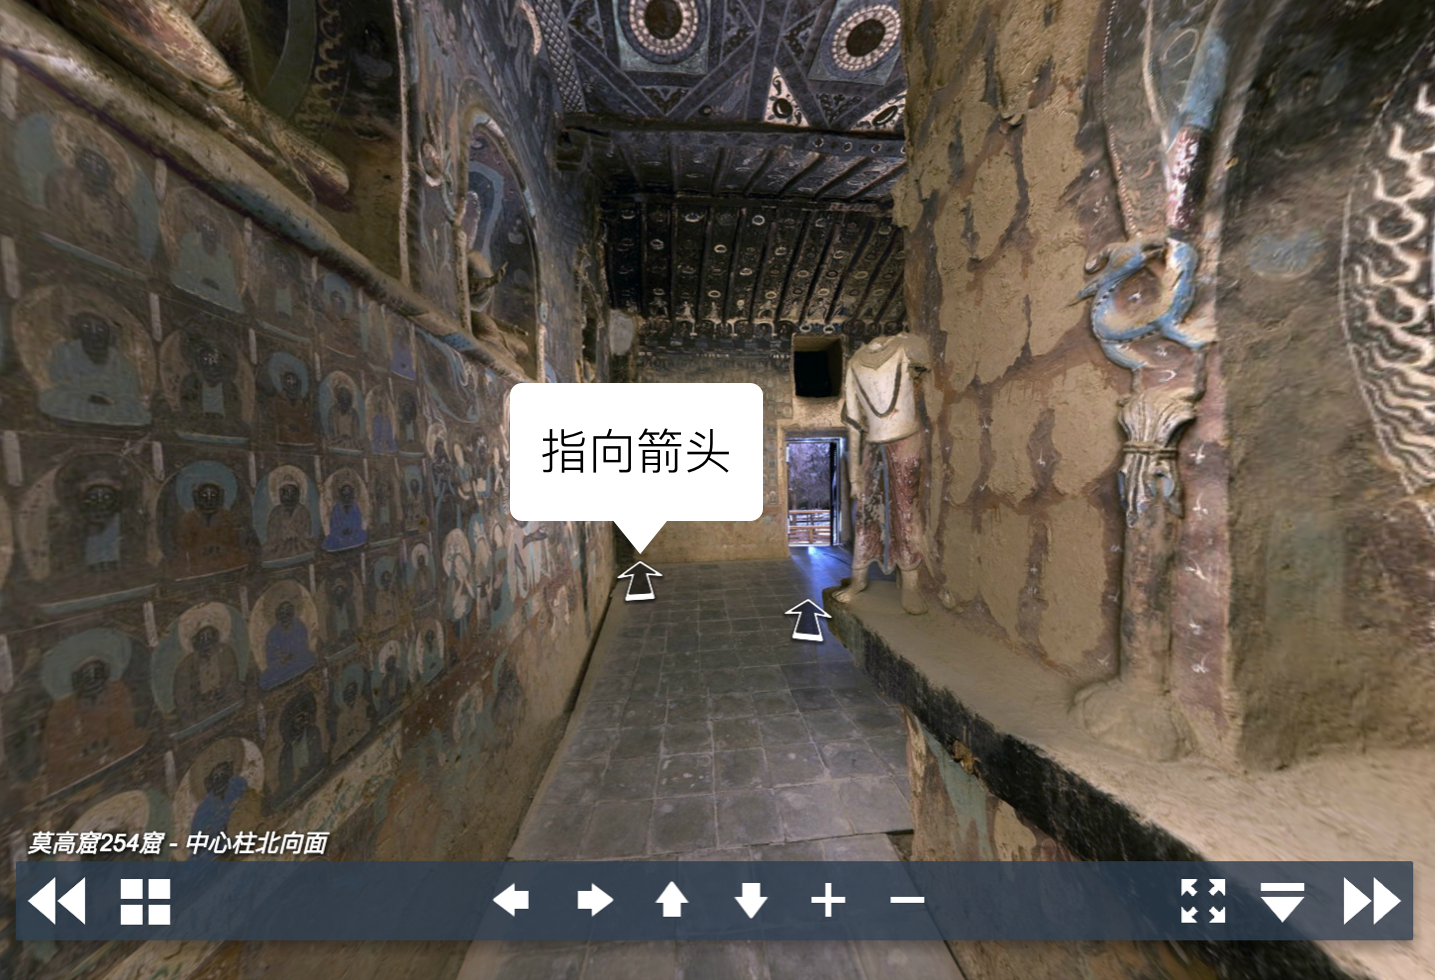
\includegraphics[width=.9\textwidth]{tip}
}
\caption{场景切换的指向箭头}
\label{fig:tip}
\end{minipage}
\begin{minipage}{.45\textwidth}
\centering 
\fbox{
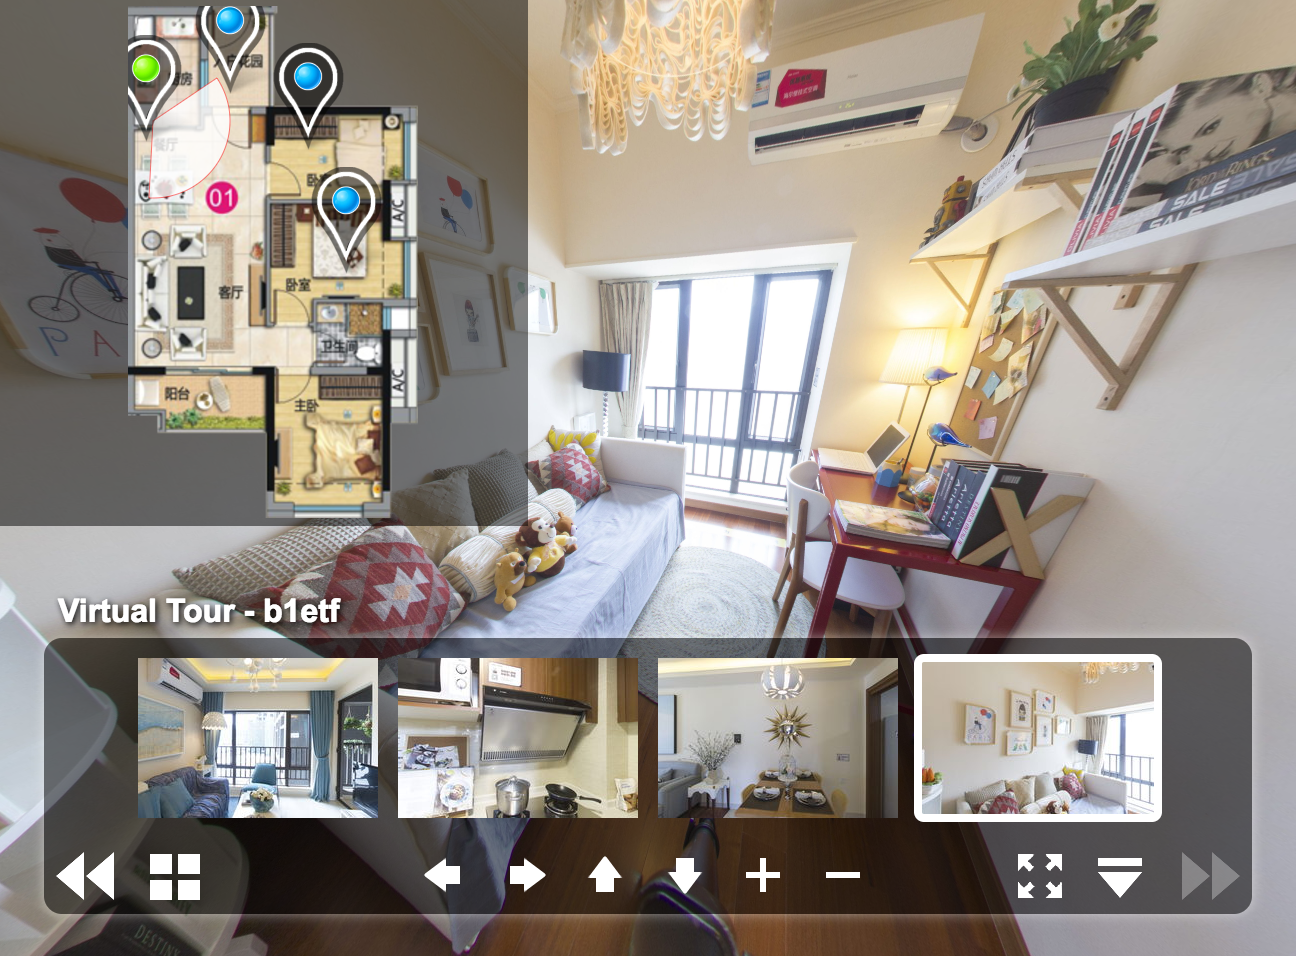
\includegraphics[width=.9\textwidth]{map}
}
\caption{场景小地图和场景序列}
\label{fig:map}
\end{minipage}
\end{figure}

针对上述问题,本文尝试使用一种改良过的指向图标来指示场景的出入和场景间的关系。如图\ref{fig:point}所示,图标的基本形态相同,均为带尖头的圆片状,不同的是其上面的标识随指示类型而不同。第一排为四种基本指向图标:普通指向、返回指向、付费指向和星标指向。

\begin{description}
	\item [基本指向图标] 以箭头作为标识,表示一般的场景切换
	\item [返回指向图标] 表示返回先前来源的场景
	\item [付费指向图标] 表示下一个为收费场景,需付费后才可进入
	\item [星标指向图标] 下一个场景为被推荐或用户自行标注为星标的场景
\end{description}

\begin{figure}[htp]
\centering
\fbox{
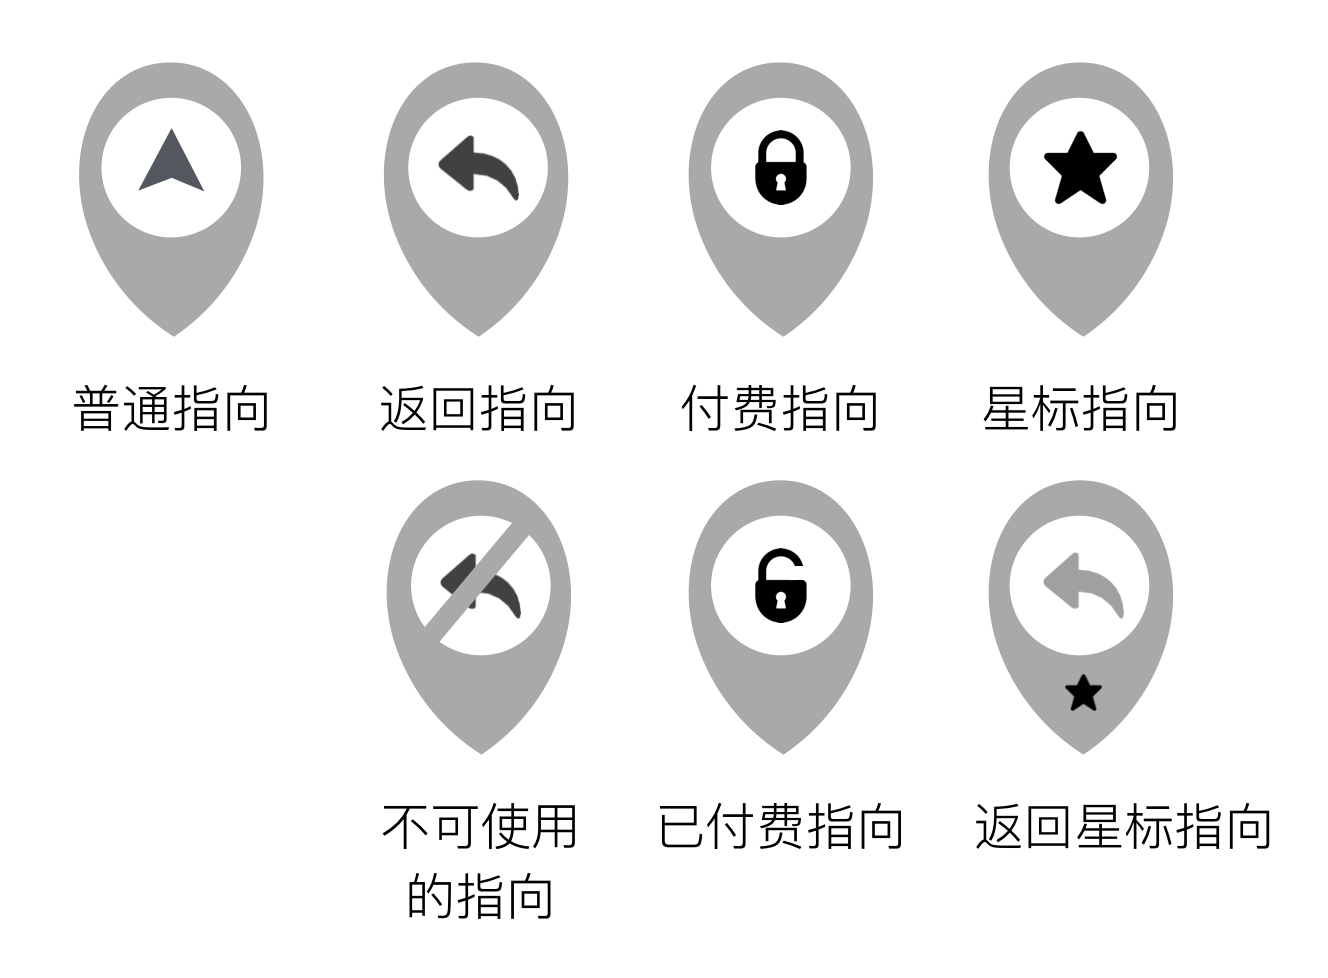
\includegraphics[width=.7\textwidth]{point}
}
\caption{新的指示图标系列}
\label{fig:point}
\end{figure}

图\ref{fig:point}第二排为依据第一排图标的形式异化得到的多指示图标。不可使用的指向图标表示该场景暂时不可用,已付费指向图标表示该场景已经付费可以正常使用,返回星标指向图标表示返回星标场景。这种图标形式可根据功能需求自由扩充组合使用,相比一般图标其携带信息量更大,用户可借此方便地确认想要前往的场景。

\subsection{直观化交互}
WYSIWYG,即“所见即所得”是一种常见的编辑模式,它便是一种很理想的设备交互模型,用户不必关注程序背后的逻辑,甚至不必关心自己编辑的文章真实存储的数据是何种形式,只需要看到屏幕上呈现的内容就是别人所能看到的内容。

全景漫游展示的正是这样一种过程,由不直观的概念转换为直观的概念。如图\ref{fig:wysiwyg}所示,人对房屋整体概念的认识观念是从具象至抽象,只有抽象简洁的概念才能方便地存储于人脑的记忆中,但涉及到具体房屋的理解时,是从单纯的“房屋”名词,到草图的展示,再到带有色彩的照片。

近年来,有学者提出基于物理存在感的交互设计,即在交互界面上模拟真实世界的物理实体,利用人生活中通过内隐性学习获得的缄默知识(即惯例和规则),从而带来产品易用性的提升和用户好感度的增强\endnote{徐冰,张翀,余永海. 基于直觉化的物理存在感交互设计研究[J]. 创意与设计,2011,(02):28-31.}。物理存在感是信息模式快速匹配,以求实现无需学习的直观化交互。全景漫游正是要物理存在感在计算机虚拟空间内的自然延续,延伸人类的心智世界,故将交互过程直观化为日常生活行为是可行的。

\begin{figure}[htp]
\centering
\fbox{
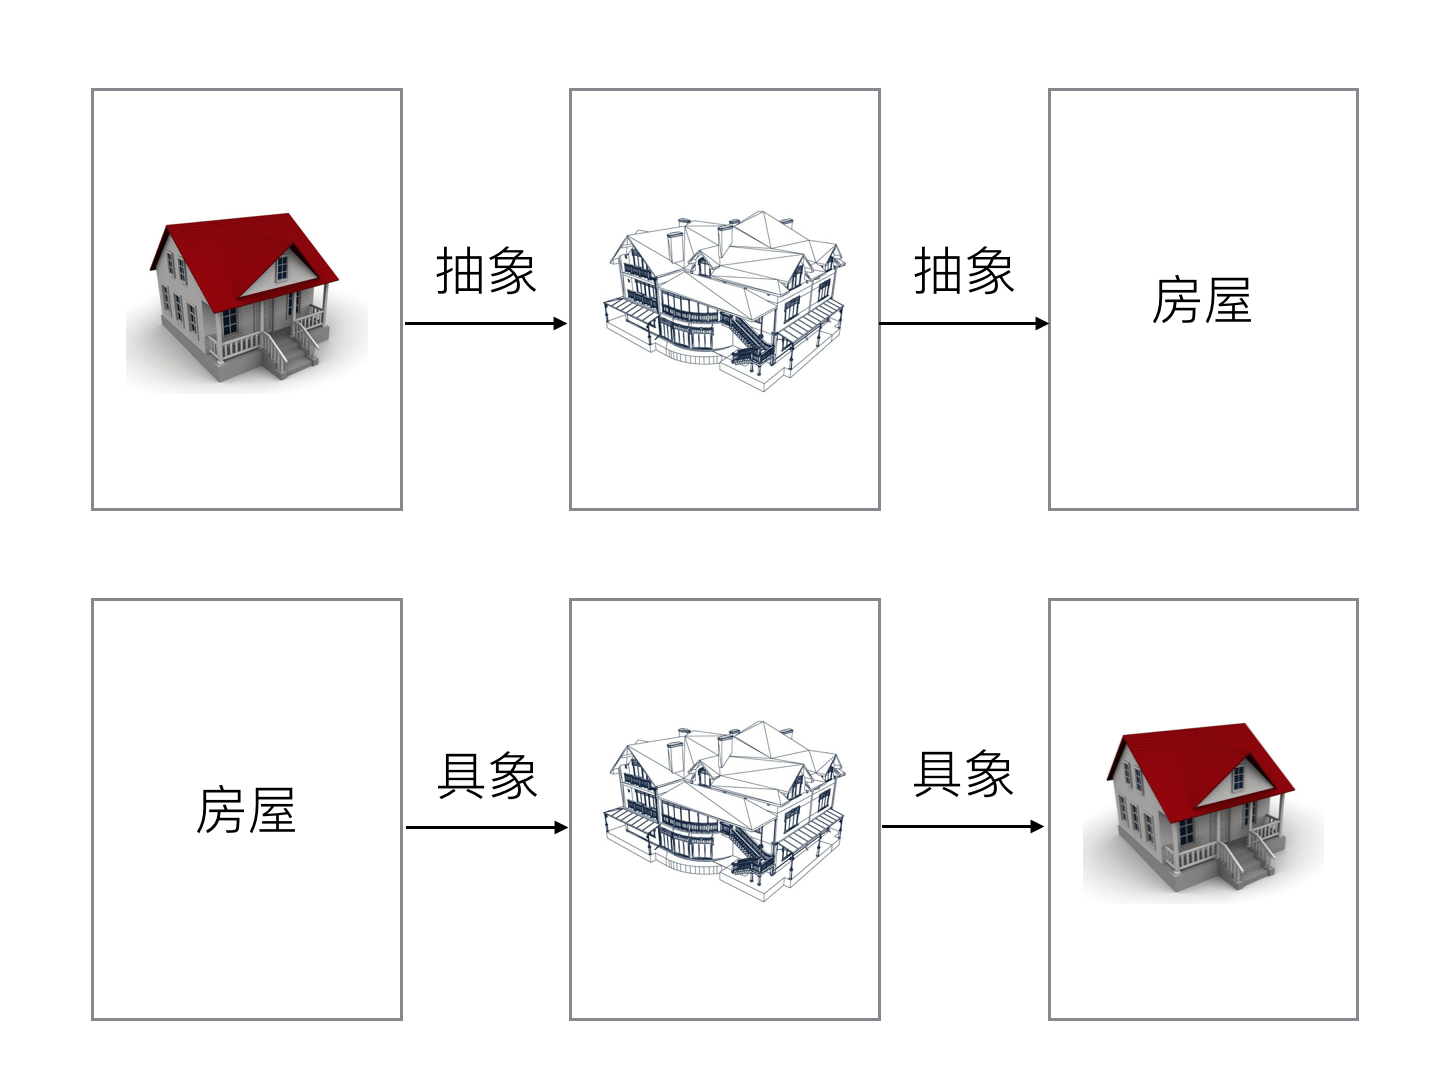
\includegraphics[width=.5\textwidth]{wysiwyg}
}
\caption{具象和抽象}
\label{fig:wysiwyg}
\end{figure}

本节主要从场景漫游路径、场景切换、直观化交互三个方面阐述了场景漫游状态下的交互模型。漫游路径的选取决定了全景漫游的连贯度;场景切换则是从设计角度弥补全景漫游的场景衔接直观性的不足,通过指示的方式提醒用户前后场景的特性和相互关系;直观化交互则是引入物理存在感的概念,将虚拟场景与真实场景结合起来,让用户可以凭借直接就能在场景里自如地漫游。根据上述分析,可以画出全景漫游场景相关的交互模型,如图\ref{fig:vr}。

\begin{figure}[htp]
\centering
\fbox{
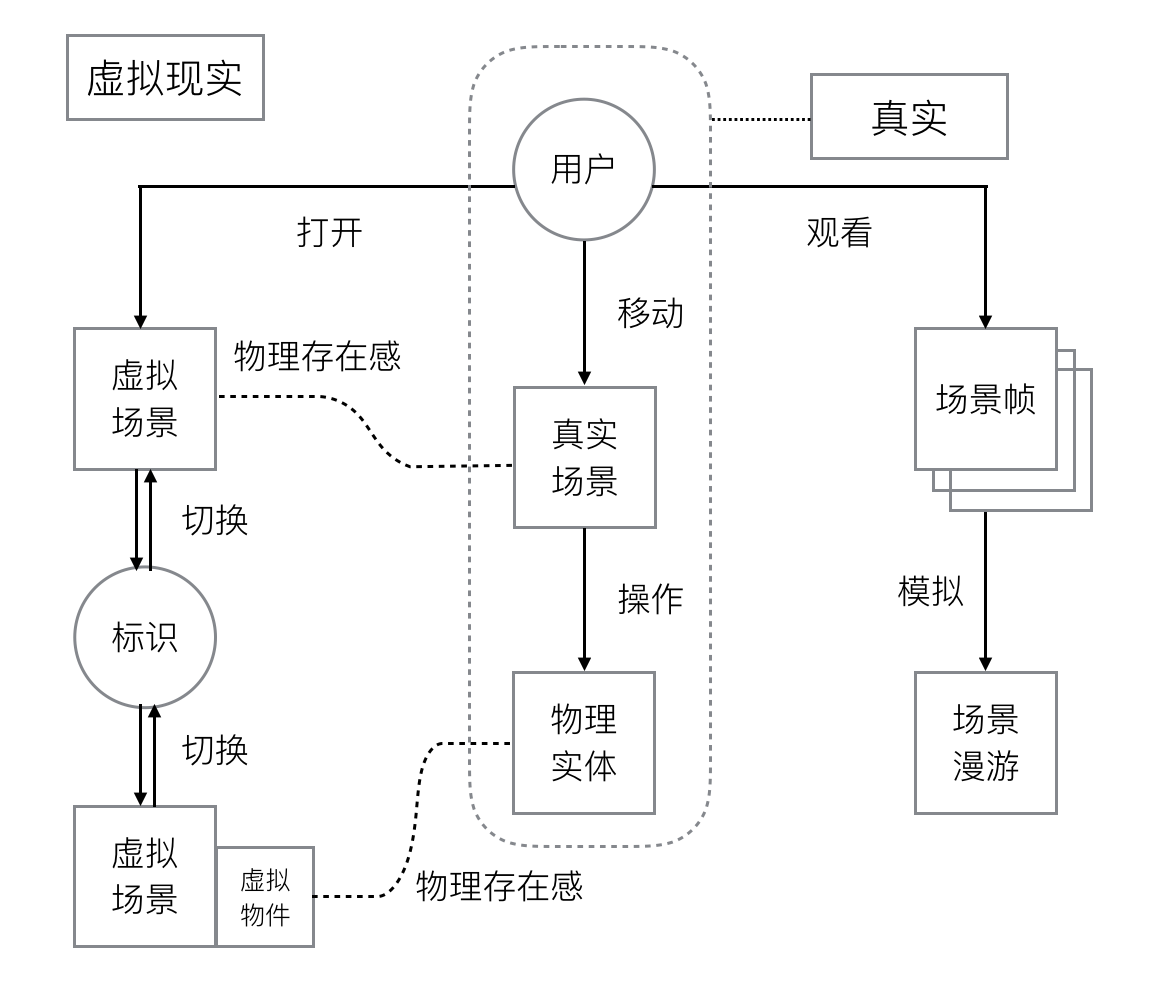
\includegraphics[width=.5\textwidth]{vr}
}
\caption{场景漫游的交互模型}
\label{fig:vr}
\end{figure}
  \chapter{全景漫游的可视化交互实践}
上文中通过对全景漫游与人的生理心理特性相互关系进行分析,梳理了以信息架构和功能模型为主导的可视化设计思路,为实际开发全景漫游项目奠定了基础。结合上述理论支持与作者实习实践所得经验,本章就作者在某公司进行实习工作时,进行全景漫游系统应用开发的过程为可视化交互示范案例进行分析。本案例将从需求定义、功能架构、交互模型定义出发,以实例开发为主线,通过界面设计和程序逻辑部分详细说明全景漫游的可视化实现过程,将理论与实践结合,从而提升全景漫游整体的使用交互体验。

\section{需求定义}
本例中的研究对象是个平台型的网络系统,网上商城类的应用,可通过供人浏览全景漫游的视频,体验商城全景漫游和购买。本项目在公司内部以 PC 端页面与移动端页面形式进行开发(作者参与设计与前端部分的开发,如图\ref{fig:woniu}),是涵盖全景场景视频采集技术、全景视频储存技术等开发内容的综合型全景漫游体验商业项目的衍生子项目之一。作者结合自身实践经历,提出了在开发传统网页界面等同时,利用网页技术直接开发基于 A-Frame 框架的全景漫游系统,将全景漫游的体验落实到用户进入应用到各个角落。该想法得到了作者实习时相关领导的认可与支持。因实习时间短暂,作者在公司完成了设计调研与传统网页界面的开发过程后结束了实习,此后独立继续开发并初步完成了全景漫游系统的原型设计与制作。

\begin{figure}[htp]
\centering
\fbox{
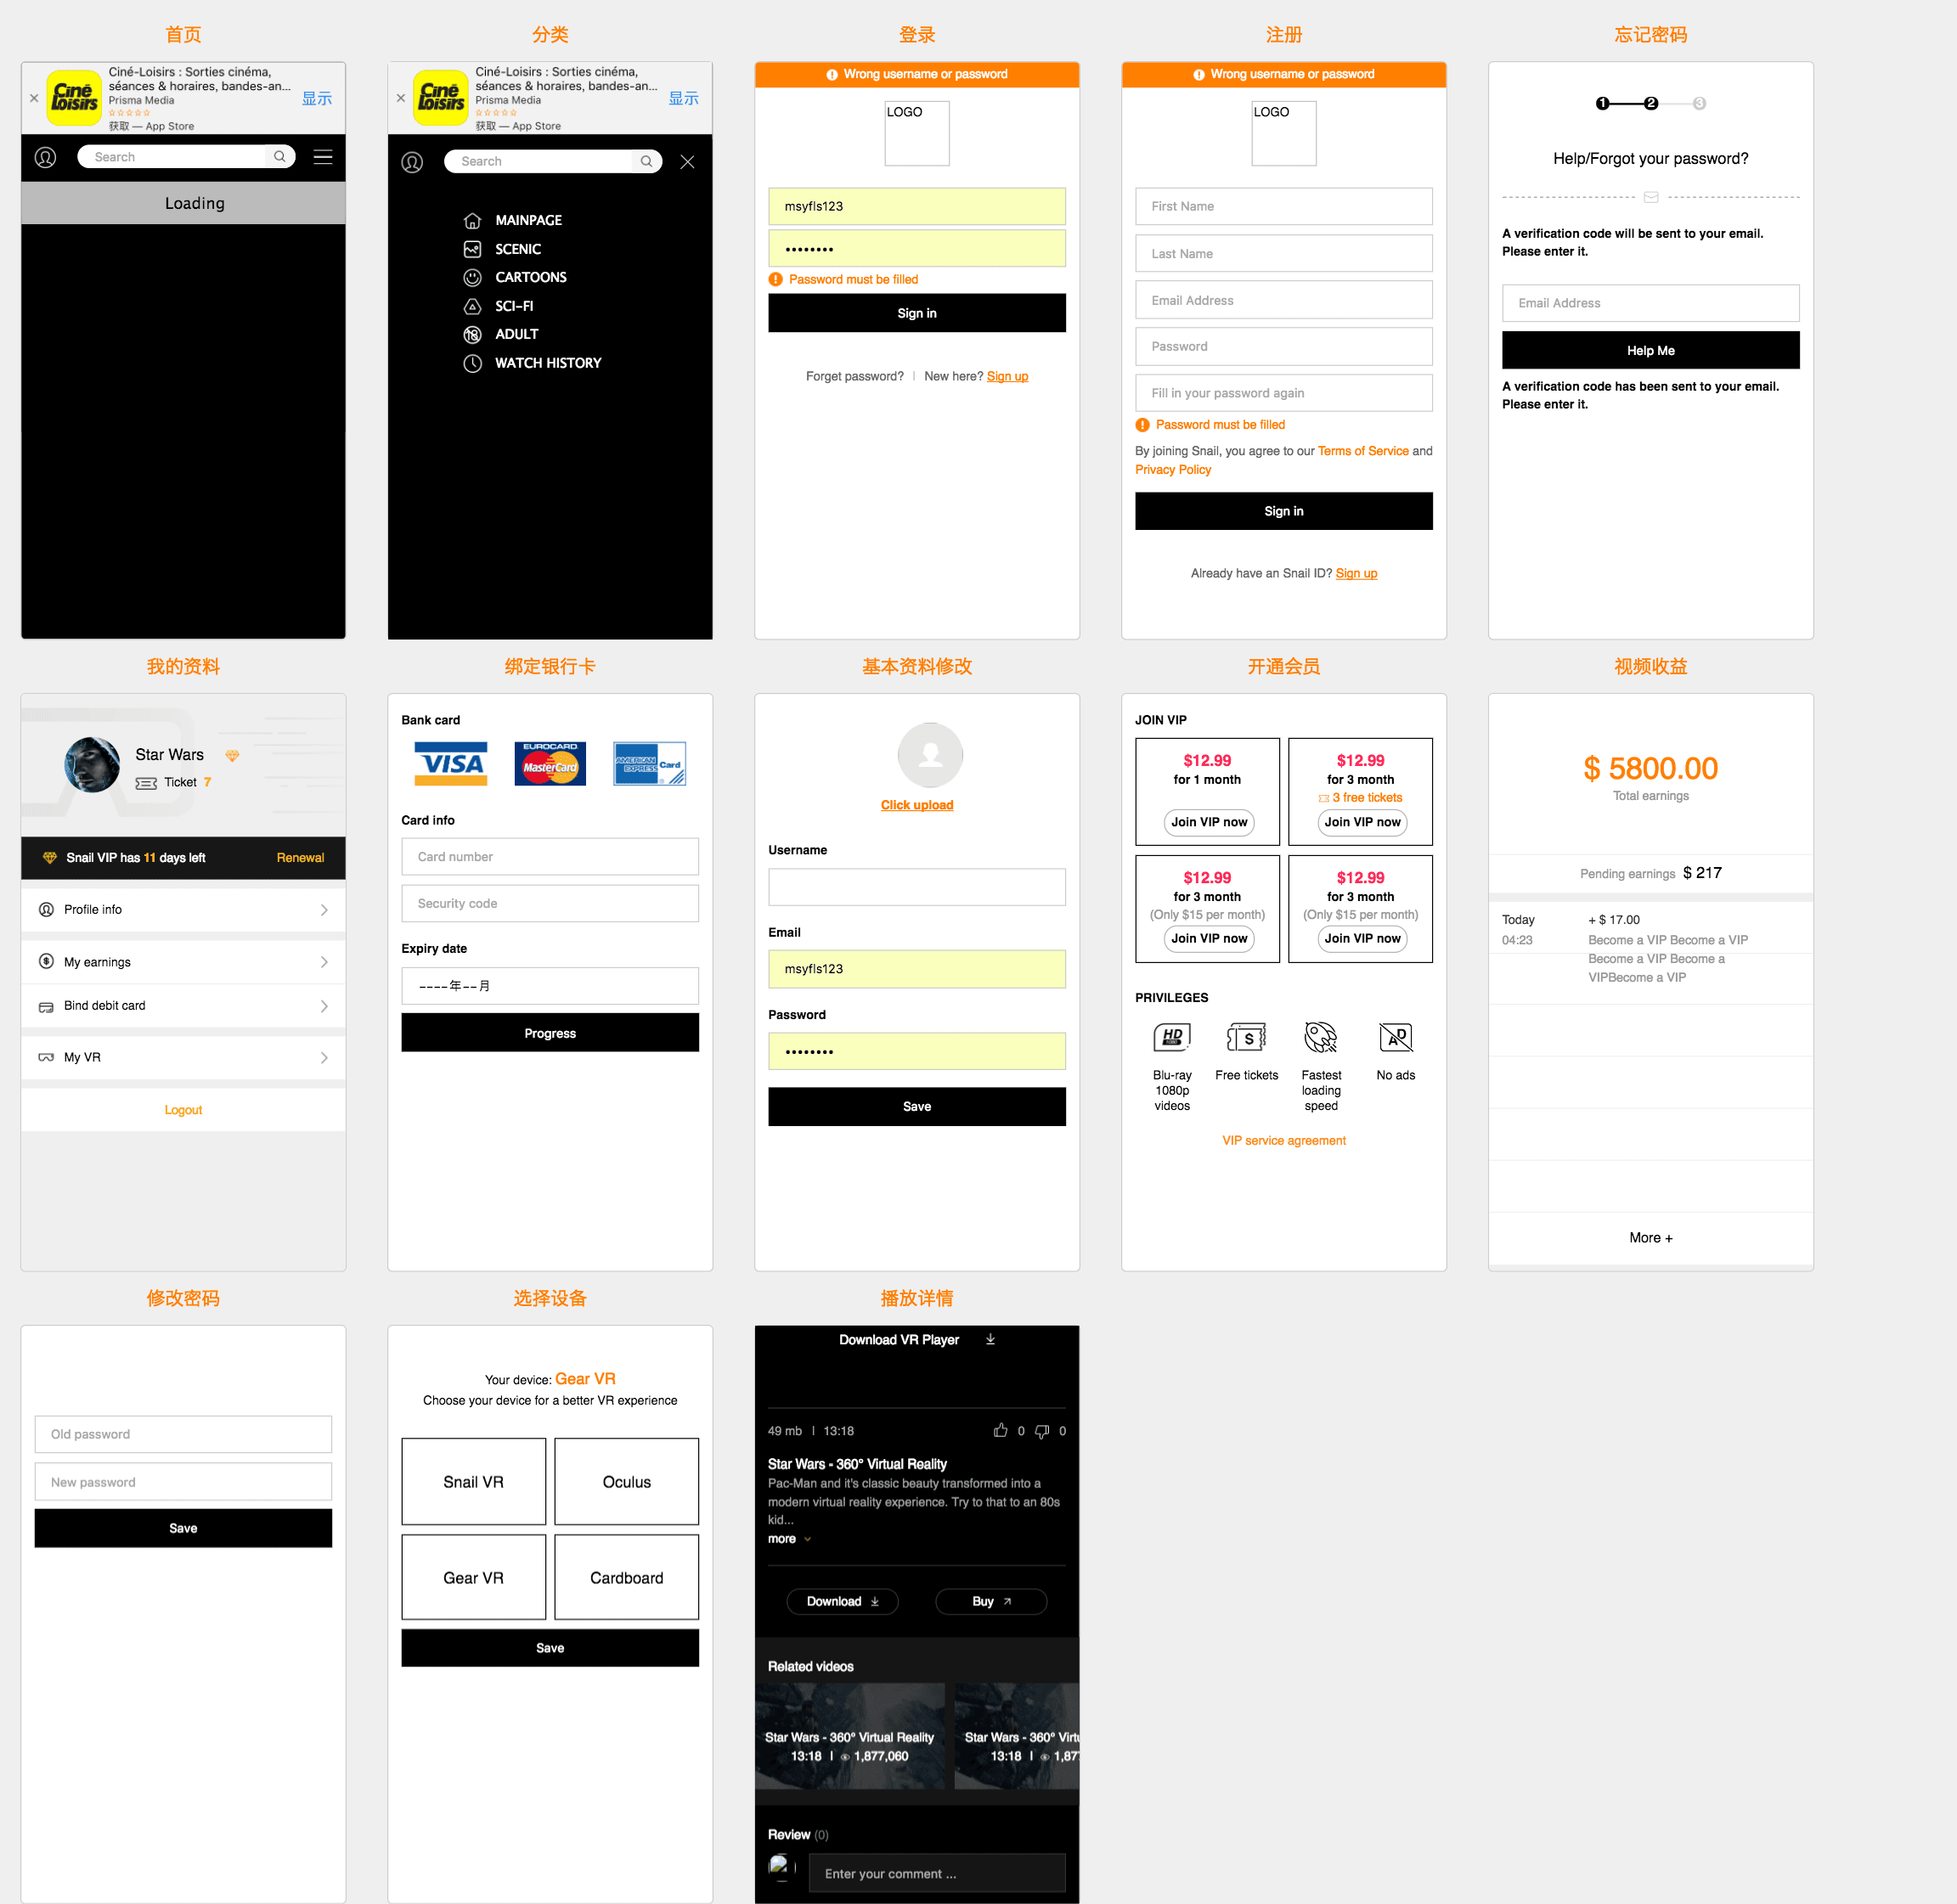
\includegraphics[width=.9\textwidth]{woniu}
}
\caption{移动端全景漫游系统原型}
\label{fig:woniu}
\end{figure}

需求列表如下:
\begin{enumerate}
	\item 满足基本全景漫游功能。因网页环境受限,以直接在浏览器内打开所支持的操作为限,暂不考虑开发多种操作形式功能。
	\item 带有商城功能,实现互动场景的付费/免费使用。
	\item 支持全景视频的播放,基本功能类似普通播放器。
	\item 带有基本的用户设置功能。
\end{enumerate}

根据以上原始需求,从价值需求、功能需求、数据需求等三个角度出发进行需求分析。

\subsection{价值需求分析}
该全景漫游系统的主要用户群为使用计算机或手持移动设备进行网页浏览的青少年群体。其用户特征为对新事物充满好奇心,愿意为良好的用户体验付出金钱成本,但缺点是对事物的专注度低,易于分心。

以该群体作为主要用户对象进行价值评估,按功能和用户的对应需求结合匹配,其价值需求如表\ref{tab:value}。

\begin{table}[htbp]
\centering
\caption{目标群体价值分析}
\vskip 5pt
\begin{tabular}{llll}
\toprule
功能点 & 用户需求 & 价值 \\
\midrule
新鲜感 & 体验到与其他应用不同的内容 & 高 \\
操作性 & 可以方便地了解并获取到所需体验的内容 & 中 \\
可信度 & 能够理解场景传达的信息并作出肯定答复 & 中 \\
丰富性 & 内容类别丰富、有不同难易层次可供选择 & 中 \\
可搜索 & 可以通过文本信息检索需要的项目 & 低 \\
可回溯 & 查看历史回放、收藏夹功能 & 低 \\
社交性 & 体验后愿意与别人分享使用体验 & 高 \\
\bottomrule
\end{tabular}
\label{tab:value}
\end{table}

根据分析,目标群体所期望的是一种不带有过多使用负担、随到随用、用完可离开也可进行分享的交互体验\endnote{陈圆. 手机应用软件界面体验设计研究[D].哈尔滨工程大学,2013.}
。

\subsection{功能需求分析}
据上述价值需求分析可得该全景漫游系统的功能需求,系统内的各种分类或是查找功能等,目的都是通过数据整理来让用户更好地发现场景并与其进行交互,如图\ref{fig:interaction}。经过整理分析以及结合软件开发难度等因素,可得功能需求表\ref{tab:func}。

\begin{figure}[htp]
\centering
\fbox{
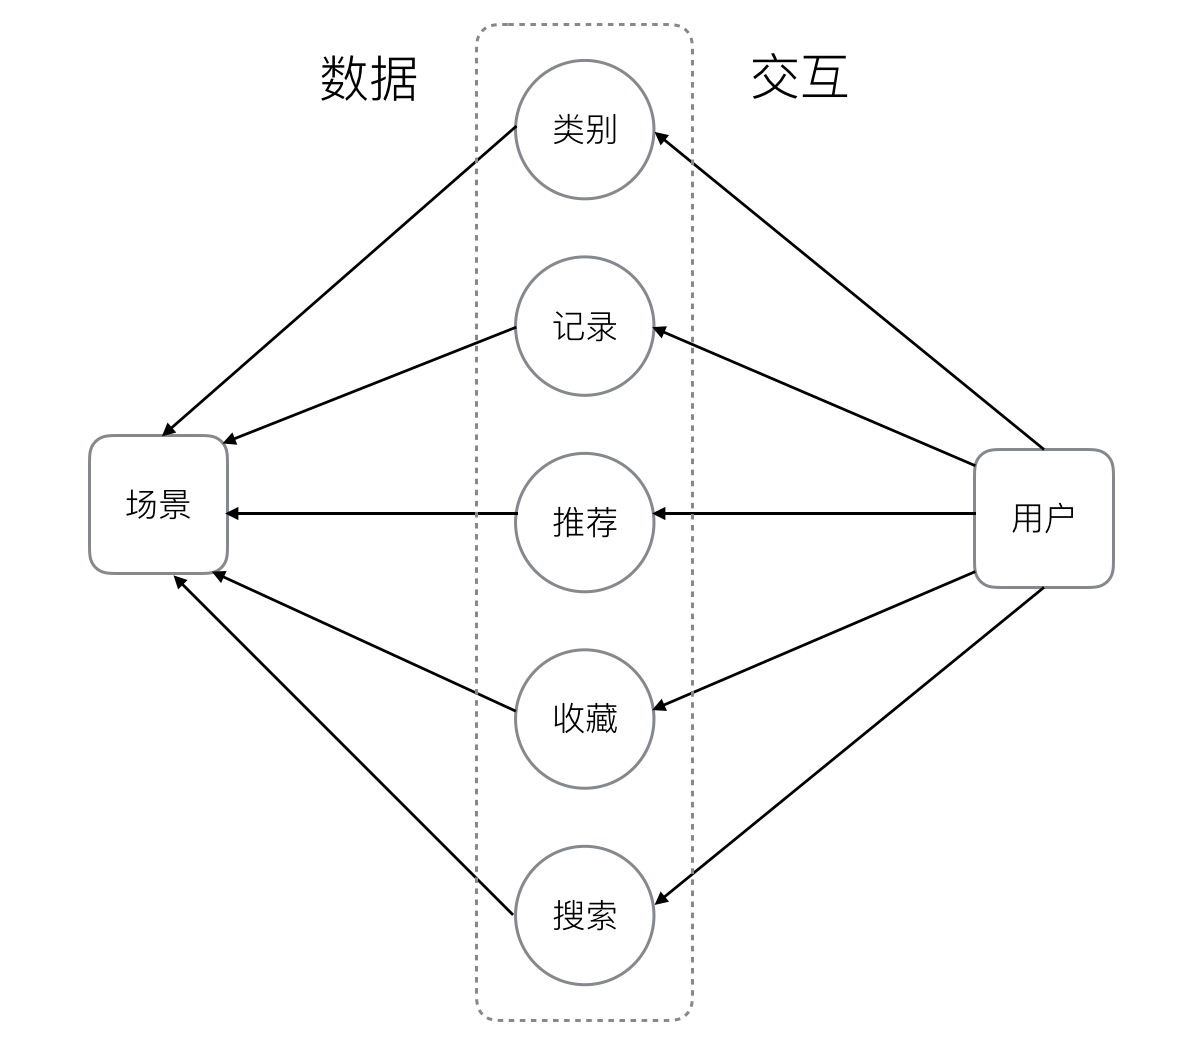
\includegraphics[width=.5\textwidth]{interaction}
}
\caption{用户通过多种形式发现场景}
\label{fig:interaction}
\end{figure}


\begin{table}[htp]
\centering
\caption{功能需求表}
\vskip 5pt
\begin{tabular}{lll}
\toprule
类别 & 功能点 & 描述 \\
\midrule
\multirow{3}{*}{主界面} & 推荐 & 进入推荐场景 \\
& 类别 & 按类别查看场景视频,可翻页,可进入类别界面 \\
& 应用 & 被固定的第三方开发的全景应用 \\
\midrule
\multirow{2}{*}{类别界面} & 列表 & 查看场景视频 \\
& 标签 & 切换类别 \\
\midrule
\multirow{2}{*}{应用界面} & 列表 & 展示第三方应用 \\
& 标签 & 切换类别 \\
\midrule
\multirow{2}{*}{设置界面} & 通用设置 & 提醒、关于 \\
& 个人偏好 & 账户设置、收藏夹、使用记录 \\
\midrule
\multirow{3}{*}{全局导航} & 返回 & 返回上一层 \\
& 主页 & 返回主界面 \\
& 搜索 & 唤起全局或当前类别搜索 \\
\midrule
\multirow{4}{*}{场景} & 定位 & 回到初始角度 \\
& 标签 & 标记为喜爱或讨厌、帮助改进推荐质量 \\
& 分享 & 分享页面至社交媒体 \\
& 解锁 & 解锁付费内容 \\
\bottomrule
\end{tabular}
\label{tab:func}
\end{table}

\subsection{数据需求分析}
根据上述功能需求可知,整个系统中最小的个体单位是场景,数据集合的建立是以场景为中心的。则该全景漫游系统的数据需求以单个场景的数据集出发,进行数据字段的定义,见表\ref{tab:data}。

\begin{table}[htp]
\centering
\caption{场景数据集}
\vskip 5pt
\begin{tabular}{lll}
\toprule
类别 & 字段 & 描述 \\
\midrule
\multirow{4}{*}{基础信息}& 名称 & 场景名称 \\
& 性质 & 视频、游戏、应用等 \\
& 标签 & 场景分类(如科幻、太空等) \\
& 介绍 & 场景简短介绍 \\
\midrule
\multirow{4}{*}{自然信息}& 容量 & 场景占用空间大小,以 kb 计 \\
& 创建日期 & 场景创建日期 \\
& 时长 & 仅对视频场景有效 \\
& 地理信息 & 场景录入地点 \\
\midrule
\multirow{3}{*}{人为信息}& 价格 & 免费、收费、部分收费 \\
& 分级 & 年龄限制、内容限制 \\
& 可用 & 可用或不可用 \\
\bottomrule
\end{tabular}
\label{tab:data}
\end{table}

而作为交互界面,场景是用来服务于使用其的用户的,故数据需求也包含用户信息数据的模型,见表\ref{tab:user}。

\begin{table}[htp]
\centering
\caption{用户数据集}
\vskip 5pt
\begin{tabular}{lll}
\toprule
类别 & 字段 & 描述 \\
\midrule
\multirow{3}{*}{基本信息} & 名称 & 账户名称 \\
& 密码 & 账户密码 \\
& 邮箱 & 账户邮箱 \\
\midrule
\multirow{3}{*}{被动收集信息} & 观看记录 & 场景、时间、时长 \\
& 付费记录 & 场景、应用、视频即其价格 \\
& 操作记录 & 使用场景的有效信息 \\
\midrule
\multirow{3}{*}{主动输入信息} & 标签 & 标记喜恶、收藏 \\
& 偏好设置 & 使用设备、情景模式等 \\
\bottomrule
\end{tabular}
\label{tab:user}
\end{table}

\section{功能架构}
据上述需求分析,该全景漫游系统等功能架构表现两种核心功能:“发现功能”和“场景漫游”。

\subsection{发现功能}
\begin{description}
	\item [浏览功能] 用户在包括主界面内的各种类别界面内浏览场景相关信息,发现自己所想要体验的场景。
	\item [搜索功能] 用户需要即时搜索得到自己想要的信息。
	\item [记录功能] 用户可以查看自己的浏览历史和收藏内容。
	\item [付费功能] 用户需要支付一定成本来查看某些场景或场景的局部。
	\item [自定义功能] 用户可以通过设置来自定义系统偏好。
\end{description}

\subsection{场景漫游功能}

\begin{description}
	\item [漫游功能] 用户可以通过转向、仰头低头、注视等方式漫游整个场景。
	\item [互动功能] 用户可以通过转向、仰头低头、注视等方式漫与场景内特定物件进行互动。
	\item [视频功能] 用户可以以全景的形式观看特殊全景视频。
	\item [标记功能] 用户将场景标记自己的评价、收藏或是分享给其他人。
\end{description}

\section{交互模型}
交互模型即是一系列交互方式、模式、行为的总称,它定义了交互过程中交互的主体对象和行为方式。交互模型并没有准确的定义,因为根据不同的产品而言,交互行为的目的并不相同。例如,对于网站管理员而言,编写并输入网站内容是使用网站的目的,而对于一般浏览者而言,浏览网页上提供的信息则是其在该网站上行为的目的,故从不同角色和视角看待交互模型都会是不同的。而构建交互模型的主要目的则是指导交互设计的进行,则构建一个能同时被用户接受并符合一般软件开发规律的交互模型是十分重要的。

交互模型需要符合用户心智模型并在后续可以方便进行扩充。全景漫游的场景交互模型在前一章节末尾处已经给出,此处不再赘述。在该全景漫游系统中,其系统交互模型如图\ref{fig:scene}。

\begin{figure}[htp]
\centering
\fbox{
  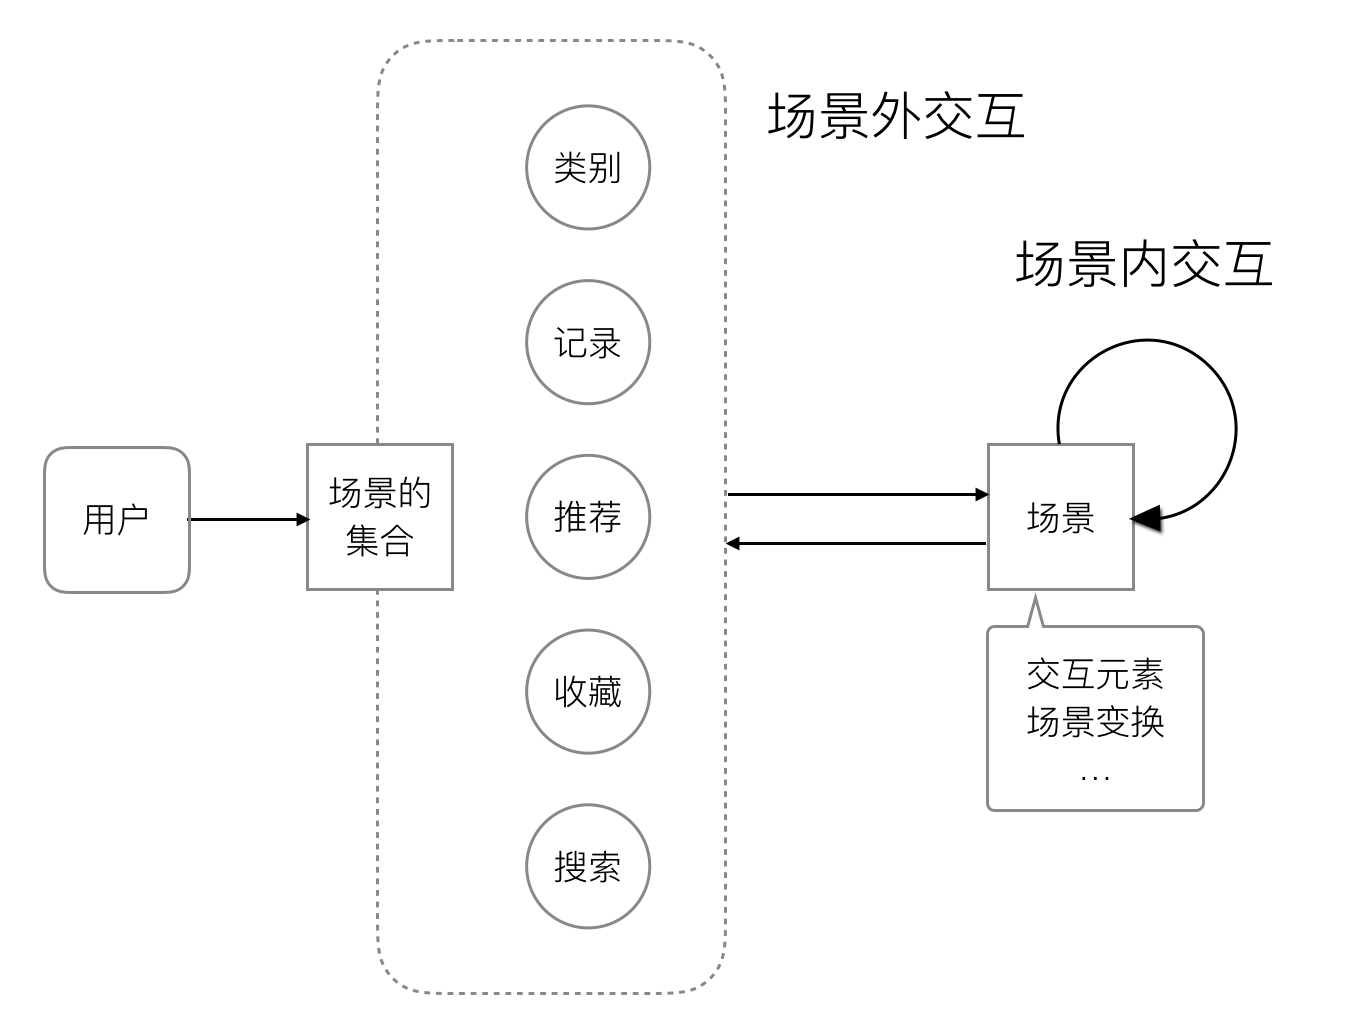
\includegraphics[width=.5\textwidth]{scene}
}
\caption{全景漫游系统的系统交互模型}
\label{fig:scene}
\end{figure}

\section{原型设计}
基于本文提出的全景漫游可视化交互模型,结合上述需求分析与功能架构,我们设计了一个基于网页技术、以开源框架 A-Frame 作为载体的网页版全景漫游系统作为设计原型进行设计制作并验证理论的有效性。

本文将着重从全景漫游系统的导航界面、场景界面、一般功能界面和操作方式等四个方面阐述该设计。
\subsection{类别界面设计}
上方为类别菜单,下边横长条为标签栏,可切换分类。底部为通用导航栏。如图\ref{fig:menu}。

\begin{figure}[htp]
\centering
\fbox{
  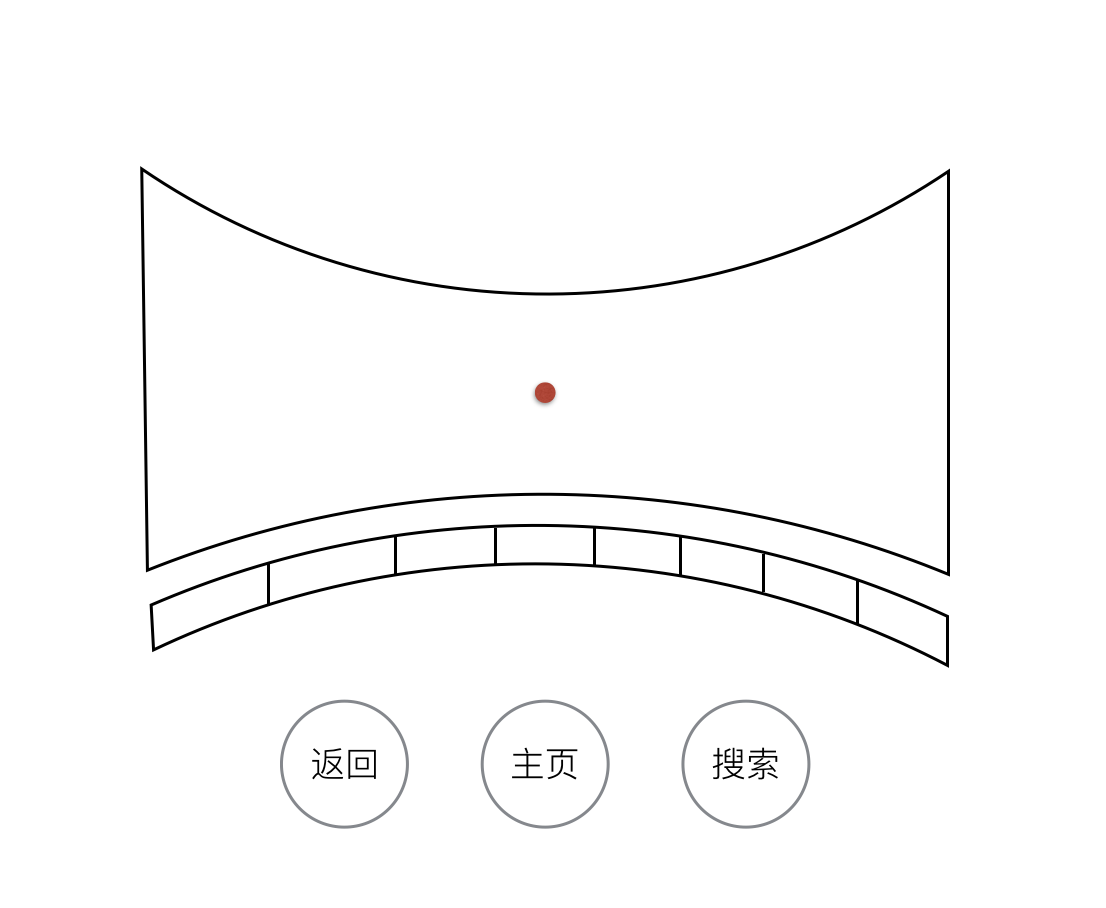
\includegraphics[width=.5\textwidth]{menu}
}
\caption{类别界面设计}
\label{fig:menu}
\end{figure}

\subsection{漫游界面设计}
\begin{itemize}
	\item 漫游界面带有紧急退出区域,只需注视 1~2 秒以上就可以紧急退出场景,避免眩晕加重。
	\item 可通过地面上的指示图标切换场景。
	\item 可通过场景中的热点区域查看详细信息。
\end{itemize}
如图\ref{fig:scenery}。

\begin{figure}[htp]
\centering
\fbox{
  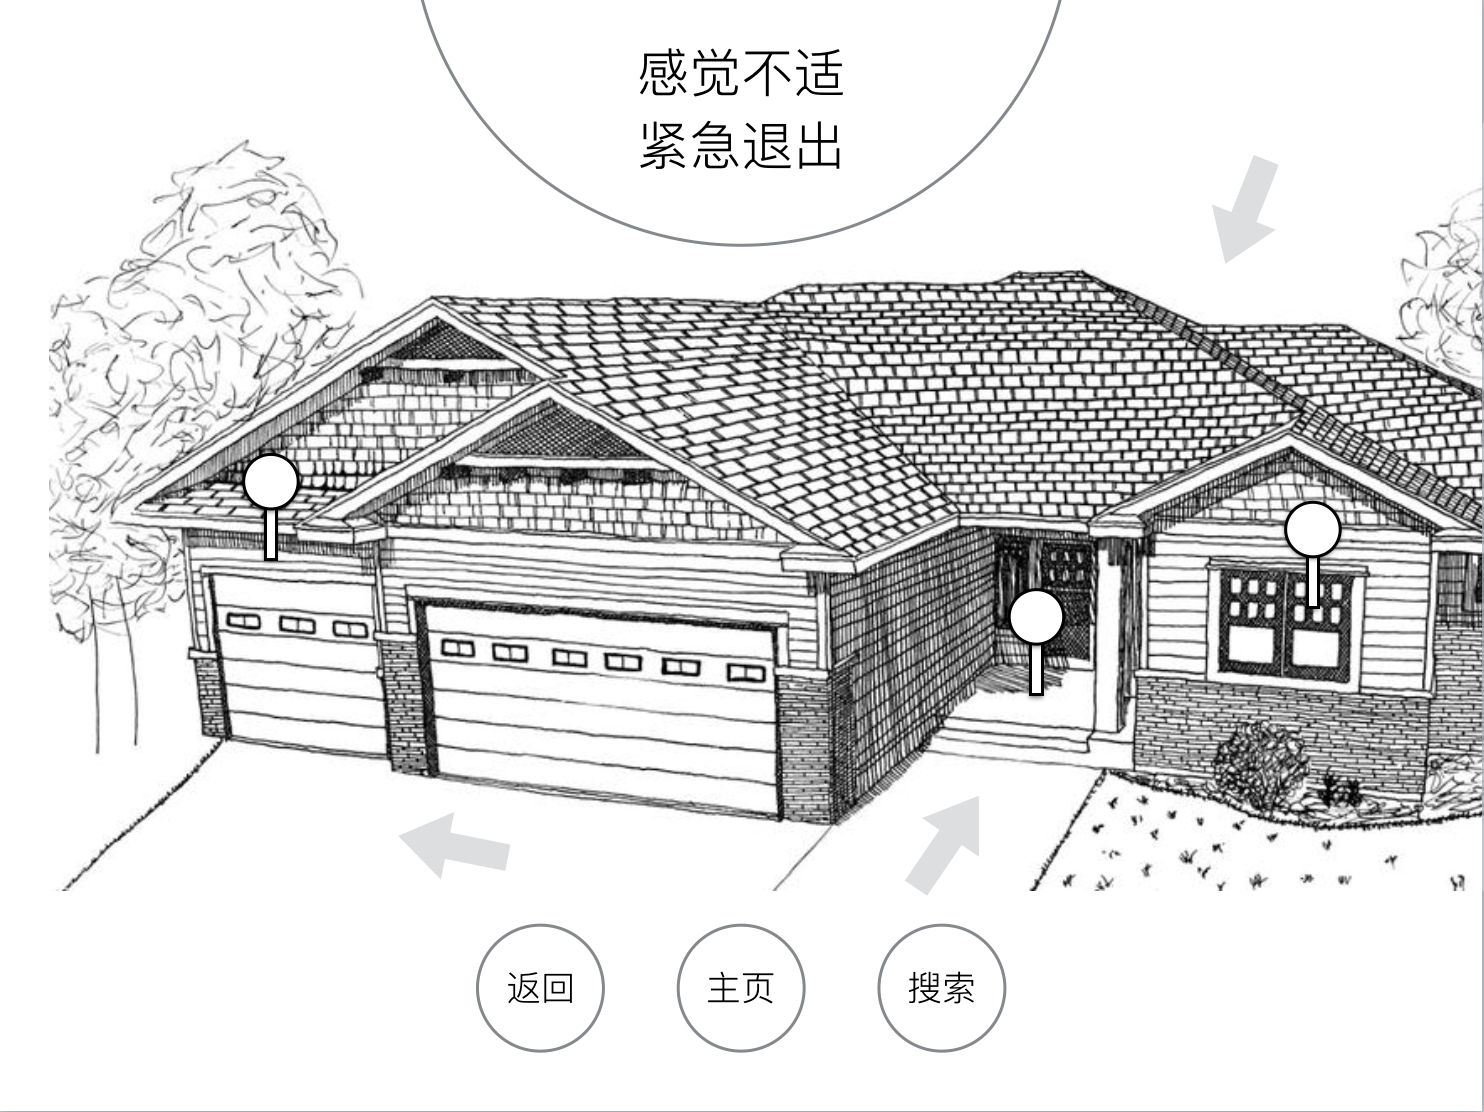
\includegraphics[width=.5\textwidth]{scenery}
}
\caption{漫游界面设计}
\label{fig:scenery}
\end{figure}

\subsection{设置界面设计}
设置界面可通过注视相关范围控件以调节参数,如图\ref{fig:setting}。

\begin{figure}[htp]
\centering
\fbox{
  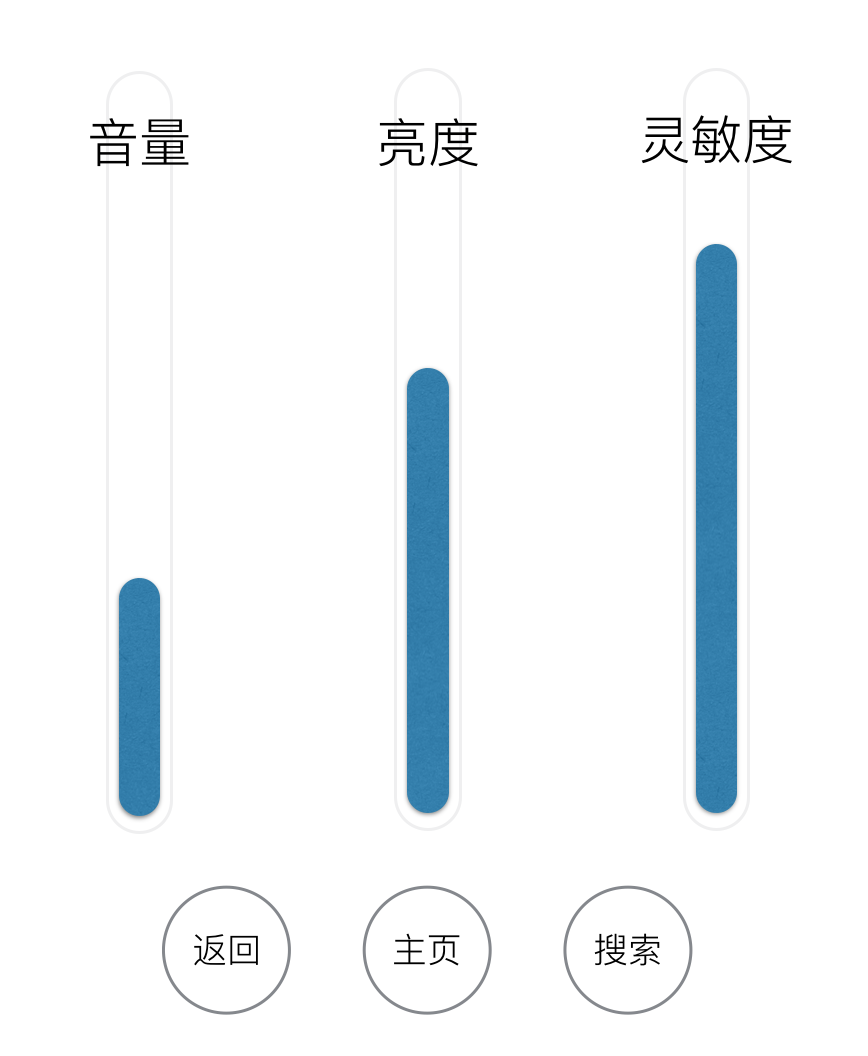
\includegraphics[width=.5\textwidth]{setting}
}
\caption{设置界面设计}
\label{fig:setting}
\end{figure}

\subsection{未完待续}

\section{程序示例}
本全景漫游系统采用 Mozilla 开源的 A-Frame 框架进行开发,可满足普通计算机及移动设备通过浏览器进行使用。

A-Frame 是一款由 Mozilla 开源的网页上用于创建实时虚拟现实体验的框架,其特点是封装性好,功能文档齐全且接受广大开发爱好者共同共享代码\endnote{Srushtika Neelakantam, Tanay Pant. Introduction to A-Frame[J]. 2017.}。其基本实现原理基于现代 HTML5 语言中的画布(Canvas)对象,通过调用底层系统实现高效率的 WebGL 绘图。画布对象的刷新率和延展性均符合全景漫游所必需的基本开发条件,且开发语言与一般网页开发技术类似,对开发团队较为友好,故选用其作为原型展示的应用平台。

开发后生成的原型文件可以通过普通网页进行访问,更可通过 Google Cardboard 配合手机实现简易的全景漫游,其开发便利且容易实现验证。借助以上技术及全景漫游可视化交互理论成果,用户可以真实感受到全景漫游技术带来的体验升级,能够以直观的交互形式与虚拟场景内的事务进行互动,切身体会科技带来的益处\endnote{张小超,王精业. 虚拟场景漫游系统的体系结构分析[J]. 系统仿真学报,2005,(04):917-919.}。
\subsection{示例代码}
实现一个简单的可用鼠标或注视(Fuse)操作的小场景。


\emph{HTML}
\begin{lstlisting}[language=HTML]
<a-scene>
  <a-entity
    id="box" cursor="fuse:true;fuseTimeout:1000"
    geometry="primitive: box"
    material="color: blue">
    <a-box
      src="img/logo.jpg"
      position="0 3 -5"
      rotation="45 0 45"
      scale="2 2 2"
      id="box1">
      <a-animation
        attribute="position"
        begin="focus"
        to="0 2.2 -5"
        direction="normal"
        dur="2000">
      </a-animation>
    </a-box>
  </a-entity>

  <a-camera>
    <a-cursor></a-cursor>
  </a-camera>

  <a-plane 
    position="0 0 -4" 
    rotation="-90 0 0" 
    width="4" 
    height="4" 
    color="#7BC8A4">
  </a-plane>
  <a-sky color="#ECECEC"></a-sky>
</a-scene>
\end{lstlisting} 

\emph{JavaScript}
\begin{lstlisting}{language=JavaScript}
document.querySelector('#box').addEventListener('click', function(e){
  document.querySelector('#box1').emit('focus')
})
\end{lstlisting}

  \chapter{全景漫游设计评价}

全景漫游的应用场景不同于普通二维界面,其操作方式也于一般应用大相径庭,故设计评价体系也应针对一般应用相应调整。设计评价的基本形式可分为定性分分析和定量分析两种。定性分析主要用于确定事物的不易被量化的特性,带有人较强的主观思维过程。定量分析用以确认事物间某些因素或具备性质间数量上的关系,受人主观意愿影响很小,故能够较为客观地反映事物间的相对联系。

在全景漫游可视化设计中,以上两种评价方式都是十分必要的,通过定性分析可以了解到用户自身对产品的使用感受与意愿建议,而定量分析可以将交互过程拆分成独立的操作步骤、更准确地定位设计中不合适的细节所在。下文将首先介绍交互指标的涉及范围,然后细化为面向用户的评价指标用以定性分析交互的优劣性,以操作过程的量化指标分析交互形式的合理性和效率。

\section{适用于全景漫游的交互指标}
根据前文全景漫游与人的关系一章所提出的观点,全景漫游的交互质量与人的生理及心理特征均有所关联,交互指标的确定也因涵盖上述两者。全景漫游与人的生理特性间交互的质量可以体现为用户操作的便利性,如操作动作幅度是否过大、复杂任务操作的步骤是否过多、需要集中注意操作的时间是否过长等。全景漫游与人的心理特征间交互的质量可以体现为用户对交互过程的满意度,表现为用户是否可以直观地理解场景意图、是否能够自主完成预期任务、是否能够自行解决遇到的问题等。

全景漫游的交互指标以生理和心理简单划分罗列,如表\ref{tab:interaction}。

\begin{table}[htp]
\centering
\caption 全景漫游交互指标
\vskip 5pt
\begin{tabular}{lll}
\toprule
类别 & 内容 & 参数\\
\midrule
\multirow{4}{*}{生理指标} & 视力、视野、色觉、听觉 & 视野宽度、色觉分辨力 	\\
& 触觉、温度、震动 & 温度、震动频率、频次 \\
& 肢体活动范围 & 头部活动范围 \\
& 人体舒适度、疲劳度 & 连续工作时长 \\
\midrule
\multirow{4}{*}{心理指标} & 易用性 & 操作时间、出错率 \\
& 愉悦性 & 用户满意度  \\
& 参与性 & 用户交互覆盖率  \\
& 接受性 & 用户满意率  \\
& 可靠性 & 用户满意度  \\
& 任务完成度 & 用户满意度  \\
\bottomrule
\end{tabular}
\label{tab:interaction}
\end{table}

\section{面向用户的评价指标}
面向用户的评价指标以定性评价为主,主要用于采集用户使用过程中的主观感受及反馈。为简化用户填表时的考量因素,以 1-5 级等级策略统计为标准进行问卷设计\endnote{姜强,赵蔚,王朋娇. 自适应学习系统中双向适应交互评价实证研究[J]. 现代远程教育研究,2013,(05):106-112.}。其中,1 级为非常不同意, 2 级为较不同意, 3 级为一般同意, 4 级为较同意, 5 级为非常同意。调查问卷如下表\ref{tab:questionnaire}。

\begin{table}[htp]
\centering
\caption 使用问卷
\vskip 5pt
\begin{tabular}{lcl}
\toprule
类别 & 序号 & 问题 \\
\midrule
\multirow{5}{*}{心理指标} & 1 & 我对该系统容易上手(\enskip) \\
& 2 & 我使用后感到愉悦(\enskip) \\
& 3 & 我有参与其中的感觉(\enskip) \\
& 4 & 我有继续使用该系统的意愿(\enskip) \\
& 5 & 我认为该系统是可靠耐用的(\enskip) \\
\midrule
\multirow{4}{*}{生理指标} & 6 & 我使用后感到疲劳(\enskip) \\
& 7 & 我使用后眼睛感到不舒服(\enskip) \\
& 8 & 我觉得头部不舒服(\enskip) \\
& 9 & 我觉得使用后很热(\enskip) \\
\bottomrule
\end{tabular}
\label{tab:questionnaire}
\end{table}

\section{操作过程的量化指标}

用户在操作全景漫游系统时也应进行记录其操作过程,得到的操作数据能够真实地体现用户在操作过程中的使用状态;对于一些不可复现或通过回忆记起的操作细节而言,通过使用记录能够更真实地反映出来。并且,在使用过程中因没有外在提示提醒,用户能够反映真实的使用习惯,也可以暴露更多的设计问题。

考虑到量化指标的特性与实际操作的可行性,量化指标的收集应注重效率,在设计验证过程中关键位置收集的若干参数好于全局收集的普遍参数。同时,在调查具有针对性的指标时也应注意指标的客观性,避免因主观原因导致的测量误差存在。

经作者整理,一些较有代表性的可测量数据如表\ref{tab:questionnaire}。

\begin{table}[htp]
\centering
\caption 使用过程量化指标
\vskip 5pt
\begin{tabular}{lll}
\toprule
序号 & 问题 & 数据 \\
\midrule
1 & 用户初次打开页面至进入第一个场景的时间 & 	\\
2 &  用户在第一个场景中停留的时间 & \\
3 & 用户第一次学会使用视线停留触发物件效果的时间 & \\
4 & 用户触发全局导航栏内任一功能时间 & \\
5 & 用户是否分享、分享到何处 & \\
6 & 用户是否第二次打开应用、相隔时间 & \\
7 & 用户有无打开多个应用或场景、个数 & \\
\bottomrule
\end{tabular}
\label{tab:questionnaire2}
\end{table}

针对上述数据,第 1 项为用户完成一个有效导航操作的所用时间,可以反映导航功能的完善程度,侧面体现应用的易用性;第 2 项用户停留时间,能够反映用户的舒适度;第 3 项学习所用的时间可以反映系统中交互操作的易学程度;第 4 项导航功能可以反映用户对场景的参与度;第 5 项分享功能能够反映用户对应用的接受度和愉悦感;第 6、7 项是否再次使用可以反映用户对应用的接受度。

根据全景漫游应用的类别,上述指标可相应调整或增删。基本原则是测量用户真实的使用过程数据,以求反映交互设计的完成度和功能完整性。


\section{交互评价示例}

本评价示例以全景漫游系统至全景场景的漫游过程为试用过程,通过程序设计中添加统计代码的形式获得第一手用户数据,同时通过问卷形式调查用户使用体验。本例调查以自愿形式抽取了容量为 20 人的样本。

\begin{table}[htp]
\centering
\caption 使用问卷数据
\vskip 5pt
\begin{tabular}{lcllllll}
\toprule
类别 & 序号 & 问题 
& \tabincell{c}{非常\\不同意\\(\%)} & \tabincell{c}{较不\\同意} & \tabincell{c}{一般\\同意} & \tabincell{c}{较同意} & \tabincell{c}{非常\\同意} \\
\midrule
\multirow{5}{*}{\tabincell{c}{心理\\指标}} & 1 & 我对该系统容易上手
& 0 & 1 & 12 & 5 & 2 \\
& 2 & 我使用后感到愉悦
& 0 & 0 & 14 & 3 & 3 \\
& 3 & 我有参与其中的感觉
& 6 & 2 & 2 & 7 & 9 \\
& 4 & 我有继续使用该系统的意愿
& 0 & 1 & 11 & 3 & 5 \\
& 5 & 我认为该系统是可靠耐用的
& 5 & 2 & 8 & 4 & 1 \\
\midrule
\multirow{4}{*}{\tabincell{c}{生理\\指标}} & 6 & 我使用后感到疲劳
& 2 & 3 & 6 & 5 & 4 \\
& 7 & 我使用后眼睛感到不舒服
& 0 & 2 & 6 & 8 & 4 \\
& 8 & 我觉得头部不舒服
& 1 & 0 & 3 & 9 & 7 \\
& 9 & 我觉得使用后很热
& 0 & 0 & 7 & 9 & 4 \\
\bottomrule
\multicolumn{8}{l}{\small{注:表中数据单位为百分比,数据取经四舍五入至百分位 }} \\
\end{tabular}
\label{tab:result}
\end{table}

\begin{table}[htp]
\centering
\caption 量化指标数据
\vskip 5pt
\begin{tabular}{lll}
\toprule
序号 & 问题 & 时长/个数 \\
\midrule
1 & 用户初次打开页面至进入第一个场景的时间 & 32.2 秒	\\
2 &  用户在第一个场景中停留的时间 & 57.3 秒 \\
3 & 用户第一次学会使用视线停留触发物件效果的时间 & 8.7 秒 \\
4 & 用户触发全局导航栏内任一功能时间 & 14.1 秒 \\
5 & 用户有无打开多个应用或场景、个数 & 1.3 个 \\
\bottomrule
\end{tabular}
\label{tab:questiondata}
\end{table}

上述数据显示,多数用户对全景漫游的体验表示满意,但认为使用该系统存在多项生理上的不适应,该系统的易用性和接受度仍不太高,但考虑到示例程序的简单性,接受度低是预料中的。用户操作过程基本顺利,但也有一部分用户需要经过指导后才学会使用凝视操作触发按钮等操作,可见无按键的交互形式可接受程度较低;用户在导航界面停留过程是较长的,但在场景中停留时间却没有达到 1 分钟的预期,可见场景内容的复杂度和深度尚未达到用户沉浸的标准。用户后续继续使用全景漫游的意愿不够强烈,大部分用户在 2 分钟前后就结束了全景漫游的过程,结合问卷中“感受到很热体验”的用户数量可以认识到全景漫游因其使用特殊性,易造成用户因刺激过大造成心理和生理的双重不适感受,故全景漫游设备的配戴形式仍需要改进以减轻长期使用的不适感。

总体而言,全景漫游中可视化交互设计理论的应用是符合设计预期的,用户经过一定的指导和提示后均能自主完成全景漫游的体验,这与良好的交互设计是密不可分的,同时也是因为全景漫游这种形式符合人本身的内隐性知识和日常惯例,操作方式能够很快被人理解。场景中指向标识的设置、位移控件、全局导航栏的设置等均对用户全景漫游过程产生了积极的影响,但不足的是场景应用的单一性令用户很难全面沉浸入场景,易感到疲劳,这一点或许与全景漫游没有实现视野的深度信息造成用户视觉特征信息的失调有关。
  \chapter{总结}

\section{主要工作与创新点}
本文在详细研究了全景漫游相关技术及市场现状的基础上,通过分析全景漫游与人的关系,针对现有全景漫游体验感和交互形式弱的问题,就以下内容进行了深入研究。

首先从全景漫游的技术特点入手,以人的视觉特征为对象分析并得出了全景漫游中视觉布局应偏下的特点。结合听觉中双耳效应的原理,论述了全景漫游中声音对视觉增强的辅助作用。全景漫游与人的肢体运动相结合分析,认识到全景漫游中漫游形式与感知设备的密切关系,并就全景漫游手部操控设备间进行了可用性方面的对比。阐述了全景漫游中“视觉辐辏”过程与适应性调节相冲突继而造成漫游中及漫游后晕眩的过程,提出减小物体间景深差距以缓解相关反应的设想。就全景漫游中意识的注意与持续集中方面进行论述,分析得出保持漫游中刺激强度和持续时间均衡以避免短时过强刺激影响使用的观点。通过双指缩放的案例说明记忆与思维在理解并记忆交互行为中的影响。

通过对可视化界面发展趋势的分析,表明了建立合理信息架构和交互模型的必要性。将全景漫游与真实世界的游乐场进行类比,阐述了熟悉的信息架构可以帮助用户更高效地交互的观点。从信息架构的三个组织方式:自顶向下、自底向上和不可见的组织形式出发,提出了信息架构组件化和可视化的观点,并借此建立全景漫游的基本功能模型:漫游、导航、搜索、记忆等。以部分特殊模块的设计为例,叙述了模块设计的规则特性,在多输入交互模块中提到了通过重力感应头部动作的形式可以进一步开发更多更适合全景漫游功能的交互形式。

针对全景漫游交互模型方面,以设备捕获的信息流为线索,举例说明了交互过程中等待反馈时间产生的原因与解决方法,并就信息修正的角度揭示了用户在交互过程中的主观能动性。通过对信息架构中三种组织形式的利用,构建了基于上下文感知、增强信息和多任务切换为基础全景漫游导航系统交互模型,提出了上下文语境中存在语境切换和小语境内部信息沟通的观点。通过阐述全景漫游中漫游路径形式的局限性,认识到场景切换中信息的表达性有待改善,提出了增强性场景切换标识的方式以实现场景中的直观化交互理念。

最后以某公司全景漫游系统开发为例,经过需求定义、功能架构定义和交互模型定义,通过定义常用术语帮助理解,并就导航界面、漫游界面和常用功能界面三个方面深入设计了全景漫游的应用原型。经过简单的程序开发,并经过分析采用了定性定量相结合的交互评价体系对用户主观评价和操作过程中的量化指标均提出了可行的评价形式,并以前文中设计的原型进行试评价,取得了一定的设计评价成果。

本文提出了以人为中心、可视化交互为主导的全景漫游交互设计思路,从人与全景漫游的关系至全景漫游中信息架构和交互模型的分析论证中分析了全景漫游交互设计中重点功能的实现与细节的处理,为全景漫游相关设计提供了相关分析思路和实践经验。

\section{有待改进的地方}
本文就全景漫游技术相关的可视化交互理论进行了详细的研究,提出了结合信息架构与交互模型的设计思路,并以实例开发为例进行实践和评价。基于本文基础可开展以下深入工作:
\begin{enumerate}
	\item 全景漫游中交互形式实现以现有技术为基础,但交互形似仍沿用计算机屏幕时代的交互特性,应提出更多适合可穿戴设备的多通道交互形式以增强交互的体验性。
	\item 本文提出的全景漫游交互模型应用场景为平台类的全景漫游应用,对单一应用的交互模型因应用场景限制不够深入,未来可针对特殊应用情形进行相应的扩展与补充。
    \item 本文实践部分采用的实现框架为 Web 方向,因作者对该方向技术较为熟悉,未来可借助本文中相关理论就其他平台全景漫游应用作相应衍生,希冀全景漫游技术得到更多平台的更多支持!
\end{enumerate}

%%%%%%%%%%%%%%%%%%%%%%%%%%%%%%
%% 附件部分
%%%%%%%%%%%%%%%%%%%%%%%%%%%%%%
\backmatter
  \makeatletter
  \ifustc@bachelor\relax\else
    % 致谢
    % !TEX root = ../main.tex
\begin{thanks}

作者研究生就读期间得到了各位老师同学的悉心帮助与指导,谢谢你们让我成为一个更好的人!

首先,感谢我的导师周晔老师,周老师从本科起就担任我们专业相关课程的授课老师,课堂上对学子淳淳教诲、言传身教,在科研上精益求精、指导我们向学术领域高峰奋进。在毕业论文开题至写作完成期间,周老师均给予了我莫大的帮助,对论文中存在的问题详细解答,使我受益匪浅。

然后,要感谢本专业其他各位老师。蔡建平老师于本科时指导我参加某全国比赛并收获佳绩,知遇之恩没齿难忘;陈晓鹂老师与我成为了科研学习方面良好的合作伙伴,一起完成了一个又一个科研实践项目;顾湘老师对我严格认真,我于研一时参与顾老师的助教工作感到十分荣幸。还有李理老师、肖畅老师、杨展老师等在我学习期间给予的帮助与支持,谢谢你们!

最后,感谢同寝室的兄弟、专业内其他同学以及我的家人,你们是我生活上最好的伙伴和后盾。

\vskip 18pt

\begin{flushright}

~~~~马申彥~~~~

\today

\end{flushright}

\end{thanks}
%硕博致谢部分
    % 发表文章目录
    %\include{chapter/pub}
  \fi
  \makeatother
  % 参考文献
  % 使用 BibTeX
  % 选择参考文献的排版格式。注意ustcbib这个格式不保证完全符合要求,请自行决定是否使用
  %\bibliographystyle{cugbib}%{GBT7714-2005NLang-UTF8}
  %\bibliographystyle{gbt7714-2005}%{GBT7714-2005NLang-UTF8}
  %\bibliography{bib/ref}
  %\nocite{*} % for every item
  % 不使用 BibTeX
  \theendnotes
\addcontentsline{toc}{chapter}{参考文献}

  % 附录,没有请注释掉
  %\begin{appendix}
  %  \include{chapter/chap-req}
  %\end{appendix}

  

  

\end{document}
